%input macros (i.e. write your own macros file called MacroFile1.tex)
%\newcommand{\PdfPsText}[2]{
  \ifpdf
     #1
  \else
     #2
  \fi
}

\newcommand{\IncludeGraphicsH}[3]{
  \PdfPsText{\includegraphics[height=#2]{#1}}{\includegraphics[bb = #3, height=#2]{#1}}
}

\newcommand{\IncludeGraphicsW}[3]{
  \PdfPsText{\includegraphics[width=#2]{#1}}{\includegraphics[bb = #3, width=#2]{#1}}
}

\newcommand{\InsertFig}[3]{
  \begin{figure}[!htbp]
    \begin{center}
      \leavevmode
      #1
      \caption{#2}
      \label{#3}
    \end{center}
  \end{figure}
}


%%% Local Variables: 
%%% mode: latex
%%% TeX-master: "~/Documents/LaTeX/CUEDThesisPSnPDF/thesis"
%%% End: 


 \documentclass[oneside,12pt]{Classes/CUEDthesisPSnPDF}

 


\ifpdf
    \pdfinfo { /Title  (Adaptive Motion Synthesis and Motor Invariant Theory)
               /Creator (TeX)
               /Producer (pdfTeX)
               /Author (Fangde Liu fliu@bmth.ac.uk)
               /CreationDate (D:20110101000000)  %format D:YYYYMMDDhhmmss
               /ModDate (D:20030815213532)
               /Subject (Writing a PhD thesis in LaTeX)
               /Keywords (PhD, Thesis)}
    \pdfcatalog { /PageMode (/UseOutlines)
                  /OpenAction (fitbh)  }
\fi

\title{Adaptive Motion Synthesis and Motor Invariant Theory}

\ifpdf
  \author{\href{mailto:fliu@bmth.ac.uk}{Fangde Liu}}
  \collegeordept{\href{http://www.bournemouth.ac.uk}{Media School}}
  \university{\href{http://www.bournemouth.ac.uk}{Bournemouth University}}
% insert below the file name that contains the crest in-place of 'UnivShield'
  %\crest{
\includegraphics[width=30mm]{UnivShield}}
\else
  \author{Fangde Liu}
  \collegeordept{NCCA,Media School}
  \university{Bournemouth Univerity}
% insert below the file name that contains the crest in-place of 'UnivShield'
  %\crest{
\includegraphics[bb = 0 0 292 336, width=30mm]{UnivShield}}
\fi
%
% insert below the file name that contains the crest in-place of 'UnivShield'
% \crest{\IncludeGraphicsW{UnivShield}{40mm}{14 14 73 81}}
%
%\renewcommand{\submittedtext}{change the default text here if needed}
\degree{Doctor of Philosophy}
\degreedate{Yet to be decided}

% turn of those nasty overfull and underfull hboxes
\hbadness=10000
\hfuzz=50pt

% Put all the style files you want in the directory StyleFiles and usepackage like this:
\usepackage{StyleFiles/watermark}
\usepackage{amsmath}
\usepackage{subfigure}
\usepackage{amsthm}
% Comment out the next line to get single spacing
\onehalfspacing


\newcommand{\amp}[1]{\mathbf{amp}\left(#1\right)}
\newcommand{\hin}{h_{\mathrm{i}}}
\newcommand{\hout}{h_{\mathrm{o}}}
\newcommand{\gamin}{\gamma_{\mathrm{in}}}
\newcommand{\gamout}{\gamma_{\mathrm{out}}}
\newcommand{\qd}{\dot{q}}
\newcommand{\xd}{\dot{x}}
\newcommand{\x}{\mathbf{x}}
\newcommand{\goff}{g_{\mathrm{f}}}
\newcommand{\gts}{g_{\mathrm{t}}}
\newcommand{\gen}{g_{\mathrm{e}}}
\newcommand{\gtd}{g_{\mathrm{d}}}
\newcommand{\uin}{u_{\mathrm{i}}}
\newcommand{\uout}{u_{\mathrm{o}}}
\newcommand{\ulocal}{u_{\mathrm{l}}}
\newcommand{\state}{\mathbf{x}}
\newcommand{\HiItem}[1]{\item \textbf{#1}}
\newcommand{\note}[1]{\textcolor{red}{Note:#1}}
\newtheorem*{mythe}{Theorem}

\begin{document}

%\language{english}

% A page with the abstract on including title and author etc may be
% required to be handed in separately. If this is not so, then comment
% the below 3 lines (between '\begin{abstractseparte}' and 
% 'end{abstractseparate}'), normally like a declaration ... needs some more
% work, mind as environment abstracts creates a new page!
% \begin{abstractseparate}
%   
% Thesis Abstract -----------------------------------------------------


%\begin{abstractslong}    %uncommenting this line, gives a different abstract heading
\begin{abstracts}        %this creates the heading for the abstract page

Generating natural-looking motions for virtual characters is a challenging research topic.
It becomes even harder when generating adaptive motions interacting with the environment. 
Current methods are tedious, cost long computational time and fail to capture natural looking features.

This report proposes an efficient method of generating natural-looking motion based upon a new motor control theory.
The principal idea is motor repertoire is made up of a limited number of elements. Motor control basically connect the basic motion primitives together just like connecting alphabets into sentences.

we propose principle of motor control is not feedback based, they should by model as topology conjugacy.
During motion adaptation, neural system tweaks the basic mechanical system to form an analogous dynamic system that meets constraints and purpose.

When animals adapt their motion, some properties are maintained, which are called motor invariant.
Motion Primitives are identified by the qualitative properties, for which we use the mathematical tools of differential topology.
Tweaking of the motion primitives is model as Symmetry Preserved Transformation, for which we use lie group theory.



Following our idea, we generate adaptive natural looking motion with very little computational costs.
\end{abstracts}
%\end{abstractlongs}


% ----------------------------------------------------------------------


%%% Local Variables: 
%%% mode: latex
%%% TeX-master: "../thesis"
%%% End: 


% \end{abstractseparate}




% Using the watermark package which is in StyleFiles/
% and to remove DRAFT COPY ONLY appearing on the top of all pages comment out below line
%\watermark{DRAFT COPY ONLY}


\maketitle

%set the number of sectioning levels that get number and appear in the contents
\setcounter{secnumdepth}{3}
\setcounter{tocdepth}{3}

\frontmatter % book mode only
\pagenumbering{roman}
%% Thesis Dedictation ---------------------------------------------------

\begin{dedication} %this creates the heading for the dedication page

This work is dedicated to my loving parents, who are always ready to sacrifice everything for me.


\end{dedication}

% ----------------------------------------------------------------------

%%% Local Variables: 
%%% mode: latex
%%% TeX-master: "../thesis"
%%% End: 

%% Thesis Acknowledgements ------------------------------------------------


%\begin{acknowledgementslong} %uncommenting this line, gives a different acknowledgements heading
\begin{acknowledgements}      %this creates the heading for the acknowlegments


And I would like to acknowledge ...


\end{acknowledgements}
%\end{acknowledgmentslong}

% ------------------------------------------------------------------------

%%% Local Variables: 
%%% mode: latex
%%% TeX-master: "../thesis"
%%% End: 

\note{Topology Conjugacy}

\note{Symmetry shoud ref discrete symmetry writing}

\note{System Affine Transformation}

\note{Kangroo example? how to add leg swing? Running how to switch leg?}

\note{appendiex mathematical}


\note{uncanny valley}


% Thesis Abstract -----------------------------------------------------


%\begin{abstractslong}    %uncommenting this line, gives a different abstract heading
\begin{abstracts}        %this creates the heading for the abstract page

Generating natural-looking motions for virtual characters is a challenging research topic.
It becomes even harder when generating adaptive motions interacting with the environment. 
Current methods are tedious, cost long computational time and fail to capture natural looking features.

This report proposes an efficient method of generating natural-looking motion based upon a new motor control theory.
The principal idea is motor repertoire is made up of a limited number of elements. Motor control basically connect the basic motion primitives together just like connecting alphabets into sentences.

we propose principle of motor control is not feedback based, they should by model as topology conjugacy.
During motion adaptation, neural system tweaks the basic mechanical system to form an analogous dynamic system that meets constraints and purpose.

When animals adapt their motion, some properties are maintained, which are called motor invariant.
Motion Primitives are identified by the qualitative properties, for which we use the mathematical tools of differential topology.
Tweaking of the motion primitives is model as Symmetry Preserved Transformation, for which we use lie group theory.



Following our idea, we generate adaptive natural looking motion with very little computational costs.
\end{abstracts}
%\end{abstractlongs}


% ----------------------------------------------------------------------


%%% Local Variables: 
%%% mode: latex
%%% TeX-master: "../thesis"
%%% End: 



\tableofcontents
\listoffigures
\printnomenclature  %% Print the nomenclature
\addcontentsline{toc}{chapter}{Nomenclature}

\mainmatter % book mode only
%%% Thesis Introduction --------------------------------------------------
\chapter{INTRODUCTION}
\label{chap:intro}

\graphicspath{{Introduction/IntroductionFigs/EPS/}{Introduction/IntroductionFigs/}}
\nomenclature[z1]{\cms}{Character Motion Synthesis}
\nomenclature[z2]{\cpg}{Central Pattern Generator}
\nomenclature[z3]{\dof}{Degree of Freedom}
\nomenclature[z2]{\moit}{Motor Invariant Theory}

\section{The Challenge}
Character Motion Synthesis (\cms) research aims at generating motion for virtual characters.
It is a topic of significant value in terms of theory and application. 
Besides major applications in the media industry, where both computer games and animation films depend heavily upon character motion for storytelling, 
current research also has applications in user interface design, psychology, sports and medicine.

The challenge of \cms  is not to make characters move, but  to make them lifelike. 
Underlying this challenge is the marvellous human ability of motion perception. 
In real life,people's motion is very similar, yet individuals vary considerably.
From the varieties in motion details, humans can infer mental states, health conditions or the surrounding environment.
%\note{uncanny valley}
Human motion perception has some very peculiar properties.
When wathing a film with computer generated characters, some awkward artefacts are spotted instantly even though they are physically feasible, while many physically impossible motions are accepted as realistic and entertaining. 

%nautral looking

Nowadays in industry, high quality motions are mainly generated manully. 
Very often, characters are complex and contain a large number of joints, making animation tedious work.
To make it worse, reusing motion animation is also difficult and prone to artefacts.
Therefore high level animation tools are badly needed. 

%\note{Do An introduction for physicall based animaiton?}


Real life motions interact extensively with the environment.
Currently, the most important research endeavour is the physics based approach.
Besides  the addition of the dynamic interactive responses, it is  expected that the elimination of  artefacts that violates physics  will make motions more natural looking.
However, this paradigm faces many difficulties:
dynamics of biological systems are much more complex than artificial systems,  attempts to dynamically simulate biological system face prohibitive  computational costs and modelling difficulties.
In fact, such problems have already been identified by biological researchers.







Motor Control and Motion Perception are close related.
Difficulties in \cms reflect the inferiority of artificial control method.
The peculiarity of motion perception and control suggests  biological systems may adopt a different principle.
To generate natural looking motion, it is worthwhile to synthesize motion following the biological motor control principle. 
This thesis is founded on new ideas from biological research.

 

\section{Agile Animals}
%\note{Underlying these problems} is our misunderstanding of animal motions.
Although animals have fascinated us for thousands of years, we still do not fully understand how they move.
Animals are very different from artificial machines and such comparisons may reflect the  biological motor control principle.
%some basic questions of motor control and motion perception remain open. 
%And answers to such questions become even more valuable nowadays. 
%Advance in this topic will greatly influence the biology, robotic engineering even intelligent research.
%\note{The difference between biological motor system}

%The paradoxes is even human are good at motor control and motion perception; human still don’t have an idea of how we move and how we perceive motion.
%Before going into details into the research ideas, we first review some puzzles troubles the foundation of CMS. 
\begin{itemize}
\HiItem {Degrees of freedom ({\dof}s)}.
From a mechanical perspective, animals have many more {\dof}s than their artificial counterparts.
An artificial ship can be approximated by a simple rigid body; whereas the flexible vertebrae of a finsih is made up of tens of {\dof}s.


In principle, the extra {\dof}s allows for more variations in adapting the environment. 
However, for the control system, too many extra {\dof}s are a disaster because of the computational burden. 
For a human to take one step,  the neural system controls more than $600$ muscles.
Even with nowadays computer, solving the dynamics directly would spend thousands of hours.

 
\HiItem {Versatility}
Most artificial machines are designed with a single purpose,while animals are capable  of unlimited tasks.
Many biological functions which are often neglected by \cms research, such as feeding, breeding, language and vision, depend on motor control. 
Besides walking, swimming and many other styles of locomotion, we utilize many tools, such as cars, skates, bicycles and tennis rackets.

Following traditional control methods, it seems that unlimited resources need to be  allocated for motor control, while biological research shows motor control requires very few mental resources.

\HiItem{Performance}
Although the problem of biological motor control is more complex, the resulting performance surpasses artificial machines in many aspects.
Natural motions are more
\begin{enumerate} 

\HiItem{Robust:}
A human can maintain walking stability on rough terrains which would be inaccessible for vehicles.

\HiItem{Manoeuvrability and speed:}
Typical modern aeroplanes  travel at a maximum of $32\: body\: length/sec$ and yaw at $720\: deg/sec$.
While pigeons may travel at $75 \:body\: length / sec$, yaw at about  $5000 \: deg/sec$.

\HiItem{Energy Efficiency:}
The energy consumed by a human walking is only $5\%$ of that for the world famous humanoid ASIMO.
\end{enumerate}

\end{itemize}



%For computer animation research, the key principle is we should know the things we animate.
%Natural motion system has many valuable properties which are not captured by current motion synthesis methods.
%\begin{itemize} 
% \HiItem{robust}
%Natural motions are adaptive to the changes in the environment or body conditions. 
%A common example is human locomotion. 
%Walking on different terrains will exhibit different gait while the balance is maintained. 
%
%\HiItem{speedy}
%Some motions of animals are very fast, honey birds may vibrate their wings in kHz.
%The astonishment is to the speed of motion, more puzzling is that the neural system can solve the complex motion control problem in such a short time. 
%When an animal avoids obstacles at very high running speed, 
%it must continue its running, make a turning and keep balance at the same time. 
%It seems easy for the neural system to plan complicate motions.
%\HiItem{Energy Efficient}
%Natural Motions are energy efficient.
%In theory, this idea is supported by Darwin's Theory of Evolution.
%But animals spent far less energy than our expectation.
%An example is that the energy consumed by human walking is only 5\% of that for a robot of the same scale.
%\end{itemize}

\section{Motor Invariant Theory}
\subsection{Utilizing Natural Dynamics}
Biological Motor Control has achieved a delicate balance of robustness, controllability and energy efficiency.
The real-time performance may further suggest that the biological method  is simple and requires little computational load.
These are the dreaming properties for \cms research and  the explanation that how biological system achieve this  forms the genesis of this thesis.



Interactions between the body and environment pose  complex dynamic problems for motor control.
In most \cms research studies, such natural dynamics are treated as noises or perturbations to motion planning, and the  effects  of natural dynamics are cancelled by control effort.
However from an evolutionary perspective, the mechanical structures are a product of natural selection which has evolved alongside with the environment for millions of years. 
These structures are an advantages rather than a handicap. 
Without the need to consider stability, energy efficiency and real-time constraints, motor control can be easily achieved if the motion is totally governed by natural dynamics and requires no control effort.
A new idea is that motor control is based on natural dynamics.
The neural system plays a minor role in planning; it simply utilizes natural dynamic properties.

Motor Invariant Theory (\moit)  proposes  how to utilize the natural dynamics in a systematic manner.








\subsection{Motor Invariant Theory}
%In this thesis, we propose different idea towards motor control and motion synthesis.
%In this research, we propose a different motion synthesis method based on a different motor control theory.
%
%An insightful discovery is that motor control can be “easy”.
%For some situation, some tasks mainly explore the properties of the body and environment and can be achieved with little control effort.
%In nature, we don’t finish difficult motion tasks, we select many easy motion tasks that we are good at, connect or modify them for our special purpose.
%
%The “easy” tasks are called motion primitives; they are the basic elements of our motor ability. 
%When we modify the motion primitives, some valuable properties of motion primitives are kept unchanged, and the maintained properties are called motor invariants.
%
%The inspiration of our idea comes from related biological research, which covers biomechanics and neural science.





This thesis proposes a new idea for the underlying reason for superiority of biological motor control.
The insight is that in the process of motion adaption, some valuable properties of natural dynamics are kept invariant.
The conjecture is that:  instead of detecting and cancelation all kinds of perturbations, biological motor control relies on the invariance of natural dynamic properties for motion success.
This is \emph{Motor Invariant Theory(\moit)}.


\moit incorporates the motion primitive conjecture.
In dynamics, invariant properties are stable properties. 
From a dynamic perspective, not all the motions generated by natural dynamics are stable, only the stable ones are utilized and treated as the templates.
In dynamics, invariant properties are stable properties.
From a dynamic perspective, not all the motions generated by natural dynamics are stable, only a few are stable, which can be utilized motion templates and become motion primitives.
The remaining question is how the motor control system utilizes the templates to synthesize motion.

The \moit propose that when facing a new situation, human don't solve motor control from ground up,
motor control system utilizes successful experience in similar situations.
In dynamics, adapted motions are qualitative the same with the motion primitives or templates.
In dynamics, adapted motions are qualitative the same with the motion primitives or templates, and there is a one-one mapping relationship between the adapted motion and the motion primitive.
This similarity in dynamics is topological conjugacy. 

In dynamic \cms research, a motion is represented by  a curve  $x(t)$ parameterized by $t$.
$x(t)$ is the solution to the equation (Equation ~\ref{eq:BodyEnvDym}) that describes the body and environment dynamics.
\begin{equation}
\dot{x}=F(x)
\label{eq:BodyEnvDym}
\end{equation}


To illustrate adaptation, we define a transformation $T$ that acts on the space of $x$.
\[
\tilde{x}=T(x)
\]

In this way, each equation can be described in two coordinate systems: one by $x$ and one by $\tilde{x}$.
As an example, Equation ~\ref{eq:EQtransform} is describes the same dynamics as  Equation ~\ref{eq:tranformedEQ} in a different coordinate system.
then we can obtain two equations in  the transformed state $\tilde{x}$ ( )and original state $x$(Equation ~\ref{eq:EQtransform}).

\begin{equation}
\dot{\tilde{x}}=F(\tilde{x})
\label{eq:tranformedEQ}
\end{equation}

\begin{equation}
\dot{x}=\tilde{F}(x)
\label{eq:EQtransform}
\end{equation}

Since such two equations describe the same motion in different coordinate systems, the solution to one equation can be achieved by transforming the solution to the other equation.
Supposing $x'(t)$ is the solution to Equation~\ref{eq:EQtransform} and $\tilde{x}(t)$ is the solution to the Equation~\ref{eq:tranformedEQ}, then we have
\[
x'(t)=T^{-1}(\tilde{x}(t))
\]
Equation~\ref{eq:tranformedEQ} and Equation~\ref{eq:BodyEnvDym} are the same, thus: 
\[
\tilde{x}(t)=x(t)
\]
Then we have
\[
x'(t)=T^{-1}(x(t))
\]

By transformation, we obtained a new motion $x'(t)$ from $x(t)$.





%if we substitue x=f(x,t) into (1).
%we can express equation (2) interm of (x,t,x)
%\dot(x)=F'(x).
%then the solution of the equation becomes 
%x2(t)=(x)t=f-1(xt)
%
%
The  transformation method has many advantages: it is much less computational expensive and keeps many important properties untouched.
For example, if the original dynamics is stable, then the transformed dynamics is also stable. 
%
If there exists continuous one-one mapping between the two dynamic equations, then the two are \emph{topological conjugate}.
This relationship is presented by $F \simeq \tilde{F}$.
$F$ and $\tilde{F}$ are called \emph{analogous systems},, which share the same topology structure.
The existence of one-one mapping is the necessary and sufficient condition for topological conjugate, thus there are two basic approaches for motion adaption.
Transformation can be specified explicitly or implicitly by maintaining the topology.



If the perturbation does not violate the topology, the corresponding one-one mapping will modify the motion without changing it qualitatively.
In dynamics,the topology preserving ability is an intrinsic property of many dynamic systems:
\emph{structural stability}.
One strategy of motor control is to enhance the structural stability. 
With this approach, the qualitative property is preserved and there exists a one-one mapping relationship, but finding out details of motion will be difficult or computational expensive.
Therefore this approach is qualitative.

In \moit,this approach models the involuntary motion adaptation which is low level function of neural control system.
The topological structure is one important property should be kept invariant, thus become a motor invariant in \moit: the \emph{Global Motor Invariant}.






Also if the transformation is known, then the two systems must be topological equivalent.
This method  modifies motion with precision and \moit applies this idea for high level voluntary motor control.
In many situations, to achieve desired transform $T$, control effort needs to be applied.
For this method, choosing a proper transformation $T$ is the most challenging  question.

In \moit, selection of $T$ is based on two principles.
\begin{itemize}
\item
Parameters of transformation $T$ should be easy to detect and formulated, which meets the biological sensing and computational constraints. 

\item 
The transformation $T$ should be energy efficient.
For differential dynamic system, some transformation explores the natural dynamics and requires little or no energy input.
\end{itemize}
Some quantitative properties will be unchanged during transformation, which are called \emph{Local Motor Invariant}






%the stability of the orignal system is known.
%if possible, we always try to tranform the stable motion.
%To this end motor control are applied to execute the transformation
%
%
%
%these two ideas have pros and cons.
%The first method maintail the qualitative properties, but details of motion can not be controlled precisely.
%if the second method is applied, given the transformation, the resulting motion can be know, while but to carried out such transformation, controll effort may needed.
%
%




Although new mathematical language seems obscure at first glimpse, the properties that the mathematical language describes are universal in physical world, with or without life.
The underlying idea is intuitive and can be explained well through commonly observed phenomena.



\subsection{The Floating Ship: An example of Stability}
The floating ship  example shows the idea of structural stability and topological conjugacy.
In real life, ships floating on the wave are typically taller than they are wide,as shown in Figure~\ref{fig:ShipFloating}.
An interesting  question is how the ship maintains its posture.

Through analysing the topology and structural stability, we see that it is trivial to maintain posture.
This conclusion applies to different ships since their dynamics are qualitative the same, or topological conjugate.


\subsubsection*{Dynamics}

\begin{figure}[!htbp]
  \begin{center}
    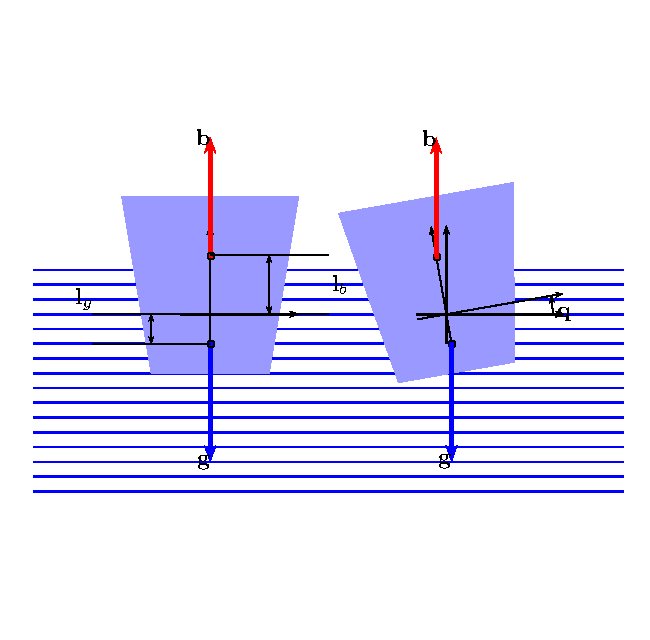
\includegraphics{ShipExample}
    \caption{The Floating Ship Example}
    \label{fig:ShipFloating}
  \end{center}
\end{figure}

The sway motion of the ship shown in Figure ~\ref{fig:ShipFloating} can be described by Equation~\ref{eq:shipflow}
\begin{equation}
\label{eq:shipflow}
J\ddot{q}+d\dot{q}=\tau(q)_{g}+\tau(q)_{b}+\tau_{u}
\end{equation}


where $q$ is the swaying angle.
$J$ is the inertia,  
$d$ is the damping coefficient,
and $\tau_{g}$,$\tau_{b}$,$\tau_{u}$ are the corresponding the torques of gravity, buoyancy and external control.

When a ship is on the sea, the motion is governed by the two forces, the buoyancy $b$ and gravity $g$.
When $\tau_{u}=0$,  the dynamics is becomes governed by its natural property.
Such a system is \emph{autonomous}.

To make it consistent with discussions in following chapters, Equation~\ref{eq:shipflow} is reformulated.
Defining the \emph{state} variable $\state=[q,\qd]$, then Equation~\ref{eq:shipflow} becomes
\[
\dot{\state}=F_{J,d}(\state)+Du
\]

where 
$F$ is a function of $\state$, the subscripts~$J$ and~$d$ are \emph{system parameters},
$D$ is a matrix, which describes how the control effort is applied,
and $u$ is \emph{control input}, for this example $u$ is $\tau_{u}$



\subsubsection*{Equilibrium Postures}
A ship will only rest when $\tau_{g}+\tau_{b}+\tau_{u}=0$, which are called \emph{Equilibrium} Postures.
The only two possible ones are show in Figure ~\ref{fig:ShipEqulibriumStable} and Figure~\ref{fig:ShipEqulibriumUnstable}.
\begin{figure}[!htbp]
  \begin{center}
     \includegraphics{leftPos}
    \caption{The Stable Equilibrium Posture}
    \label{fig:ShipEqulibriumStable}
  \end{center}
\end{figure}

\begin{figure}[!htbp]
  \begin{center}
     \includegraphics{rightPos}
    \caption{The Unstable Equilibrium Posture}
    \label{fig:ShipEqulibriumUnstable}
  \end{center}
\end{figure}



The two postures are different, illustrated with the \emph{phase plot}.
On the phase plot, the horizontal axis represents  $q$; and the vertical axis represents velocity $\qd$. 
The motion of the ship is shown as a curve on the phase plot, which is called \emph{flow}.

The posture in Figure ~\ref{fig:ShipEqulibriumStable} is \emph{attractive} or \emph{stable},
for if a small perturbation moves the ship away from the left posture, it will return to the equilibrium posture automatically as shown in Figure~\ref{fig:StablePosture}.
\begin{figure}[!htbp]
  \begin{center}
      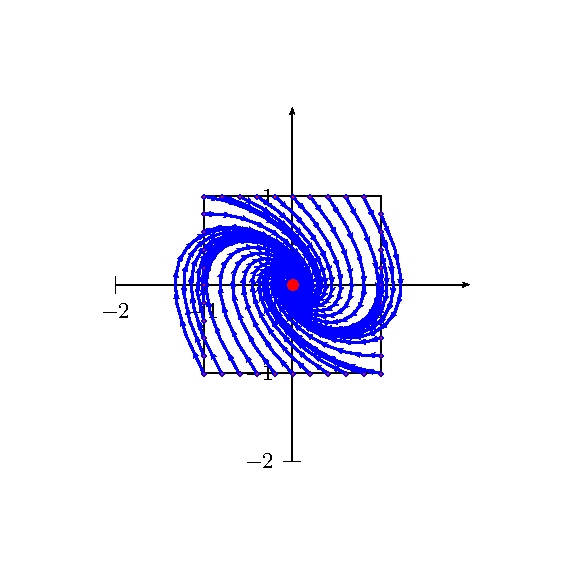
\includegraphics{stablePosition}
    \caption{Phase Plot of the Stable Posture}
    \label{fig:StablePosture}
  \end{center}
\end{figure}


Whereas the  posture in Figure~\ref{fig:ShipEqulibriumUnstable} is \emph{repelling} or \emph{unstable}, if being moved away from the equilibrium posture, the ship will move away further, as shown in Figure~\ref{fig:unStablePosture}.

\begin{figure}[!htbp]
  \begin{center}
      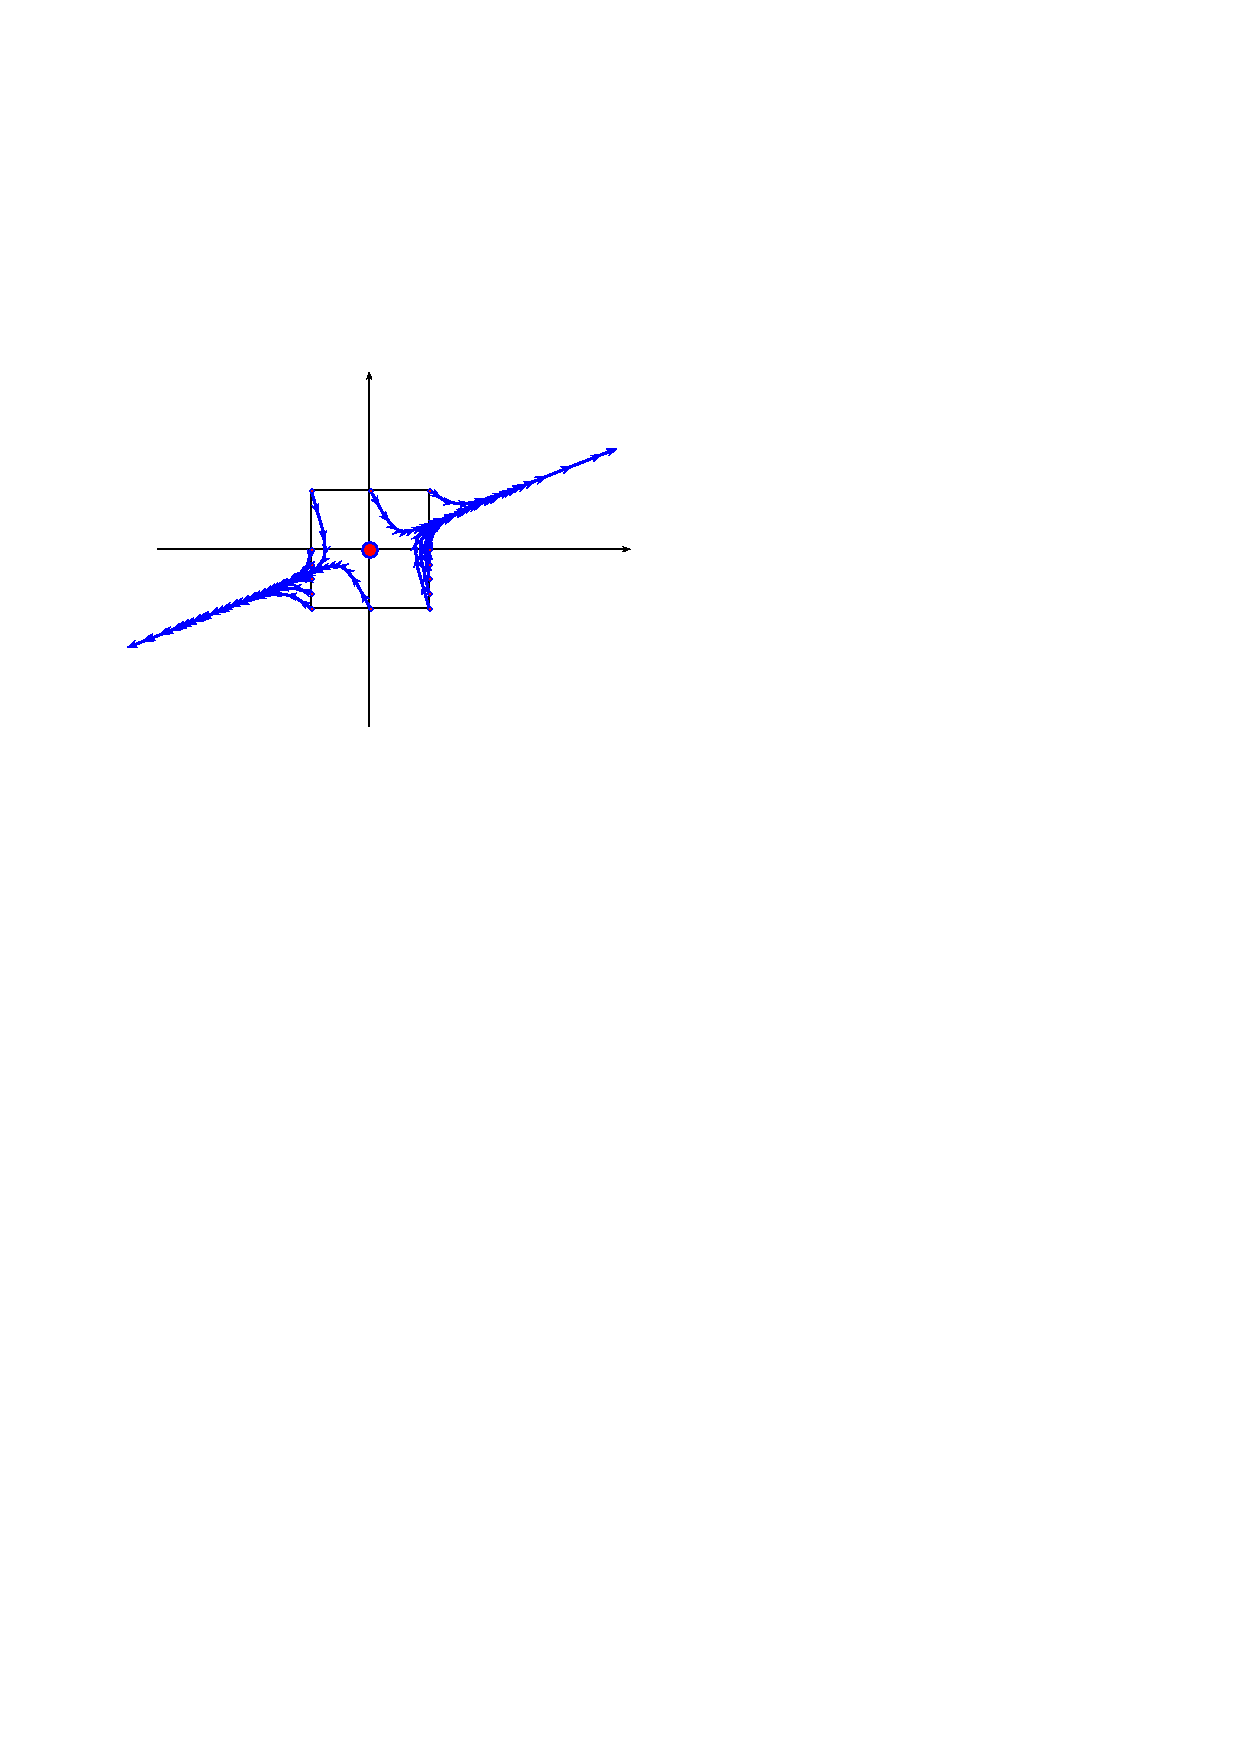
\includegraphics{unstablePosition}
    \caption{Phase Plot of the Unstable Posture}
    \label{fig:unStablePosture}
  \end{center}
\end{figure}


\subsubsection*{Trivial Task}
All the flows form the \emph{phase portrait} of the dynamic system. 
The discovery is that all the flows start from the repelling posture and ends at the attractive posture.
Several example curves are show in Figure ~\ref{fig:globalflow}.
This means no matter what the current posture is, the ship will return to the normal stable posture automatically.

This is an intrinsic property of the natural dynamics, and thanks to this, balancing is a trivial task which requires no control effort. 
This property is determined by the qualitative structure design criteria, makeing the centre of buoyancy  above the centre of gravity.

\begin{figure}[!htbp]
  \begin{center}
   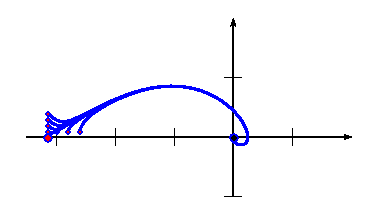
\includegraphics[width=0.7\textwidth]{ShipGlobalFlow}
   \caption{Global Properties of the Flows: All the curves start from the repelling posture(Red) and end at the attractive one(Blue)}
   \label{fig:globalflow}
  \end{center}
\end{figure}

 



\subsubsection*{Generalization of the Ship Example} 
This conclusion is independent of the shape, size, weight or material of the ship. 
In general cases, the same wave perturbation will result in different sway motions for different ships.
Howerver, as long as the qualitative structure design criteria is maintained, balancing remains ``easy''.
On phase portraits,  all the ships share following properties. 
\begin{itemize}
\item one repelling point 
\item one attractive point 
\item all flows start from repelling point and end at the  attractive point. 
\end{itemize}

In mathematical terms, all the phase portraits share the same topology structure of Figure~\ref{fig:topologyStructure}.

This phenomenon illustrates the principle idea of motion adaptation in \moit.
When the variations among individuals or situations result in motion variation, the qualitative dynamics or topological structure of the dynamic system remains invariant.

\begin{figure}[!htbp]
  \begin{center}
   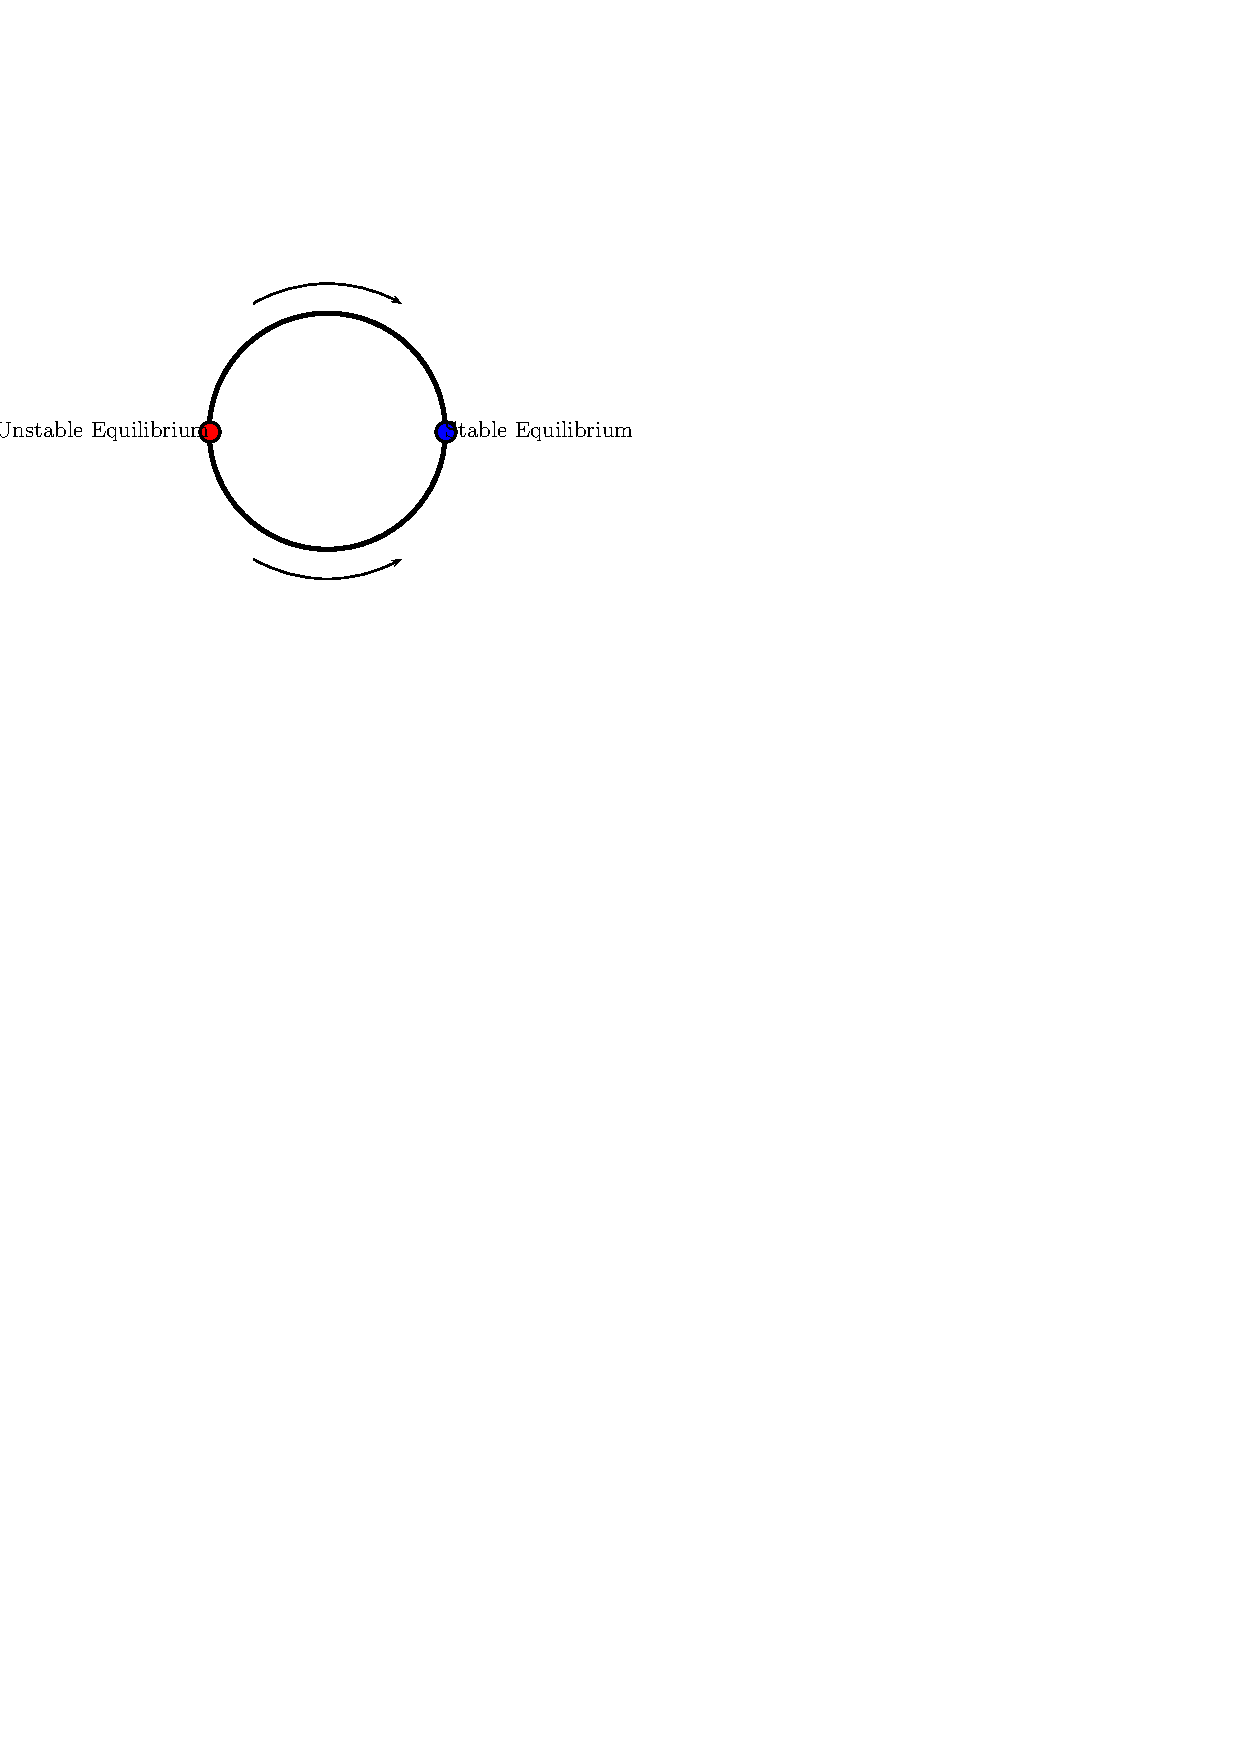
\includegraphics{topologyStructure}
   \caption{the topology  the phase portraits of ship dynamic}
   \label{fig:topologyStructure}
  \end{center}
\end{figure}




\subsection{The Mass Spring System:  Symmetry Transformation}
Despite the complexity of body structure, biological motor control is fast and accurate.
Such quantitative properties pose another puzzle in motor control research, as solving the complex dynamics directly would require prohibitive long computational time and excessive mental resources.

\moit proposes a new method to achieve the  speed and accuracy of motor control.
An efficient control strategy is based on the idea of transformation.
Without solving the dynamics, new motions are achieved through transforming template motions.
To keep the motion natural looking, control system chooses the transformation directions that are energy efficient, or in another term, allowed by the natural dynamics.


Such ideas can be illustrated by the following mass spring example, shown in Figure~\ref{fig:massspring}.
The mass spring system is selected for it captures some important properties of biological dynamics.
The compliant actuators of muscles work like springs, and rigid bones are modelled as mass.


\begin{figure}[!htbp]
  \begin{center}
    \includegraphics[width=0.7\textwidth]{MassSpring}
    \caption{the mass spring system}
    \label{fig:massspring}
  \end{center}
\end{figure}

\subsubsection*{Dynamics}
The canonical equation of mass spring system is
\begin{equation}
\label{eq:mass-spring}
\ddot{q}+q=0.
\end{equation}
where $q$ is the offset distance.

By defining the \emph{state variable}, $\state=[q,\qd]$, Equation~\ref{eq:mass-spring} can also be reformulated in the form as
\[
\dot{\state}=F(\state)
\]

 Figure~\ref{fig:massSpringPhasePlot} shows two flows passing through different states $x$ and $x'$ on the phase plot.


\begin{figure}[!htbp]
  \begin{center}
     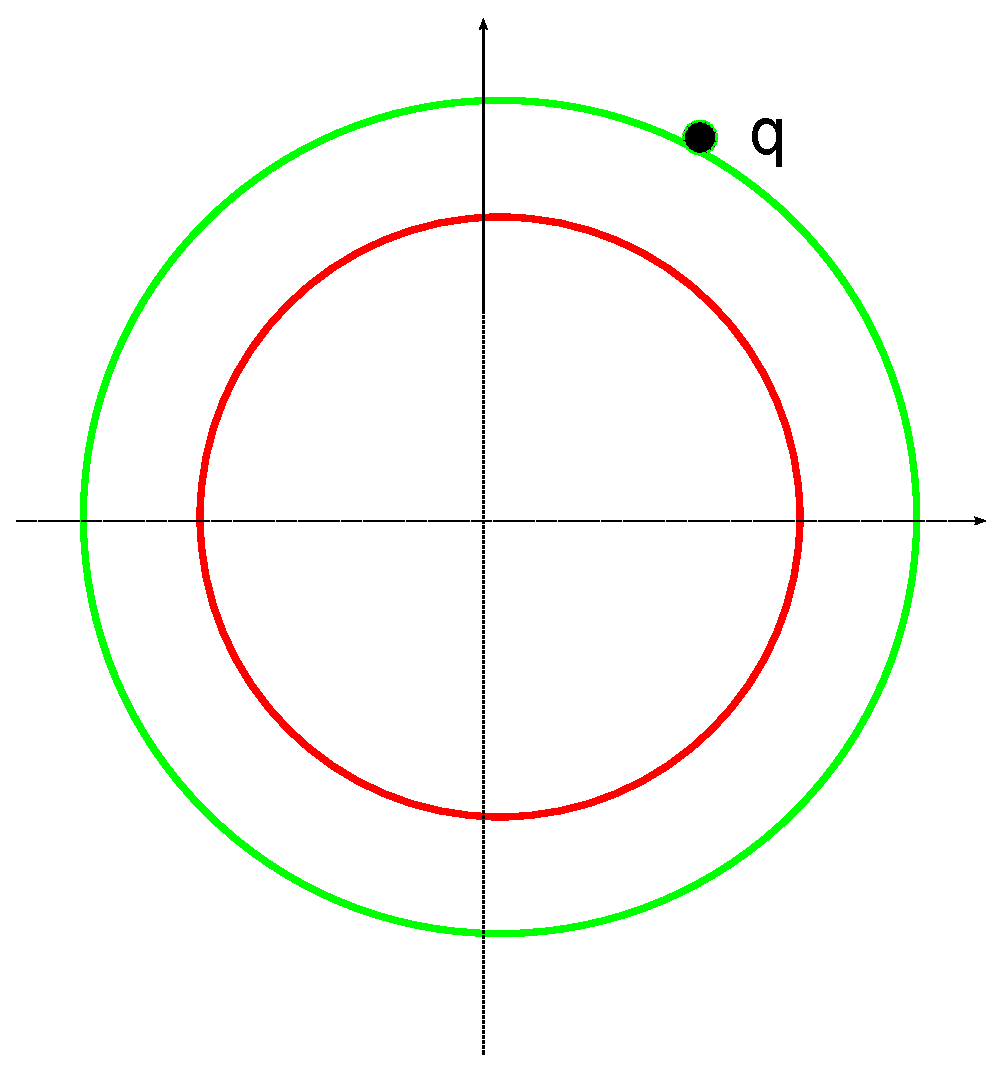
\includegraphics[width=0.5\textwidth]{MassSpringPhasePlot}
    \caption{Mass Spring Phase Plot:two motion curves are shown.The red one and the green pass through different states ($\state$ and $\state'$}
    \label{fig:massSpringPhasePlot}  
  \end{center}
\end{figure}

\subsubsection*{Symmetry and Transformation}
%It is highly unlikely animals can solve Equation~\ref{eq:mass-spring}.

The mass spring system has some ``symmetrical properties''.
Different flows share the same circle ``Shape''.
Without sovling the Equation~\ref{eq:mass-spring}, neew flows(solid ones) can be obtained by scaling the original(red) flow.

From a mechanical viewpoint, this is because the flows of mass spring system are energy preserving.
We can define the energy function
\[
E=\frac{1}{2}(m\qd^2+kq^2)
\]
where $k$ is the stiffness, $m$ is the mass.
When $m=1,k=1$, since $E$ is a constant, we can take $E=c$,
and obtain $q^2+\qd^2=2c$, which is the implicit function of a circle.

Therefore, given the template flows that pass through  $\state$, for the state $\state'$, by checking the energy, the scale transformation from red to green can be worked out.
In this manner, we botained the future motion after $\state'$, without sovling the dynamics.


\subsubsection*{Dynamic Perception and Local Motor Invariant}

The idea ``transformation and symmetry'' may shed light on dynamic perception. 
It is highly unlikely animals can solve Equation~\ref{eq:mass-spring} to understand mass spring system.
As an alternative, the dynamics can be encoded in a different manner: a motion template and the symmetry property. 
If so, observed motions can be validated by being checked against motion templates in our memory.

To make it better, it is even unnecessary to working out the transformation, it is enough just to check some property invariant under transformation.
For the mass spring system example, we can check the “shape” of the flow, or from a mechanical perspective, check the energy preserving property.

 
The invariant properties like energy preserving or shape can be quantitative measured, they are invariant only when system flows move in a specific direction, thus are called  \emph{Local Motor Invariant}. 


\section{Contribution}

Compared with current \cms methods, the new approach has several advantages:
\begin{enumerate}
\HiItem {More Types of Adaptation}
Most dynamic methods only focus on generating responsive motion to dynamic perturbation.
Adaptations across different characters are solved with a different method and treated as a independent research topic(motion re-targeting).
\moit unifies different  adaptations in one theory.
The mathematical idea of topology conjugacy  incorporates both motion re-targeting and  perturbation responses  in an unified framework.
Thus \moit can generate more types of adaptation.
\HiItem {Better Usability}.
For many \cms methods, each \dof ~is controlled independently.
When modifying motions, animator has to modify each \dof, which is tedious work.

In \moit, adaptation is achieved by applying transformation.
Each transformation can be parameterized by one parameter. 
By specify only one parameter for the transformation, control inputs of all {\dof}s are modified automatically, which is more easy to use.

\HiItem {No Reference Motion Needed}
\moit relies on the dynamics of body and environment.
Motion Capture Data is not needed as reference input.
In situations, this method can generate new motion that can not be captured.


\HiItem {Computationally Efficient} 
This motion synthesis approach requires little computation time and memory, it suits real-time applications.
\HiItem {Dynamic Motion Transition}
Dynamic motion transition is developed upon solid theory foundation.

\end{enumerate}

Because of its biological foundation,
algorithms and simulation results of \moit  might shed light into biology research.
Some conclusion and control techniques can be treated as candidate theory that needs further verification.

\begin{enumerate}
\item 
Motion Primitive is an old idea in biological research, but there is no agreement on the definition and underlying reason.
Biological research has tried to identify motion primitive by exploring the neural anatomy, EMG signal or muscle activation pattern.

\moit  explains the motion primitive from dynamic viewpoint.
This theory is more complete.
Besides identification, it also answers why certain motions are primitives and others are not,
how many motion primitives we have,  and where they come from.

\item One supporting theory of motion primitive is the muscle synergy:
Generating motion by actuating muscles, muscles are not controlled independently but worked in group. 
Many research in synergy by empirical methods. 

In \moit, when control is applied to ensure transformation, actuators are controlled in an ``synergy manner''.
\moit provides a candidate  ``synergy'' method for muscle control.

\item For the neural structure \emph{Central Pattern Generator}(\cpg) , their roles in motor control are well agreed.
While detail strategy for adjust \cpg parameters according to motor purpose is still lacking.
The \moit provides an theory for modifying the \cpg parameters with mathematical rigidity.


\item  Motion and dynamic perception mechanism of neural system is still unclear.
The motor invariant theory proposes a computationally efficient mathematical machinery.
\end{enumerate}







\section{Organization of the Thesis}

This thesis is organized as follows.
 
In Chapter~\ref{chap:background}, previous research on motion synthesis and biological motor control are discussed, which are the motivation and justification of \moit.
 
In Chapter~\ref{chap:gi}, \emph{Qualitative Dynamicss} is introduced to explain motion primitives. 
Biological based  methods for maintaining the global motor invariant are developed.

Chapter~\ref{chap:li} focuses on the idea of Local Motor Invariant and Symmetry.
Lie Group theory is  introduced  to analyse the symmetry properties in motion dynamics.
Symmetry Controllers are developed for adaptation motions.
 


Chapter~\ref{chap:msf} discusses the combination problems.
For each motion primitive,  strategies are developed to preserve global and local motor invariant simultaneously.
Motion primitive transition is discussed and methods for combining motion elements into more complex motion is discussed.
As an animation system, the software architecture and work flow are discussed at the end.

Chapter~\ref{chap:gi},~\ref{chap:li},~\ref{chap:msf} lay the theoretical foundation of \moit.
Following chapters focus on application in \cms.



Chapter~\ref{chap:walk} focuses the tweaking of one primitive.
Bipedal walking is chosen, which is one of the most challenging problem for current \cms research.
Motor Invariant Theory introduces a method to boost the stability and generate adaptive gaits.


In Chapter~\ref{chap:stance}, combinations of motion primitives are discussed.
A new balancing motion primitive is developed. 
Transitional motions are generated for stance to walk and walk to stance transitions.

In Chapter~\ref{chap:highdor}, extensions of motor invariant theory to more complex characters are discussed.
Three strategies are developed to simplify the problem for different situations.

This thesis ended with Chapter~\ref{chap:con}. 
After discussion of new finding of this research, some new questions and ideas for graphics and neural science are proposed for further research .





%%% ----------------------------------------------------------------------


%%% Local Variables: 
%%% mode: latex
%%% TeX-master: "../thesis"
%%% End: 


\chapter{BACKGROUND}
\label{chap:background}

\nomenclature[z3]{\pd}{Proportional Derivative}
\nomenclature[z4]{\lc}{Limit Cycle}
\nomenclature[z5]{\cpg}{Central Pattern Generator}
\nomenclature[z6]{\eph}{Equilibrium Point Hypothesis}
\nomenclature[z7]{\umh}{Uncontrolled Manifold Hypothesis}
Underneath different \cms methods, are different ideas of motor control.
Current \cms research follows the control idea for artificial system.
There is a clear speration of planning and execution in traditional controller design.
In the \cms research, body are treated as mechanical apparatus, which execute the motion planned by the neural system.

Motor Invariant Theory is based on the intergrative theory of motor control\citep{dickinson2000animals}.
In the integrative view, there is no a clear seperation between planning and execution,  motor control can only be understood as a whole.

In this chapter, limitation of current \cms research are discussed first for they are the motivation of this research.
New theory is developed because such limitations can not be overcome within the current framework.

Later some biological research are discussed later, for they are the foundation upon which motor invariant theory is built.
Biology research provide the justification for the new \cms method.



\section{A survey of \cms}

Many methods are developed in \cms research.
It is impossible to include all the research work and discuss the difficulties one by one.

In the short discussion, different \cms methods are categoried by the control model: memory or computational.
Memory model inspired the data-driven techniques.
Procedure methods folloiwng the computational principle.
Pros and cons are discussed category by category.

\subsection{Data Driven}
Data-driven methods are based on ready motion data which are generated by Key-frame or Motion Capture(Mocap). 
In practice, motion data are segmented into short time clips. 
An animation is generated by selecting motion clips and connecting them together\citep{Parent2002,kovar2003flexible}.

Like other example based methods, data driven methods can generate good results if similar motion clips can be found, but it is difficult to generate  motion adaptation, whether for a different character or a different scenario. 
This is usually referred to `` the motion re-targeting'' problem.

Besides the limitation in new motion generation, management of large motion data is another problem in practice. 
The Annotation Database \citep{Arikan2003} and the Motion Graph \citep{kovar2008motion}are proposed for organizing motion data. 
Currently, catalogue and search of motion data are not trival and remain open\citep{keogh2004indexing,muller2005efficient}.

\subsection{Procedure Method}
For physics based \cms, different approaches have been proposed.
\begin{itemize}
\HiItem{Propotional Derivative (\pd) Controller}

\pd controller works in the reference tracking manner.
\begin{equation}
\label{eq:pdcontrol}
u=K(q -q_d)+d\qd
\end{equation}

Some early research applied classical \pd controller \citep{Raibert1991} for synthesizing.
Later research \citep{Hodgins1995} applied the same method for different tasks like running, bicycling, vaulting and balancing. 
For high dimentional characters, \pd controller tracking the predefine motion curves\citep{Yin2007}.

\pd control based method can run in real-time and generating adaptive response to small perturbation.
Large perturbation or deviation from the reference trajectory are difficult to achieve with \pd controller.








\HiItem{Limit Cycle}
Most \pd based controllers use motion capture data as references.
\citet{Laszlo1996} introduced limit cycle (\lc) as tracking reference lower energy locomotion animation. 
Limit Cycle arises from natural dynamic property.

Limit Cycle methods share many characteristics with \pd.
In current researches\citep{Coros2009,Laszlo1996} track fixed limit cycle, and can generated very limited motion adaptation.



 


\HiItem{Optimization}
Because of the redundant \dof s, motion plannig is nondeterministic.
For the problem, optimization has been introduced.
The idea is among all the possible motions, the ``best'' one is choosn.

Many metric has been proposed for optimization, 
For dynamic methods, a reasonable method is try to find the motion cost least energy~$E$. 
\begin{equation}
 \textbf{E}=\int_{t_0}^{t_1}f_{a}(t)^2dt
\end{equation}
where $F_{a}$ is the active force generated by actuators like motors or muscles. 
This is introduced to \cms research as the influential Spacetime Constraints\citep{Witkin1988}. 
It is based on the hypothesis that the natural looking trajectory costs minimum energy. 
It is related to the idea of Darwin's Theory of Evolution and the principle of Natural Selection. 
In many cases, these methods produced very believable motions. 
\citet{Jain2009} provides an example of locomotion.  
\citet{BalanceControl} find a method for balance maintaining movement. 
\citet{Liu2009} proposed a method for object manipulating animation. 
\end{itemize}
\subsubsection*{Drawbacks of Optimization}
Optimization is the current mainstream method for physics based animation.
It generated the best motion results in current research.
But this method has several drawbacks.

\begin{itemize}
\HiItem{Numerical Stability and Modelling Difficulties: }
Optimization methods promise the energy efficiency of the resulting motion, but no garantee about convergence speed and stability.
Optimal solution is difficult to find numerically, and are sensitive to the accuracy of the model and the proximity of the initial guess.
\citet{Liu2005} points out those space–time constraint methods only suit high energy motions, like jumping and running.
For low energy tasks (such as walking) the results do not look natural.

\HiItem{Computational Complexity: }
Optimization with space–time constraints is a variational problem by nature. 
For a complex characters, it might takes  prohibitively long time, limiting the application domain of problems to those which are computationally feasible. 
In addition, little is known about how to reuse a computation result for motion adaptation.

\end{itemize}


\subsection{Biological Constraints}
The problems of \cms has also been spotted earlier by bilogical motor control.
The theory from tradition artificial systems such as \pd or optimization, are highly unlikely the priniciples for biological motor control, for they  violates the biological constraints.
Although the mechanism behind information processing remains obscure, some characteristics of biological information processing are well agreed, which make  \cms methods above questionable\citep{Glynn2003}. 
  
\begin{itemize}
\HiItem{Sensing and Control Limitations:}
Motor control is not only a mechanical problem, but a complex process involves chemical, electrical changes.
Many crucial mechanical parameters and variables such as mass, inertia, force, are inaccessible to the neural system and can only be approximated. 
For important control variables (such as torque), the neural system controls indirectly through a complex process.
Also body and environmental measurements are noisy and time varying, making methods that are sensitive to errors unsuitable for biological motor control.

\HiItem{Neural Computation: }
The neural system is powerful, but is inferior in speed and accuracy when compared with a digital computer. 
It can only generate signals at hundreds of Hz, signal transmission speeds are slow, and there is a long delay between firing a neural signal and generating force in the muscles.
it may cost about half a second from seeing an object to force generation in arm, . 
This makes it impossible for the neural system to carry out the complex computation necessary for real–time optimization.


Following the idea of optimization control, the dynamics of fluid environment and deformable body are more difficult to optimize. 
But most primitive life forms live in the sea and have limited intelligence. 
\HiItem{Memory Capacity:}
Some people argue that motion control is not based on computaion, but based on memeory.
This idea may helps to drop the question of computation speed, but it faces the memory capacity problem. 
Motion varies greatly, if we store the motion in our brain, the problems is the memory capacity.
\end{itemize}

\section{Motion Primitives}
Many animals include human exhibit complex motion behaviours at very young age.
Many complex motion behaviour like breathing, heat beating and child bearing are inborn ability without the need for learning.
These evidence suggests that motor ability may organized in blocks\citep{bizzi1995modular,bizzi2002book}.
Strong evidences come the experiment of stimulating of a single spinal motor afferent triggers a complete sweeping motion\citep{bizzi1995modular}.
The number of motion primitives is limited.
Complex motions are combinations of motion primitives, just like we connect alphabets into sentences.
Such building blocks are called \emph{motion primitives}.
Motion primitives are also give insight into the motion preception.
\citet{gallese1996action} have found action and perception trigger similar reactions in a group of neurons.





\subsection{Dynamic Motion Primitives}
It is impossible in reproduce the whole body and neural system in computer to produce character motions.
For dynamic \cms, the key question is how motion primitives simplify the dynamics of motor control.

An alternative idea that animals don’t move the way they want, but rather the way they can. 
Motion style is not changed much by the neural system evolution, after all whale swim more like fish than other mammals.
The motion style is close related to the body structucture and environment.
These finding lead us shift our focus away from the neural system and understand motor control through an integrative view which incoporate neural system, body strucuture and environment\citep{dickinson2000animals}.
The body and the environment play the most important role in motor control, as they form the basic pattern of motion \citep{nishikawa2007neuromechanics}.


Follows the questions of motion primitive models.
Motion primitive should not be a trajecotry tracking system.
For even under the same conditions, the motions still vary. 
Some \dof s are not controlled and freely influenced by the environment. 
\emph{Uncontrolled Manifold Hypothesis(UMH)}\citep{latash2008neurophysiological} propose in motor control, trajectory is not concern, only the final results is.


\emph{Equilibrium Point Hypothesis(EPH)}\citep{Feldman1986} is a specification of UMH for . 
This idea comes from properties of differential equations. 
For a dynamic system
\[
\dot{\state}=F(\state)
\]
the equilibrium points $\state_{e}$ satisfy the condition $F(\state_{e})=0$.
EPH suggests that what the neural systems controls is not trajectory, but the equilibrium points.



\emph{Impedance Control} \citep{hogan1985ica} refines the idea of EPH by providing an explanation for effects of the extra DOFs. 
At an equilibrium point $\state_{e}$,
\[
F(\state_{e})=0 
\]
Impedance Control proposed that the extra DOFs provide a way to control the stability and admittance of the equilibrium point $_{e}$. 
The mathematical presentation is
\begin{equation}
F(\state_{e}+E_r)=KE_r
\end{equation}
where $E_r$ is the offset error vector, $K$ is stiffness matrix or impedance,will determines the stability.
Neural system will tune the direction of $K$ according to the motion purpose, such as avoiding obstacles and risks. 
Experiment \citep{Franklin2007} shows that the matrix $K$ has anisotropic properties.







\subsection{Neural Control Model}
Human motor control involves little mental work.
The current idea of biology research is that motor control is a low level intelligent activity and can be controlled  without brain input. 
Two models are developed for ``tweaking'' motion primitives.
\begin{itemize}
\item
In vertebrate animals,  Central Pattern Generator (\cpg) serves many functions in locomotion, respiration and swalling and other rhythm behaviour.
\citet{Cohen1988a} argues that locomotion is the result of the interaction between neural and mechanical oscillators via a process called \textbf{entrainment}.
Neural systems modify the motion by adjust frequency and amplitude of neural rhythmic signal.



\item
Some research find motion will change in a uniform manner\citep{Viviani1992},\citep{flash2007affine} propose modeling motion adaptation through \emph{affine transformation}.
Both works implies close relationship between motor control and the vision system.
\end{itemize}









\subsection{ Evidences from Bionomic Robotic Research}
Biological research idea greatly inspired the engineering experiment.
Some researches begin to focus on utilizing the natural dynamic follow the biological motor control principle.
And some significant result has been reported
\begin{itemize}
\HiItem{Limit Cycle in Walking}
A very important discovery is the bipedal walking can happen without any control\citep{McGeer1990}.  
And based on this idea, new mechanical system is designed that can walk on plane with simple control stragety\citep{Collins2005}.

\HiItem{\cpg and entrainment}
The \cpg based entrainment is applied for robotic research\citep{Williamson1999a}, the finding results show the CPG will boost the system stability and can maintain motion in unpredictable situation.

\HiItem{Control Symmetry}
Symmetry is also well exploit in Mechanical research as conservative laws.
The idea of Symmetry is also used in control robotics\citep{spong2005controlled}.
\end{itemize}

\section{Placement and Contrasts}
This biological research ideas are the foundation upon which the motor invariant theory is built.
The mathematical concept of topological conjugacy is introduced to generalize and unify different ideas.

Motion Primitives comes from the \emph{structual stable} component in natural dynamics.
\eph and Impedance Control are generalized as control of attractor and attractivity.

\cpg and Transformation are different in principle, there is no research attempts to unify the two ideas in one motor control framework.
Motor Invariant Theory include both methods for a good biological reason: \cpg comes from the research of functions of spinal cord, which models the low level control; while the transformation idea comes from search of the cortex, which is a model for high level control.
 
Within Motor Invariant Theory,  \cpg and transformation works as complementation.
\cpg boost the stability of motion primitives though entrainment, it works as a low level qualitative control mechanism.
Transformation adapt motion for task specific purpose, it is more precise and serve as quantative control.

Motor Invariant Theory also extend current biological research by include motion primitives transition.


 

 




\chapter{GLOBAL MOTOR INVARIANT}
\label{chap:gi}
\section{Introduction}

\nomenclature{$q$}{Generalized Coordinates}
\nomenclature{$Q$}{Configureation Space or Configuration Manifold}
\nomenclature{$\qd$}{Gneralized Velocity}
\nomenclature{$TQ$}{Tangenet Bundle of $Q$}
\nomenclature{$u$}{Control Input}
\nomenclature{$\state$}{State Variable}
\nomenclature{$M$}{State Space Manifold}
\nomenclature{$TM$}{Tangent Boundle Manifold}
\nomenclature{$A$}{Attractor}
\nomenclature{$B(A)$}{Basin of Attration of $A$}
\nomenclature{$S$}{Neural Oscilator}
\nomenclature{$\uin$}{Input Signal to the Neural Oscilator}
\nomenclature{$\uout$}{Output of the Neural Oscilator}
\nomenclature{$\hin$}{Input Coefficient of the Neural Oscilator}
\nomenclature{$\hout$}{Output Coefficent of the Neural Oscilator}
\nomenclature{$\simeq$}{Topology Conjungacy}


%\nomenclature[zcif]{$CIF$}{Cauchy's Integral Formula}                                % first letter Z is for Acronyms 
%\nomenclature[aF]{$F$}{complex function}                                                   % first letter A is for Roman symbols
%\nomenclature[gp]{$\pi$}{ $\simeq 3.14\ldots$}                                             % first letter G is for Greek Symbols
%\nomenclature[gi]{$\iota$}{unit imaginary number $\sqrt{-1}$}                      % first letter G is for Greek Symbols
%\nomenclature[gg]{$\gamma$}{a simply closed curve on a complex plane}  % first letter G is for Greek Symbols
%\nomenclature[xi]{$\oint_\gamma$}{integration around a curve $\gamma$} % first letter X is for Other Symbols
%\nomenclature[rj]{$j$}{superscript index}                                                       % first letter R is for superscripts
%\nomenclature[s0]{$0$}{subscript index}                                                        % first letter S is for subscripts



\ifpdf
    \graphicspath{{GlobalInvariant/GlobalInvariantFigs/PNG/}{GlobalInvariant/GlobalInvariantFigs/PDF/}{GlobalInvariant/GlobalInvariantFigs/}}
\else
    \graphicspath{{GlobalInvariant/GlobalInvariantFigs/EPS/}{GlobalInvariant/GlobalInvariantFigs/}}
\fi

Motion varies greatly, different people walk with different gait. 
A question is why the different motions of different people are all called walk.
Our answer is walk is not determined by the details how it is carried out.
Walk capture the qualitative properties, and we agree on the walk becomes it is a property encoded in all our body, we all have the walking ability inborn, so that’s the reason why we can all identify it.


Our basic idea is motion primitives are ''easy'' to finish. 
In this chapter, we will try to give the “easiness” definition.
The biological ideas can be provide a clear mathematical meaning.


\section{Basic Concepts of Qualitative Dynamics}
This section develops the mathematical conceptualization of Global Motor Invariant.
Some mathematical background is needed in this discussion.
Throughout this paper, we take the geometrical viewport of mechanical system.
For analyzing qualitative properties, we introduce the ideas from differential topology.
This idea can be traced back to Poincare\citep{Poincar'e1899,Poincar'e1885} and recently developed by the Smale School\citep{Smale1970}.
It is impossible to put the a whole discipline in one chapter.
Please refer to other books and lectures such as \citep{abraham1978foundations}for introduction in details.


Dynamic motions are modelled as differential equations,
In the geometrical viewport, differential equation describes a differentiable manifold.
Qualitative Properties can be obtained by analyzing the topological structure of the differentiable manifold.
Global Motor Invariant is defined by the topology structure.



\subsection{Dynamic System and Differential Manifold}



The dynamic of a mechanical system is determined by its configuration  $q$ and generalized speed $\qd$. 
we represent the state of a system as a vector $\state=[q,\qd] \in M$,  $M$ is the state space, or state manifold.
The motion is a trajectory $t \mapsto q(t)$ in the configuration space parameterized by time~$t$.
For a dynamic system, $q(t)$ usually is derived from the state trajectory $\state(t)$, which is described by differential equaiton. 


For every point $x \in M$, 
$F$ and $u$ determines a derivative vector $\dot{x} in T_{x}M$ in the Tangent Space. 
All the vectors over the full space of $x$ form the \textbf{vector field} $\mathbf{V}$,describe by the differential equaiton~ \ref{eq:ode}
which described by the differential equation
\begin{equation}
\label{eq:ode}
\dot{\state}=F_a(\state,u),\state\in M
\end{equation}

where $u$ is the control effort. 
$a$ is the system parameters
$F$ is determined by the system's natural property.
If $u=0$,  no control effort is applied.
Such systems are \textbf{autonomous systems}. 

By solving the \textbf{intergral curve}to equation~\ref{eq:ode}, 
\textbf{flow} $\Phi(\state)$ of $\mathbf{V}$ is the \textbf{intergral curve} through $\state$. 
all the flows form the \textbf{phase portrait}, which illustrates all the possible motions of the dynamic system.
We usually visualize the differential manifold by \textbf{phase plot}.


An illustrative example repeatedly used in this report is the mass-spring system. 
After linear transformation,  
a linear mass spring system can be described in canonical form equation ~\ref{eq:mass-spring}
where $q$ is the position of the mass, $\qd$ is the speed, and $\ddot{q}$ is the acceleration of mass.
 
If we chose the state variable $\state=[q,\qd]$, the ODE model should be in the form of equation~\ref{eq:stateform}
\begin{equation}
\label{eq:stateform}
\dot{\state}=
\left[ 
\begin{array}{cc}
0 &1\\
-1 &0 
\end{array}
\right]\state
\end{equation}



\subsection{Global Motor Invariant}
Flows can only intersect at some special position called \textbf{equilibria}.
Basically there are three type of equilibrium.
At each \textbf{equilbria}, 
the local space can be divided into three subspace of sub manifold: centre sub manifold, stable manifold, and unstable sub manifold.
\begin{description} 
\item[centre sub manifold]
If a flow $\phi$ pass through a point $\state_{c}$ on centre sub manifold $W_{c}$,
flow$\phi$ will remain on the Centre Manifold 
\[
\phi_{c}(t) \in W_{c}, t \in R
\]
 An equilibria must be on center manifold. 
\item [stable sub manifold]
For the flow $\phi_{s}$ passes through a point $\state_{s}$ on stable sub manifold $W_{s}$, the flow will finally converge to a no wandering point on centre sub manifold.
\[
\phi_{s}(+\infty)=\theta_{c}
\]
\item[unstable sub manifold]
For the flow $\phi_u$ passes through a point $\state_u$ on unstable sub manifold $W_{u}$, the flow will be repelled from the no wandering points on centre manifold.
An alternative perspective is the inverse of the flow converge to no wandering point. 
\[
\phi_{u}(-\infty)=\theta_{c}
\] 

\end{description}

The size and dimension of each sub manifold varies.
For some cases, the $W_{s}$ ( $W_{u}$) may not exist, 
this can be seen as the dimension of $W_{s}$($W_{u}$) is $0$.
\textbf{Attractors} are the equilbria where the whole local space is stable, the dimension of unstable submanifold is zero $\mathbf{dim}(W_{u})=0$.
\textbf{Repellors} are the equilibrias where the whole local space is unstable,the dimension of stable submanifold is zero $\mathbf{dim}(W_{s})=0$.







In theory, only observe the attractor of the dynamic system can be observed, motion task should be only rely on the attractor.
Two types of attrator are of great interest in motor control:(1) fixed point, as show inf Figure~\ref{fig:StablePosture},(2)Limit Cycle,as shown in Figure ~\ref{fig:limit_circle}

\begin{figure}
\begin{center}
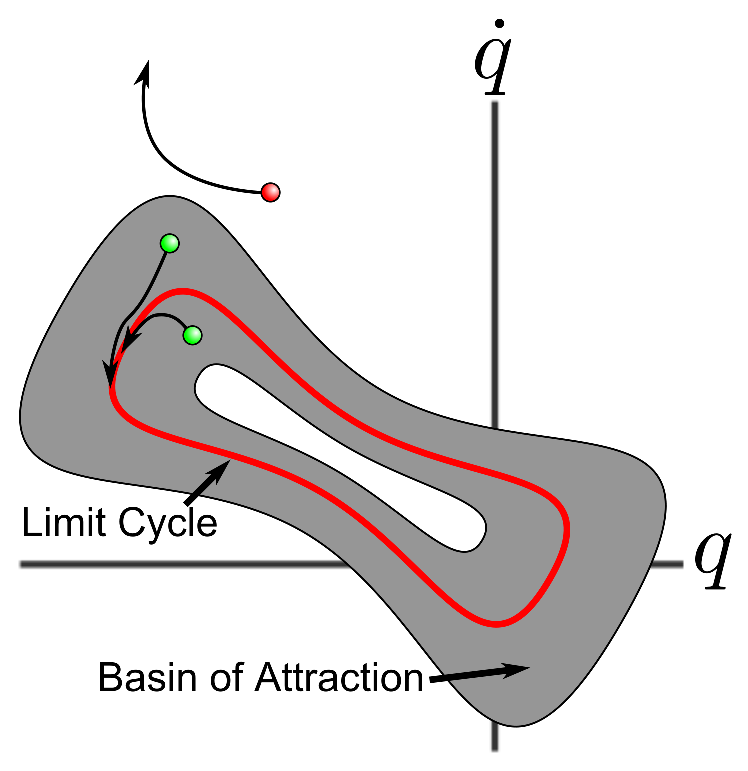
\includegraphics[height=0.4\textheight]{phase_plot}
\end{center}
\caption{Limit Cycle}
\label{fig:limit_circle}
\end{figure}




For nonlinear system, globally, the shape of stable and unstable sub manifold may be bending and connect with itself or each other.
The unstable manifold of one equilibrium may be the stable sub manifold of another.
The equilibra and its connectivity sub manifold form a topological structure.
Thus the phase plane will be divide into different regions,result in a cellular structure.
there is only one attractor, all the flow in this region will converge to the attractor ~$A$.
and the corresponding region is called basin of attraction ~$B(A)$.
as shown in figure~\ref{fig:manyboa}
\begin{figure}
\begin{center}
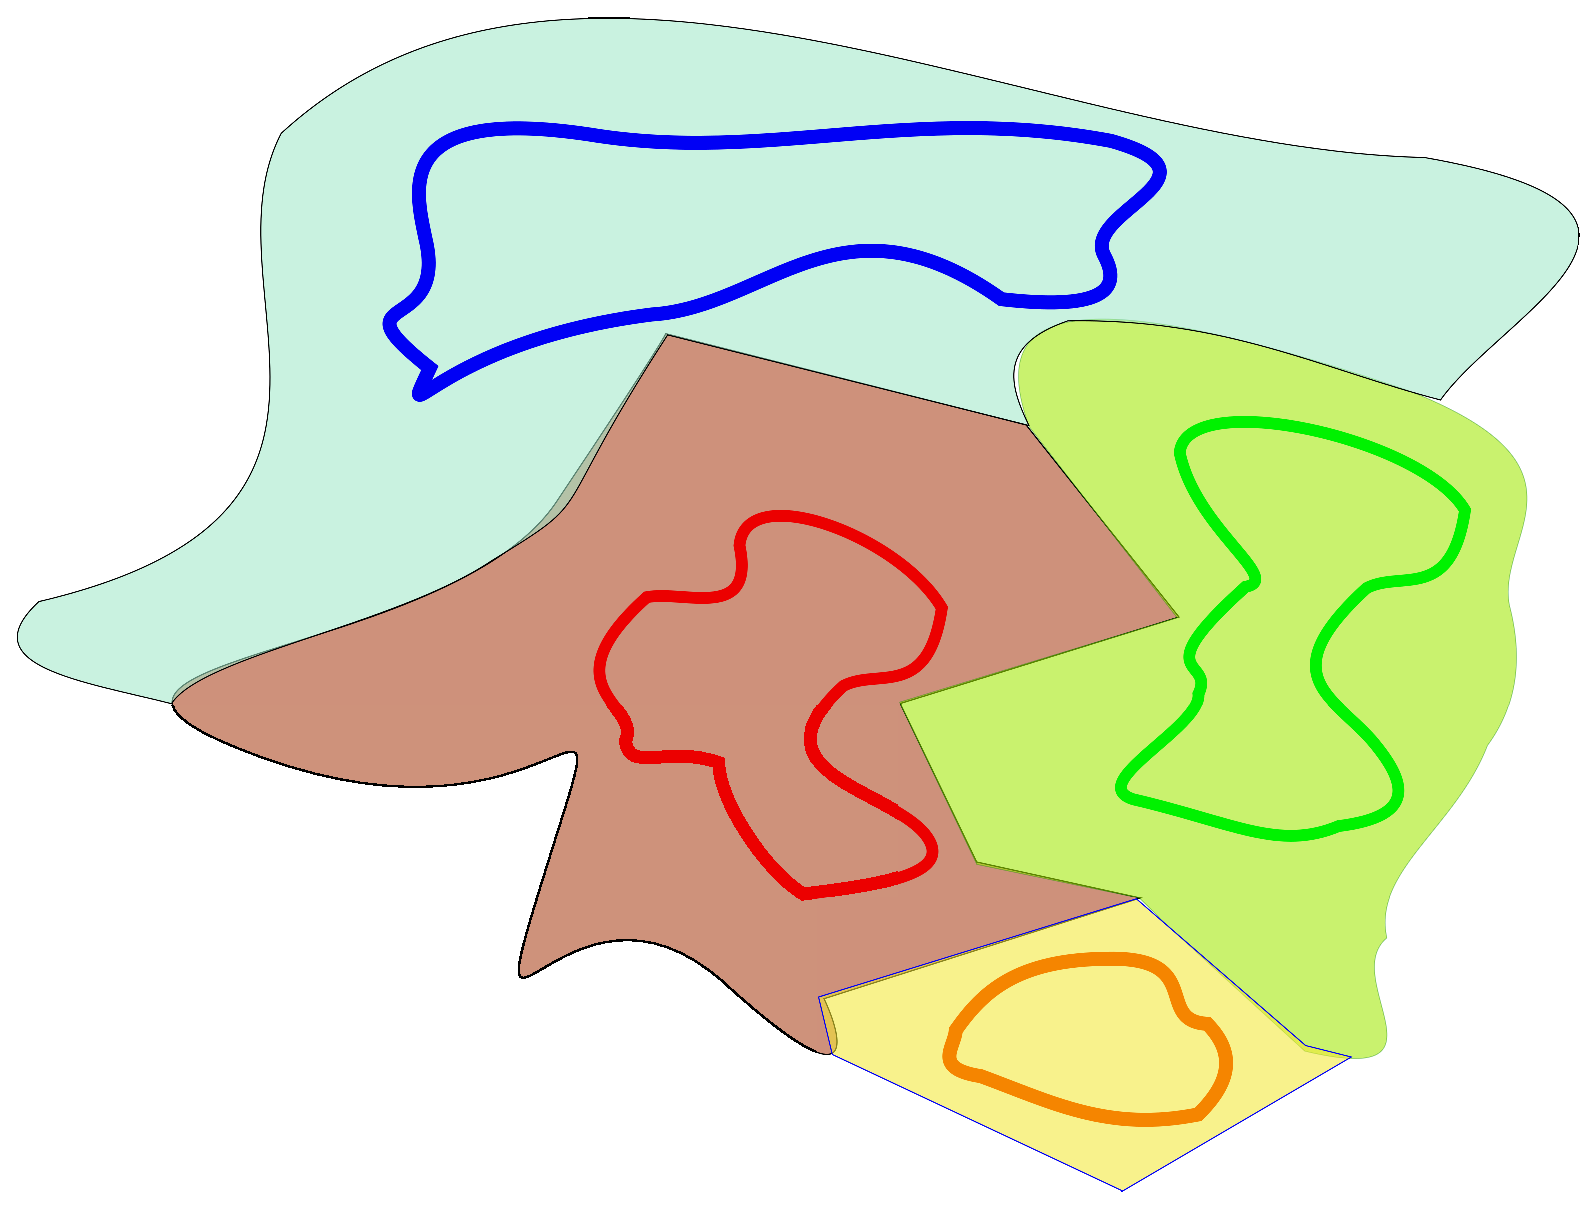
\includegraphics[height=0.4\textheight]{basinOfAttraction}
\end{center}
\caption{Celluar Structure of Phase Space}
\label{fig:manyboa}
\end{figure}


We can also give the biological ideas clear mathematical meaning.
The UMH, the uncontrolled manifold is the basin of attraction.
For EPH, the equilibrium point is the attractor.
For Impendence Control, impedance control is control the shape of basin of attraction.

\subsection{Analogous System And Topology Conjugacy}
many dynamic system are have different dynamic equation, but they share the same topology.
an example is the mass-spring system and the duffine system, described by equation ~\ref{eq:fuffin}
\begin{equation}
\label{eq:duffin}
\ddot{q}+q+q^{3}=0
\end{equation}
and the phase plot of the two system are show in figure~\ref{fig:msphaseplot},\ref{fig:duffin}

\begin{figure}
\begin{center}
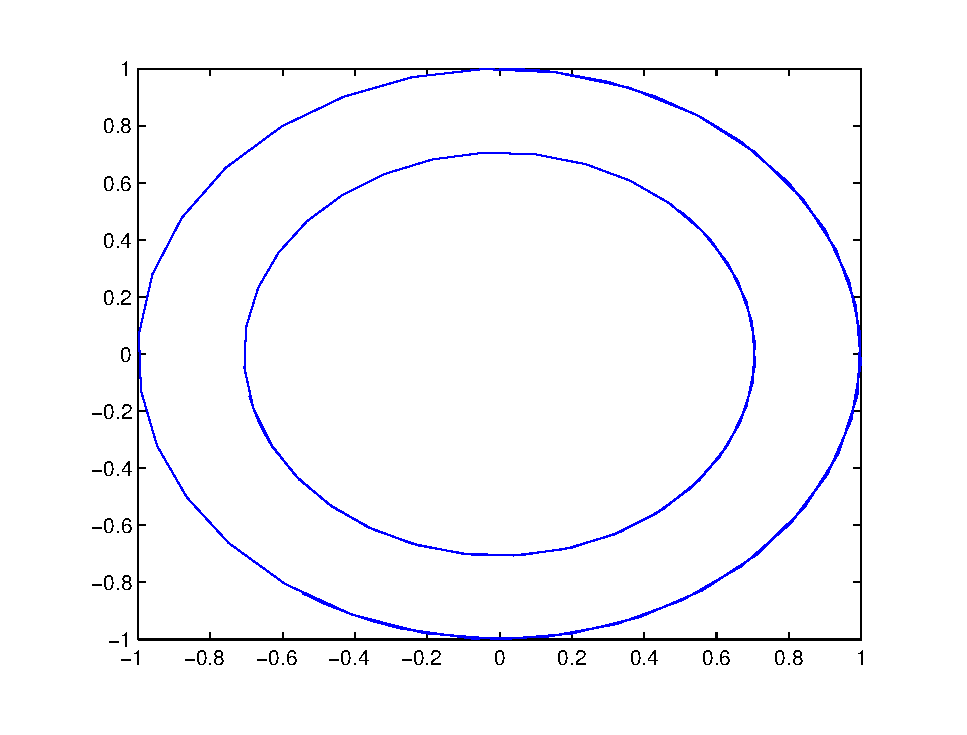
\includegraphics[height=0.4\textheight]{massspring}
\end{center}
\caption{Mass Spring System}
\label{fig:msphaseplot}
\end{figure}

\begin{figure}
\begin{center}
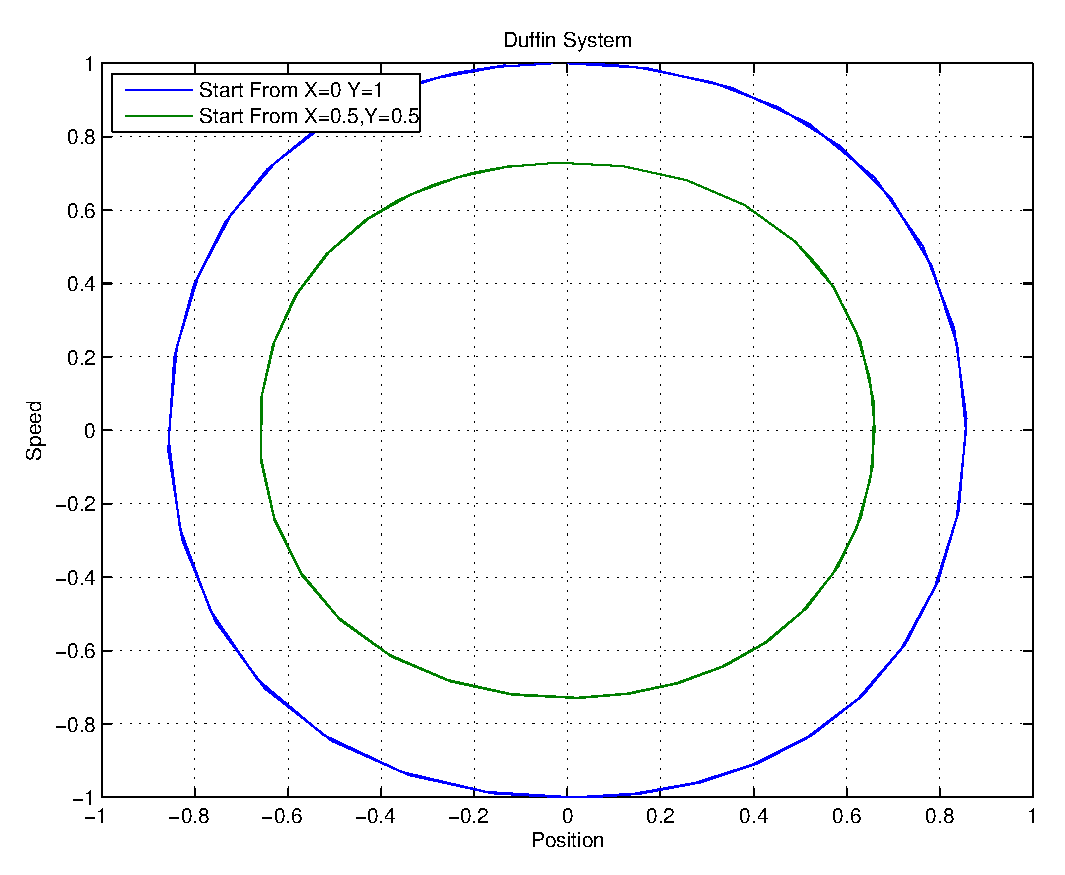
\includegraphics[height=0.4\textheight]{duffin}
\end{center}
\caption{Duffin Phase Plot}
\label{fig:duffin}
\end{figure}


one phase plot, the two system are similar, and we cand '' deform '' one into another.
in mathematical term, there is an equilalence relationship  for the two system. the \textbf{topological conjugacy}.

Let $X$ and $Y$ be topological spaces, and let $f\colon X\to X$ and $g\colon Y\to Y$
be continuous functions. We say that $f$ is
\emph{topologically semiconjugate} to $g$, if there exists a continuous
surjection $h\colon Y\to X$ such that $fh=hg$. If $h$ is a homeomorphism,
then we say that $f$ and $g$ are \emph{topologically conjugate}, and we call
$h$ a \emph{topological conjugation} between $f$ and $g$.



if two system are topological conjugate, they are analogous systems





\section{Global Motor Invariant and Motion Adaptation}
Global Motor Primitive is defined by the attractor type and its basin of attraction in the topology space.


Motion adaptation because of different reasons and in different situations.
Such two kinds of perturbation are treated separately and result in differentiation strategy or control.

\begin{itemize}
\HiItem{State perturbation}

The perturbation that move the state off the attractor is called State Perturbation, for only the state is changed, the dynamic system underline is not changed.


If the state is in the basin of attraction then, it will converge to the attractor. 
Start from different state position, it will result different flows, thus different motion.

Such kind of motion adaptation is called Responsive Motion Adaptation.
Because usually, for characters, perturbation comes from the push or pull, while the character and environment is not changed.

To make the character more responsive without result in motion failure,
Motion controller should try to enlarge the basin of attraction.






\HiItem{Structure Perturbation}

Another type of Perturbation will affect the dynamic system; such kind of perturbation is called Structure Perturbation. 
Such kind of perturbation happens commonly in our daily life, when a man put a heavy box on his shoulder, it will result a change in the dynamic system.

Structural Perturbation will change the phase portrait; some perturbation will make the system into an analogous system.
As a result, the even the current state is on the attractor, motion will change, this kind of motion adaptation is called system adaptation, and one important application is dynamic motion retargeting, when you change the character, the dynamic system changed.

Sometimes it will change the topology the underlying dynamic system, such effects are called bifurcation.
an example is the damping effects on the mass spring system.
as show in figure~\ref{fig:dampmass}

\begin{figure}
\begin{center}
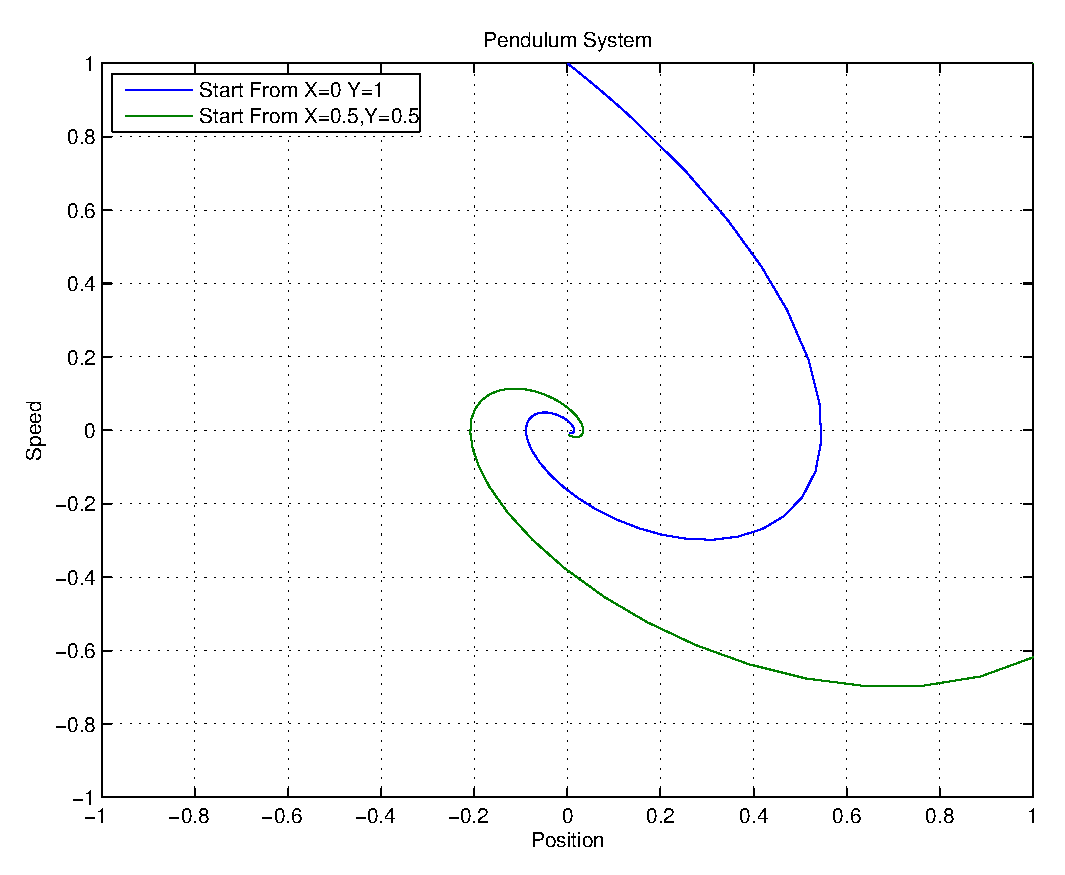
\includegraphics[height=0.4\textheight]{spring_damping}
\end{center}
\caption{damping perturbation onmass spring system}
\label{fig:dampmass}
\end{figure}

If ability of a dynamic system maintains its topology structure is structural stability.
To make characters more adaptive to environment and body change, motor controller should boost the structural stability of the motion.
Control effort should be prevent bifurcation.
\end{itemize}


\subsection{remarks on biological motor control}
Structural Stability is neglected in CMS research.
It is reasonable for natural animals to rely on structural stable autonomous system. 
In natural environment, perturbation and uncertainty are everywhere. In many cases, if neural system
can’t respond quickly enough, the better solution is to select a more structure stable motion primitives.

Structural Stability and Qualitative Idea provides a better explanation for some motion phenomena than quantitative theory like optimization and feedback shooting.
Qualitative Control Theory may help us understand the evolution of locomotion and neural Control.
Animals shift from the sea to the land. From quantitative computing viewport, the natural dynamics of the body and fluid environment are hard to predict or compute precisely. From the qualitative viewport, fluid is continuous
and uniform, the topology structure is very simple and stable, thus with little neural control fish can maintain its posture. On the other side, for human walking, although the rigid like
Environment can be calculated precisely, the topology structure is much more complex. 
Onthe phase plane, there exist many equilibrium points, the topology structure is more complex and unstable. 
The control system has to be more complex to control the more complex qualitative properties.

Qualitative theory can also help to explain another fact of biological motion system. 
Animals that live in similar environment and moves in a similar manner usually have similar body structure, in spite of their different position on evolution chain. 
This is because animals moving in a similar is based on the same motion primitive, similarity in body structure promise the topologial conjugacy.

This idea may help us to understand the body and environment effect in morphological computation theory. 
For specific environment, body evolves to provide us with a structural stable dynamic system, thus save lots of control effort for neural control.

We can also know motion primitives are not only defined by the body, it also defined by the environment, for motion in a specific environment, the topology should be fixed, thus the number of motion primitives is quite limited.


\section{Global Motor Invariant Control}
\subsection{CPG and Entrainment}
In nature, an animal's body and environment can be extremely complex. 
It leads to high dimensional manifolds with complicated topological structure, which provides many motion primitives for our use.
For CMS application, one question we want to ask is the so many motion primitives can be controlled with a simple method.

We propose that even there are many type of motion primitives, the type of attractor is limited. Basically there are only two types of attrator, limit circle and fix point.
Even the dimension of dynamic system maybe large, the dimension of the attrator is known. 
For fix point, its attractor is of dimension zero.
For limit circle, it is of dimension one.
Thus we can only focus on the type of attractor.



Biology Research suggested that the motor is mainly controlled by the Central Pattern Generator, which is a small autonomous network that generating rhythmic signals.
The idea of control motion by rhythmic signals can be modelled as entrainment \citep{Gonz'alez-Miranda2004}.
When coupling two oscillation system together, entrainment can happen when two system oscillator in synchronize. 
This effect will enhance the oscillation and also know as resonant. 




In previous section, we discussed two types of attractors: Fixed point and Limited Cycle. 
It is a still open question which type is more important and serve as the foundation as motor control\citep{Degallier2010}.
One idea limit circle is a necessary, fix point can be controlled with by 
(1) terminate a circle, 
(2)a different controller, 
(3)approximate by a limit circle with small amplitude or damping the limit circle, 
(4) change the limit circle into a fix point through by bifurcation. 



In this paper, 
\begin{itemize}
\HiItem Periodic behaviour is very common in biological systems. 
Besides the periodic motion in swimming and running, heart beating, wake and sleep also show periodic behaviour.
A periodic system has the potential to integrate with other bio system simulation to explore other motion features.

\HiItem Periodic motion has the same effect of terminated motion when the amplitude of limited circle is very small. 
For CMS research, both type of motion trajectory can be simulated with periodic motion.

\end{itemize}

\subsection{Neural Oscillator Stability}


Although it is difficult for neural system to carry out complex computation, it is easy to build oscillator structure with neurons. 
It only needs two neurons with mutual inhibitive property.
One extensively studied oscillation model is developed by \citet{neurooscillation}. 
The mathematical presentation is as follows:
\begin{eqnarray}
\tau_{1} \dot{s_{1}}&=&c-s_{1}-\beta l_{1}-\gamma [s_{2}]^{+}-\sum_{j}h_{j}[w_{j}]^{+}\\
\tau_{2} \dot{l_{1}}&=&[s_{1}]^{+}-l_{1}\\
\tau_{1} \dot{s_{2}}&=&c-s_{2}-\beta l_{2}-\gamma [s_{1}]^{-}-\sum_{j}h_{j}[w_{j}]^{-}\\
\tau_{2} \dot{l_{2}}&=&[s_{2}]^{+}-l_{2}\\
y_{i}&=&\mbox{max}(s_{i},0)\\
y_{o}&=&=[s_{1}]^{+}-[s_{2}]^{+}=y_{1}-y{2}
\label{eq:matsuta}
\end{eqnarray}

$c$,$\beta$,$\gamma$ are parameters of the oscillator,in our research are kept constant.
$\tau$ constrolls the oscilation frequency.







Matuoka oscillator is an autonomous oscillator; 
it can begin to oscillator without any control effort.
Figure ~\ref{fig:natural-oscilation} shows the natural oscillator output.
\begin{figure}[h]
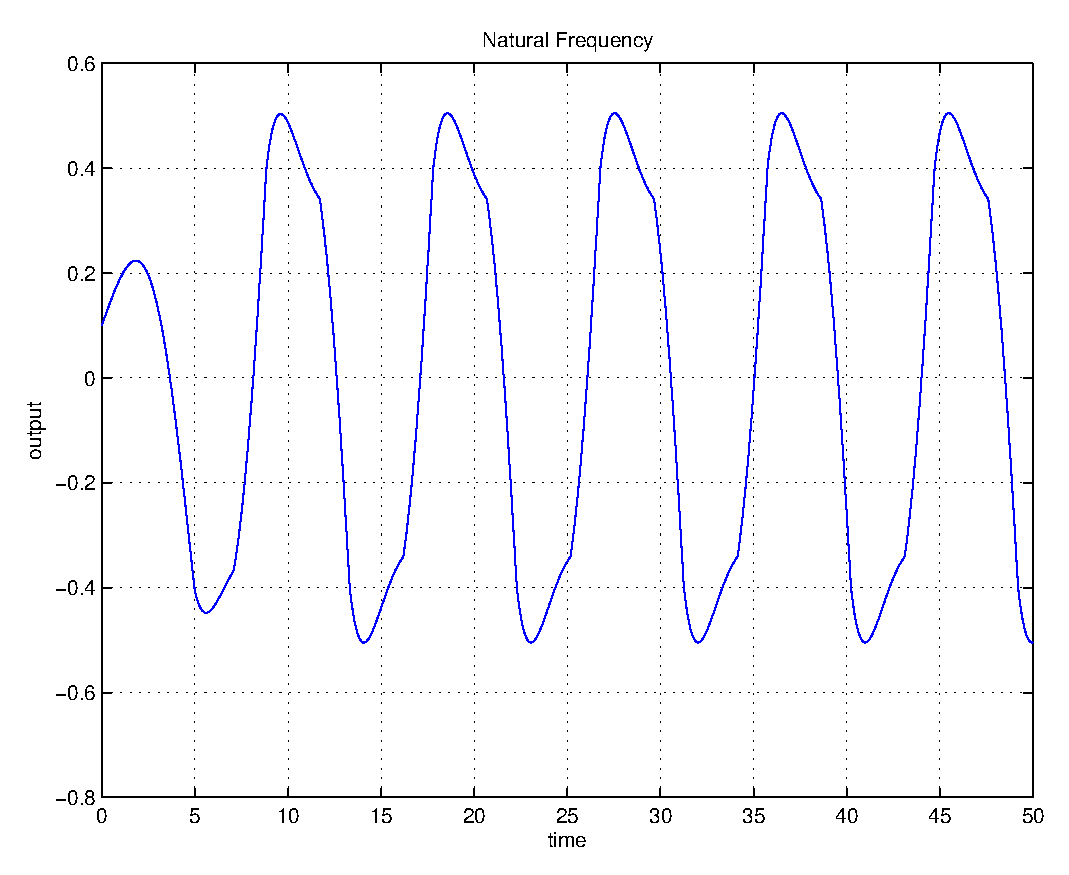
\includegraphics[height=0.4\textheight]{oscillation.eps}
\caption{Natural Oscillation}
\label{fig:natural-oscilation}
\end{figure}





It is also adaptive; entrainment behaviour can happen between one Matuoka oscillator and different oscillators. 
Figure \ref{fig:entraint-oscilation} shows the entrain oscillation,
where the oscillation of Matuoka oscillator synchronise with the input signal.
\begin{figure}[h]
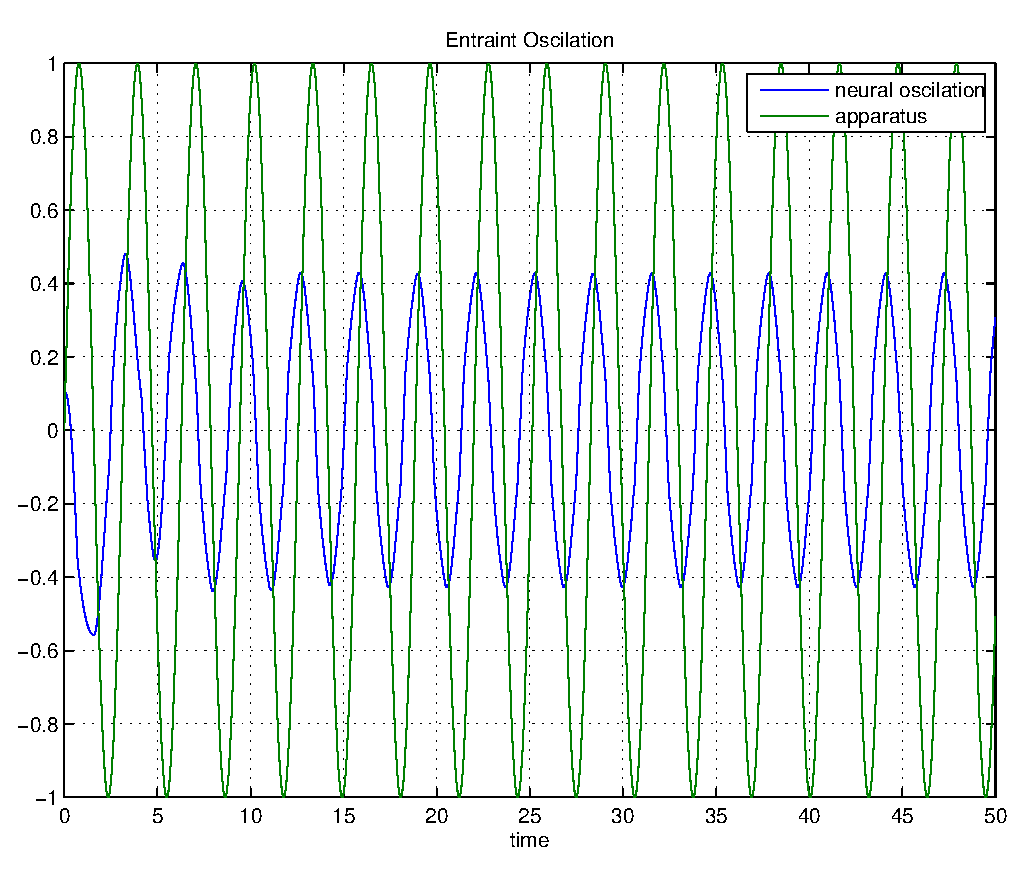
\includegraphics[height=0.4\textheight]{entraint_oscilation.eps}
\caption{Entrainment Oscillation}
\label{fig:entraint-oscilation}
\end{figure}

But because of the nonlinear properties, its behavior is not completely understood. 
Matsuta\citep{Matsuoka1987} explains the adaptive properties from the location of the roots of  characteristic equation. 
Wilimas\citep{Williamson1998} explains the properties in frequency domain.



In our research, we find some important properties of neural oscillator by empirical.

\begin{figure}
\begin{center}
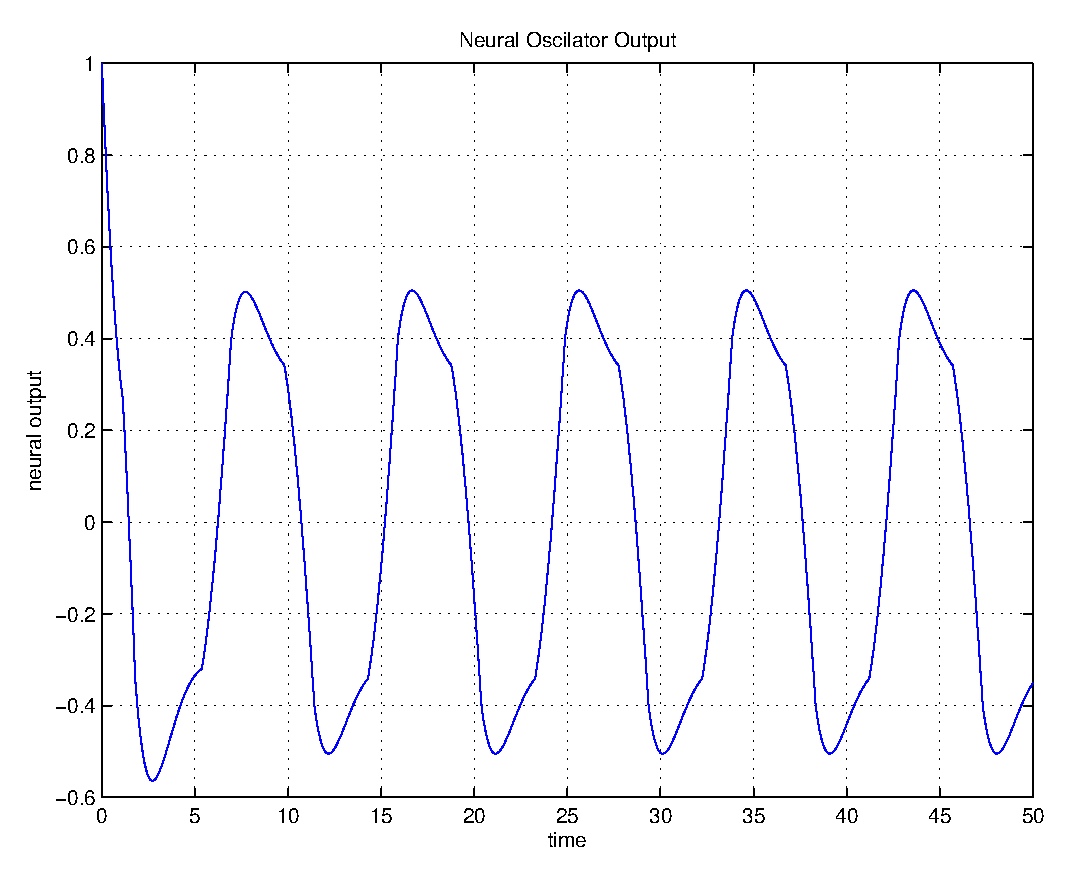
\includegraphics[height=0.5\textheight]{neuraloscilation1.eps}
\end{center}
\caption{The states of neural oscillator over Time}
\label{fig:oscilation}
\end{figure}

\begin{figure}
\begin{center}
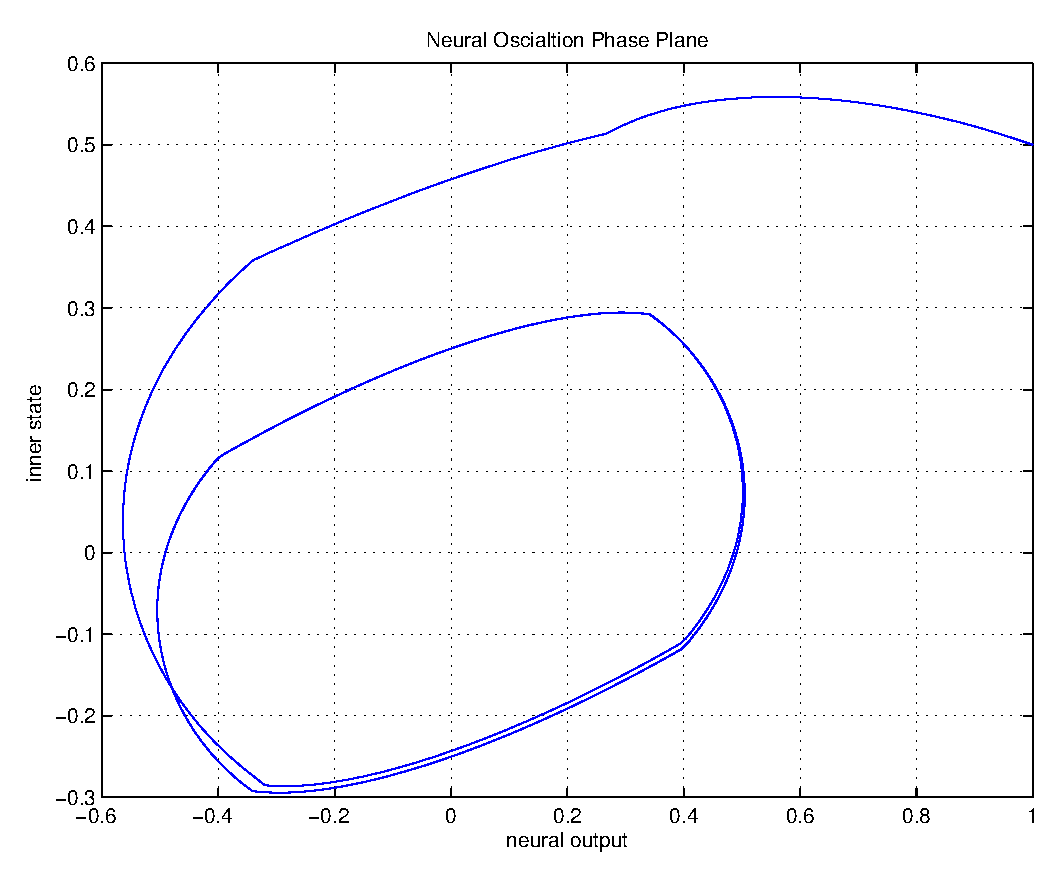
\includegraphics[height=0.5\textheight]{neural1phase.eps}
\end{center}
\caption{The phase portrait of Neural Oscillators}
\label{fig:oscilationphase}
\end{figure}

From our simulation, we investigate the topological structure.
Basically, neural oscillator shows three important properties:
\begin{itemize}
\item{Simple Topological Structure.}
The topology structure of neural oscillator is simple, 
it includes one  attractive limit circle and one fix repellor.
\item{Large Basin of Attraction.}
All the simulations we carried out converged to the same limited circle.
\item{Fast Converging Speed.}
In most of the case, the flow will converge to the limit circle within one period time.
\end{itemize}

Features above are shown in Figure ~\ref{fig:time_timeAttraction}.
\begin{figure}
\begin{center}
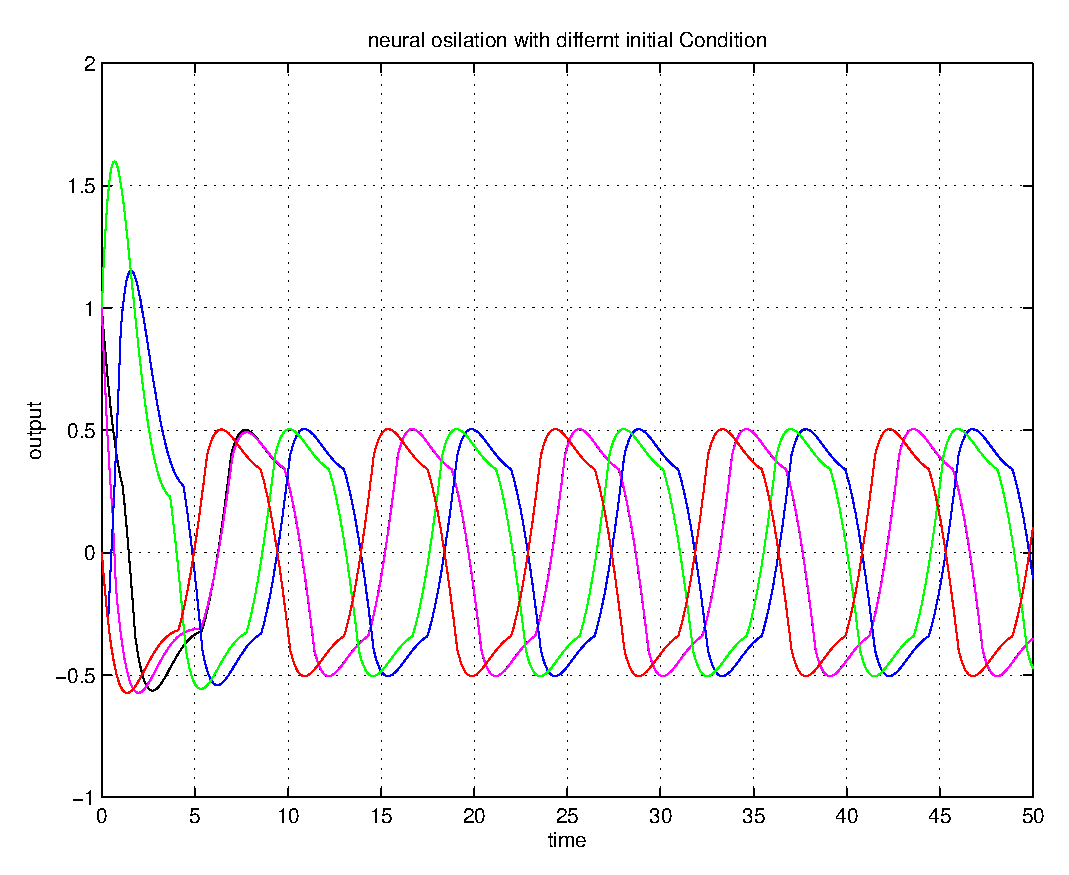
\includegraphics[height=0.4\textheight]{neural_attraction.eps}
\end{center}
\caption{Neural output with different initial position}
\label{fig:time_timeAttraction}
\end{figure}

\begin{figure}
\begin{center}
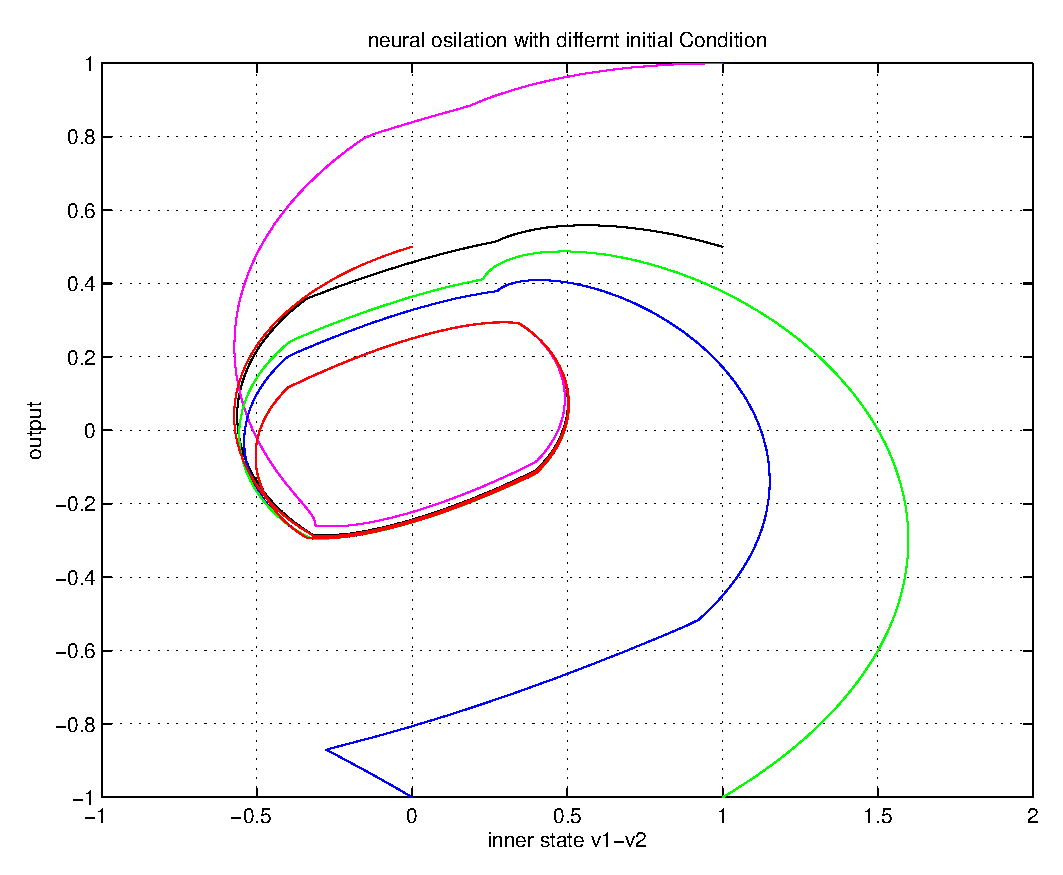
\includegraphics[height=0.4\textheight]{neural_attraction_phase.eps}
\end{center}
\caption{Phase plot of oscillation with different initial condition}
\label{fig:phase_attraction}
\end{figure}
 
The large area of basin of attraction means the final behaviour is totally determined by parameters. 
Initial condition will have no effects on the oscillator final output. 
Thus we treat matsuta oscilator as in a simple one input, one out put system, controlled by three parameter and input signal. 
we usually reformed equation ~\ref{eq:matsuta} in the simplified form
\begin{equation}
\label{eq:simplematsuta}
\uout=S_{[\hin,\hout,\tau]}(\uin)
\end{equation}
where $\uin=\sum_{j}h_{j}[w_{j}]=hw$,$\uout=\hout y_{o}$





The converging speed can be seen as quick recovery ability.
When an impulse perturbation happens, it will recover in one period time.


\section{Example:Maintain Bouncing Height}

Bouncing ball is system ball bouncing by moving a pedal, a system with simple dynamic but difficult to control with optimizaiton or pd. 
While this example capture the complexity of human interatction with the environment and object. 
And can be the basic model for many motion tasks.

We show in this example how neural oscillator can turn the bouncing ball system into motion primitive.
\subsection*{Dynamics}
Hybrid dynamics, in incoperate two phase, 
 

\begin{align}
\ddot{q}&=-g&\mathrm{if}\,\,q &> 0\,\,\mathrm{(free\,\,flying)} \nonumber\\
\dot{q}^{+}_{\mathrm{ball}} - \dot{q}^{+}_{\mathrm{paddle}} &=  \epsilon(\dot{q}^{-}_{\mathrm{ball}} - \dot{q}^{-}_{\mathrm{paddle}})&\mathrm{if}\,\,q &\leq 0\,\,\mathrm{(paddle\,\,strike)}\nonumber
\end{align}

Basically, the ball will continue bouncing with smaller height,as show in Figure~\ref{fig:bborg}.

\begin{figure}[h]
\begin{center}
	\subfigure[state plot]
	{
	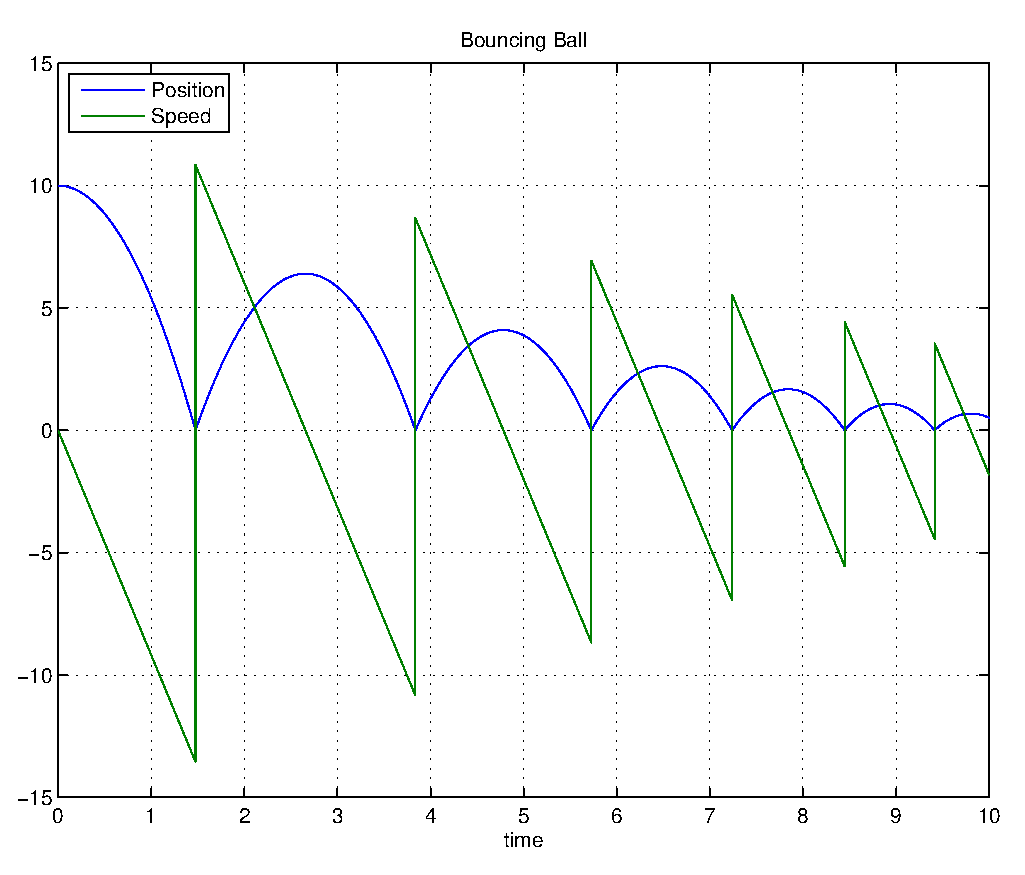
\includegraphics[width=0.45\textwidth]{bouncing_ball}
	\label{fig:bb}
	}
	\subfigure[Phase Plane]
	{
	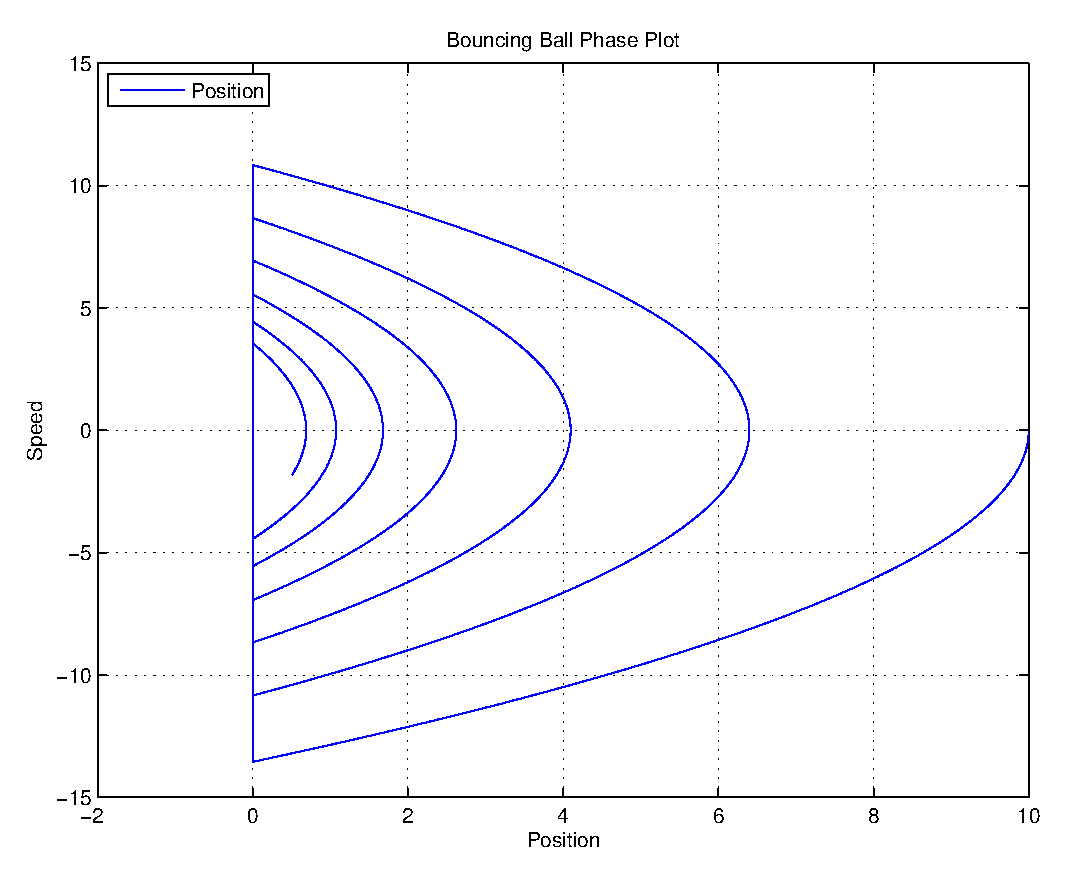
\includegraphics[width=0.45\textwidth]{bouncing_ball_phaseplot}
	\label{fig:bbp}
	}
	
\end{center}
\caption{Original Bourncing Ball System}
\label{fig:bborg}
\end{figure}



\subsection*{Emergence of Limit Cycle}
couple with neural oscillator boucing we get an limit circle
The input of neural oscillator is the velocity $\uin=\dot{q}_{ball}$, the output of neural oscillator  drive the pedal position $q_{pedal}=\uout$.
An limit circle emerge as the result of entrainment.
As show in figure drop from different position, all the ball will bouncing a about the same height of 5,as show in Figure~\ref{fig:bb_attractive_circle}

\begin{figure}[h]
\begin{center}
	\subfigure[state plot]
	{
	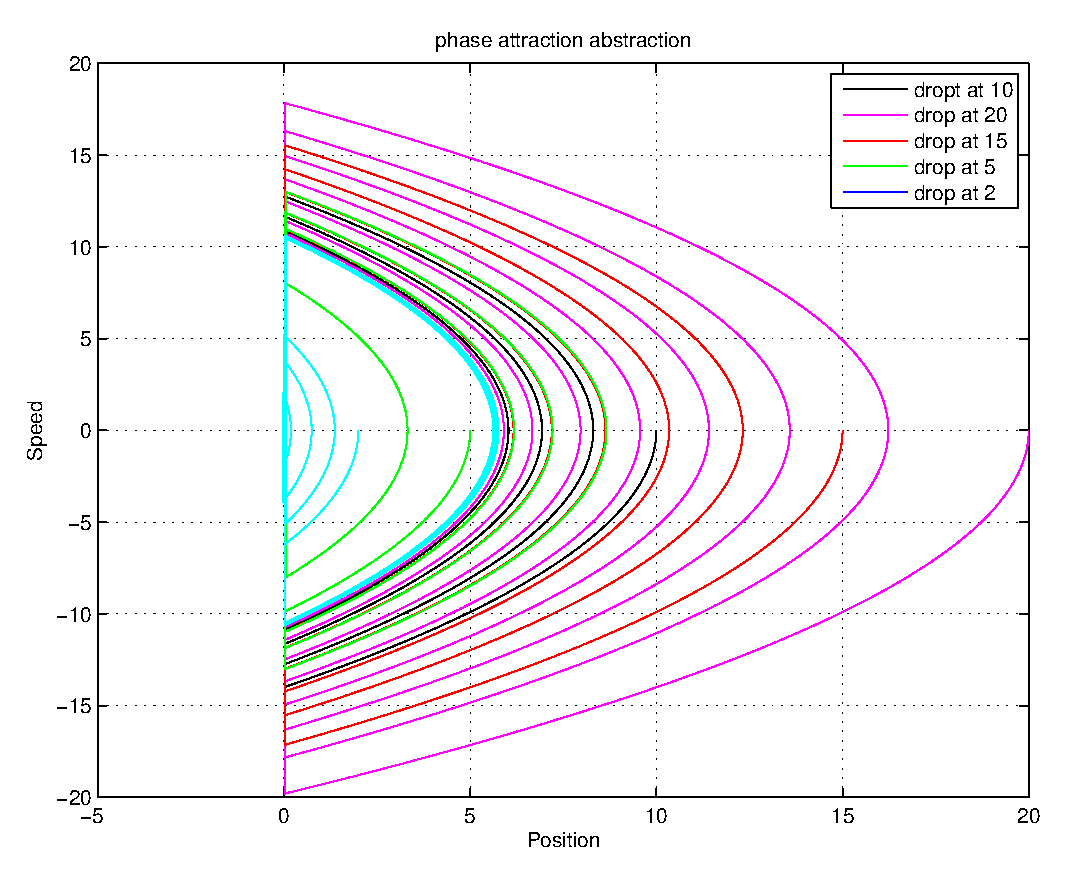
\includegraphics[width=0.45\textwidth]{bb_ms_os_attraction_phase}
	\label{fig:bb_attractive_entraint}
	}
	\subfigure[Phase Plane]
	{
	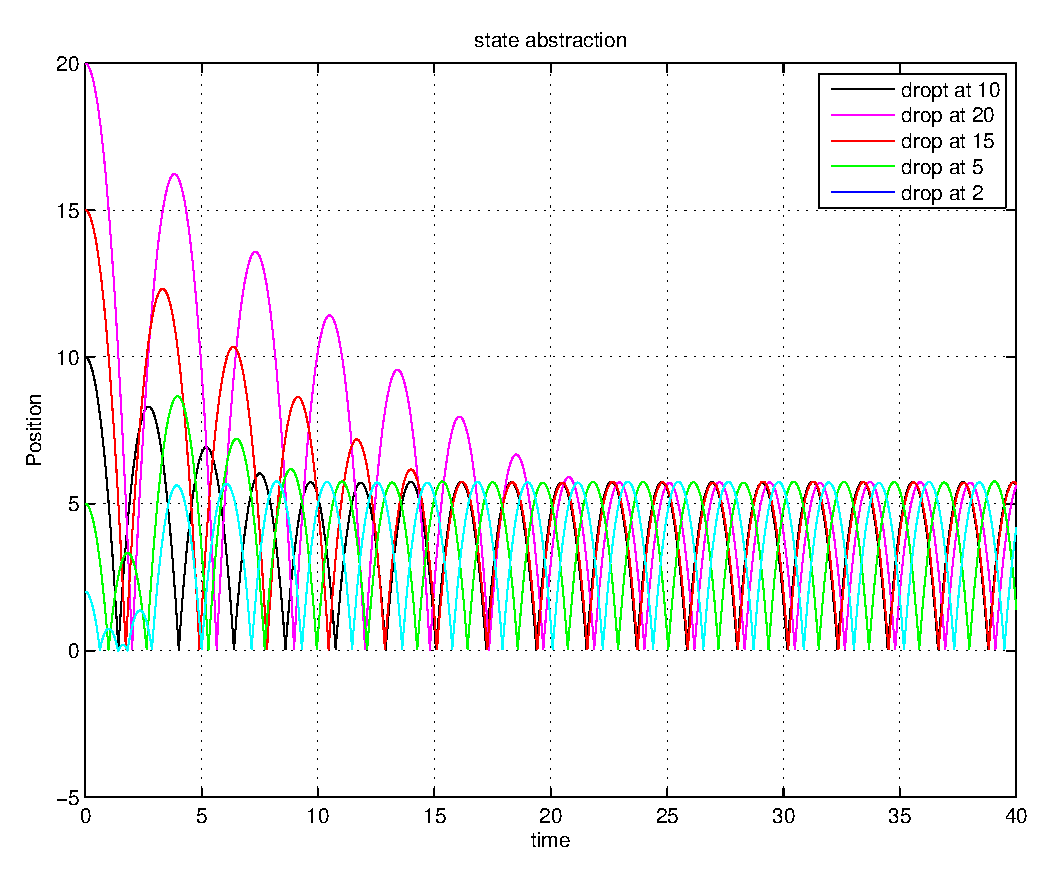
\includegraphics[width=0.45\textwidth]{bb_ms_os_StateTimeAttraction}
	\label{fig:bb_attractive_entraint_time}
	}
	
\end{center}
\caption{Attractive Limited Circle}
\label{fig:bb_attractive_circle}
\end{figure}

\chapter{LOCAL MOTOR INVARIANT}
\label{chap:li}

\nomenclature[f1]{$G$}{A Lie Group}
\nomenclature[f2]{$g_a$}{an element in Lie Group $G$ with parameter $a$}
\nomenclature[f3]{$I(x)$}{Invariant Function of $x$}
\nomenclature[f4]{$\ep$}{The parameter of a lie group element}
\graphicspath{{LocalInvariant/LocalInvariantFigs/EPS/}{LocalInvariant/LocalInvariantFigs/}}
It is not enough that animals are able to maintain the global motor invariant.
For a fish, preserving \emph{Global Motor Invariant}  means the swimming is stable and can be sustained.
However,  a fish also needs to adjust the speed and direction during swimming, which is of crucial importance for survival.
In real-life, animal can adapt motion primitives according to its purpose precisely.
In this chapter, we will develop the control strategies for tweaking motion patterns according to the motion purposes.

It is important to remember that such tweaking strategies are also constrained by the computation and memory capacity of the neural system, and should explore natural dynamics as the basic motion primitive theory. 
For \cms, it is of no meaning developing walking pattern by exploring natural dynamics but using optimization to adjust the walking speed. 
To meet such requirements, \moit\ adopted different ideas.

At first, when tweaking motion patterns, stability should not be violated. 
As stated in the previous chapter, a topological conjugation (one-one continuous invertible mapping)maintains the topology thus maintains the qualitative stability. Thus the ``tweaking'' action should be a topology conjugation. In an alternative perspective, such operations form a group and permit a combination operation. 

According to Group Theory, this means if two tweaking actions preserve the stability separately, the combination of the two actions also preserve the stability.
The space of topology conjugation is very large.
Currently, \moit\ only investigates a subset called \emph{The Lie Transformation Group} that is supported by the biological research studies and can be calculated efficiently.
The selected groups can be divided into orthodox subgroups, each of which is continuous and can be parameterized by one parameter.
In \cms, such parameters are closely related to motion purposes such as walking speed or swimming direction.

From the dynamic perspective, ``tweaking''  should also explore natural dynamics (passive based) as primitives.
Methods adopted in \moit\ belong to  a popular passive-based control principle, which carries many names: Controlled Symmetry, Controlled Lagrange, or Potential Shaping.
Different names reflect the fact that this method can be developed through different ways.
Roughly speaking, the original dynamic system is transformed according to motion purpose, the kinematics is untouched and control is applied by modifying the potential energy.
Such methods suit biological actuators like muscles and are also computationally efficient:
Closed form formula are developed for converting tweaking parameters to control effort.

This chapter is laid out in this way:
Section~\ref{sec:groupandsymmetry} introduces the basic idea of group and symmetry from intuitive geometry examples to more abstract algebraic formulation. Section~\ref{sec:liecontrol} investigates application of the Controlled Lagrange Method.
At last an example is provided in Section~\ref{sec:symball} to illustrate the idea.

In theory the ideas of group and invariant are closely related, like the two sides of a coin.
Group are the transformations which keep certain property invariant.
When searching for the group transformation, the invariant property is also determined.

In Motor Invariant Theory, the quantitative properties that are  preserved during group transformation are called \emph{Local Motor Invariant}.







\section{Group and Symmetry}
\label{sec:groupandsymmetry}
%To make motions realistic, some natural looking features should also be preserved.
%Some features of motions such as smoothness or energy efficient are quantitative.
%\cms research should provide a framework preserving feature.
%Another question mission is animals can finish motion tasks require high accuracy.
%
%These are the motivations for the development of \emph{Local Motor Invariant}.
%Local Motor Invariants are quantitative properties of motions, the idea of invariant preserving are abstracted as the ``Symmetry'' and Group theory.
%Features are modelled as symmetrical functions, while feature preserving actions form a group.
%From dynamic perspective, motions are solutions to dynamic equations.
%The actions transform one motion to another close related to the Lie Group Theory for differential equations\citep{olver1986applications}.
%
%The introduction of Lie Group not only provides a powerful mathematical tools for modelling the symmetry property, but also provides an idea to simplify the solving the dynamics.



For the more traditional geometrical perspective, ``Symmetry''  means a geometry is the same after certain transformation.
For example, a square remains the same shape after  $90$ degree clockwise rotation, as shown in Figure~\ref{fig:symsquare}.
\begin{figure}[!htbp]
  	\begin{center}
   	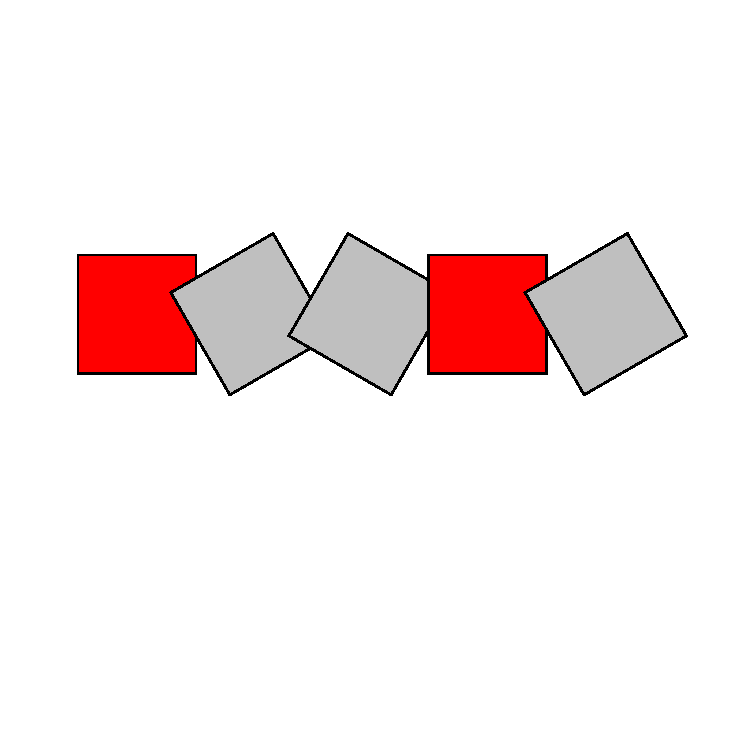
\includegraphics[width=0.5\textwidth]{SquareRotate}
	\end{center}
	\caption{Symmetry of The Square}
    \label{fig:symsquare}
\end{figure}

Actions that preserve the square shape can be combined.
For example, if the action of $90$ degree clockwise rotation preserves the shape, then the action of rotating twice, i.e., $180$ degree clockwise rotation also preserves the shape.

All the actions that can preserve the symmetry form a group $G$.
A group has the following properties.
\begin{enumerate}
\item For any $g_a,g_b$ in $G$, \,$g_a*g_b$\, belongs to $G$. (The operation ``$*$'' is closed).

\item For any \,$g_a,g_b,g_c\in G$, \,$(g_a*g_b)*g_c=g_a*(g_b*g_c)$. \,(Associativity of the operation).

\item There is an element $e\in G$ such that \,$g_a*e=e*g_a=g_a$\, for any \,$g_a\in G$. (Existence of identity element).

\item For any \,$g_a\in G$\, there exists an element $g_h$ such that \,$g_a*g_h=g_h*g_a=e$. \,(Existence of inverses).
\end{enumerate}

For the square example, all the actions preserve the square shape form the group $G$.
$g_1$ is  $90$ degree clockwise rotation, identity element $e$ is the action of no rotation,
$g_2=g_1*g_1$ is the action of rotating $90$ degree clockwise twice.
Since $g_2$ preserves symmetry, $g_2$ is an element of the group $G$, 


From the algebraic perspective, ``Symmetry'' means the value of function is invariant after transformation.
For a function $I(x)$,
the group transformation is define by $\tilde{x}=g_a(x)$.
By symmetry, we mean $I(x)=I(\tilde{x})$.
$I(x)$ is an invariant function of group $G$.


Note that  shapes invariant by actions in $G$  are not unique.
Many shapes are invariant, and their combinations are also invariant, as shown in Figure~\ref{fig:SymmetrySpace}. 
In the algebraic sense,  invariant functions of group $G$ form a space, the invariant space $I^G$.


\begin{figure}[!htbp]
  \begin{center}
    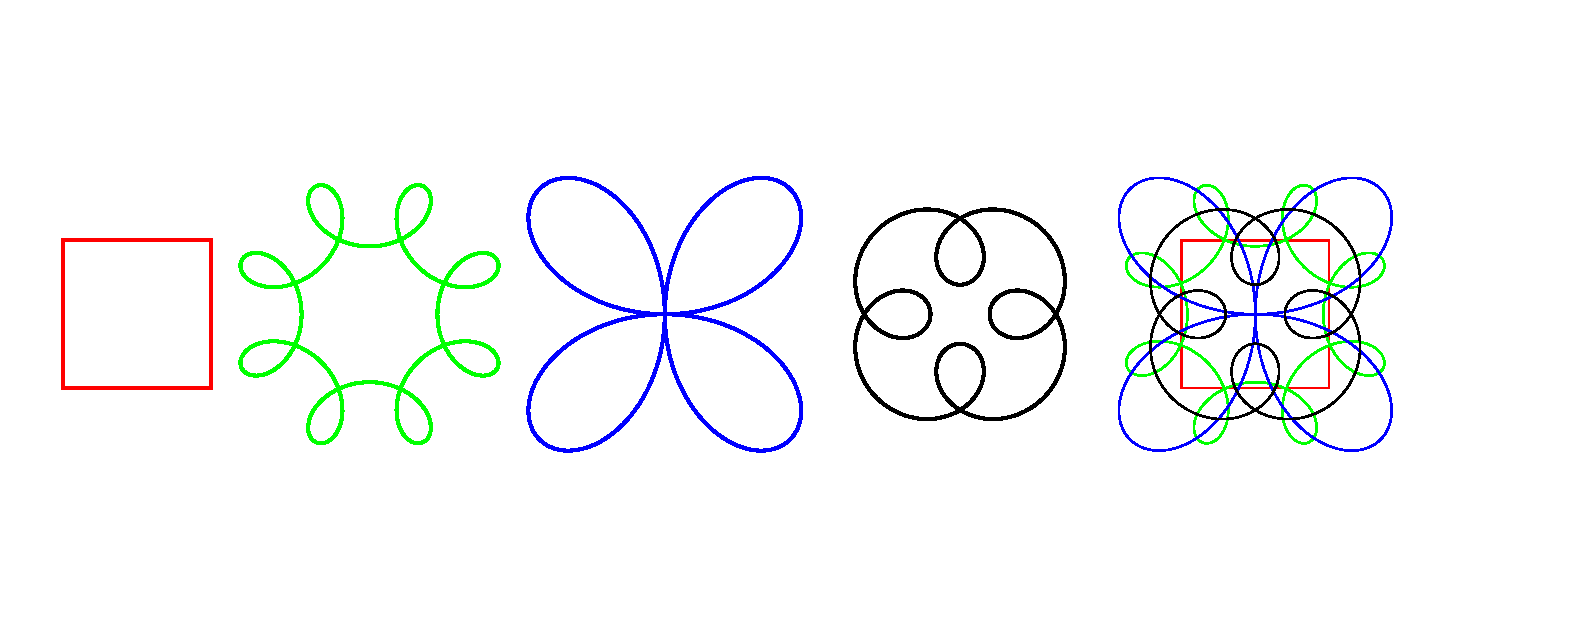
\includegraphics[width=0.7\textwidth]{ShapeCombination}
    \caption{Two invariant Shapes and the invariant combination}
    \label{fig:SymmetrySpace}
\end{center}
\end{figure}

\subsection{Lie Group and Differential Equation}
Physically-based motions are usually described by differential equations, and motion is the solution of the equation.
Same as the square shape, there are also symmetry groups that keep the differential equations invariant.
An important property of such a group  is that its elements can transform the solution of differential equations from one into another\citep{olver1986applications}.
For \cms, this property  can potentially help reduce computational burden: new motions can be achieved through applying  transformation to the dynamic equations of motion primitives.




In mathematical theory, \emph{Lie Group} is continuous group, which is also a manifold.
Since it is a manifold, coordinate system can be assigned to a Lie Group and each elements can be parameterized.
For example, the symmetry rotation group of square is discrete, while symmetry group of circle is continuous.
For the symmetry group of the circle, each element can be parameterize by the the rotation angle.
In the following discussions,  $\ep$ is the parameter of a element $g$ in the group $G$.

Theory of Lie group comes from the study of differential equations.
For the differential equation in Equation~\ref{eq:difforg}.
\begin{equation}
\label{eq:difforg}
\dot{\state}=F(\state)
\end{equation}
Invariant function $I$ can be defined as:
\[
I(t,\state,\dot{\state})=F(\state)-\dot{\state}
\]
Solutions of the differential equation are the kernel of the invariant function $I$ :
 \[
 I(t,\state,\dot{\state})=0
 \]
 
 
The group transformation will act on all the variables of the invariant function.
Therefore $t$, $\state$ and $\dot{\state}$ are all transformed.
\[
(t,\state,\dot{\state}) \mapsto (\tilde{t},\tilde{\state},\dot{\tilde{\state}})
\]
If the group $G$ is symmetrical, then value of the  function $I$ will be invariant.
Therefore  the kernel is transformed into kernel, and the transformed variables are still solutions to the original differential equations. 
\[
I(t,\state,\dot{\state})=I(\tilde{t},\tilde{\state},\dot{\tilde{\state}})=0
\]


Note that the $\dot{\state}$ is not independent which depends on the $t$ and $\state$,
\[
\dot{\tilde{\state}}=\frac{d \tilde{\state} }{d \tilde{t}}
\]
From the geometrical perspective, it is not easy to present  the transformation of $t$.
Instead, we define two actions on the state space and tangent space.
In the state space, we define the  action $g$ that transforms the state. 
\[
g(\state)=\tilde{\state}
\]
In the tangent space, we define the \emph{lift action} $Tg$ 
\[
Tg(\dot{\state})=\dot{\tilde{\state}}
\]

$Tg$ can be worked out by formatting the derivatives in the original coordinate system.
For example, the translation $g_{\ep}$ 
\[
(x,y)\mapsto (x+\ep,y+\ep)
\]
$Tg_{\ep}$ is
\[
(\dot{x},\dot{y}) \mapsto (\dot{x},\dot{y})
\]
$Tg$ is the identity element $e$.


In the general cases, $g$ transforms Equation~\ref{eq:difforg} into Equation~\ref{eq:trdiff}
\begin{equation}
\label{eq:trdiff}
Tg(\dot{\state})=F(g(\state))
\end{equation}
If $g$ is symmetrical, Equation~\ref{eq:difforg} and Equation~\ref{eq:trdiff} are equivalent







 	
For example, 
The scaling action is applied to the state space of the mass spring system of Equation~\ref{eq:stateform}. 
\[
\tilde{\state}=g_{\ep}(\state)=[\ep q, \ep \qd ]
\]
then the lift action is
\[
\tilde{\state}=Tg_{\ep}(\state)=[\ep \qd, \ep \ddot{q}]
\]



by substitution $\state \mapsto \tilde{\state}$, the original system becomes
\[ 
\dot{\tilde{\state}}=
\left[ 
\begin{array}{cc}
0 &1\\
-1 &0 
\end{array}
\right]\tilde{\state}
\]
which is 
\begin{equation}
\label{eq:tranmas} 
\ep \dot{\state}=
\left[ 
\begin{array}{cc}
0 &1\\
-1 &0 
\end{array}
\right]\ep \state
\end{equation}

Equation ~\ref{eq:tranmas} is equivalent to  Equation~\ref{eq:stateform}.
If $\state(t)$ is a solution, so is $\tilde{\state}(t)$.

To verify the group property. define $*$ as:
\[
g_{\ep_1}*g_{\ep_2}(\state)=[\ep_1 \ep_2 q, \ep_1 \ep_2 \qd]
\]

The inverse is:
\[
g_{\ep}^{-1}=g_{\frac{1}{\ep}} \;\ep \in R^+
\]

\begin{mydef}
For a group $G$, the invariant function of state $I(\state)$ is called a \emph{local motion invariant} of $G$. 
\end{mydef}

Invariant functions $I(\state)$ has important  meaning in dynamics. 
According  to \textbf{Noether's Theorem}, each $I(\state)$ corresponds to a conservative law. 


\section{Lie Group and Controlled Lagrange}
\label{sec:liecontrol}
It is not enough for animals  only to  explore symmetry groups of natural dynamics for motion adaptation.
For a dynamic system, the symmetry group is quite restricted.  
Working out the symmetry group might be a non-trivial task.
In real-life, animals usually exert control effort during motion adaptations.

\moit\ theory proposes the idea that control effort can make a non symmetrical group become symmetrical, and introduce the \emph{Controlled Lagrange} technique.
Based on biological research\citep{flash2007affine}, some simple groups are selected the symmetry group for motor control.
When such group is applied to the dynamic system, control efforts are applied to ensure the symmetry.


Usually a dynamic system is represented as by Euler-Lagrange Equation~\ref{eq:uncontrolled_euler_lagrange}\citep{Goldstein2002}.
\begin{equation}
\frac{d}{dt} \frac{\partial L}{\partial \qd} - \frac{\partial L}{\partial q} = 0
\label{eq:uncontrolled_euler_lagrange}
\end{equation}

where $L=K-V$, $L$ is the Lagrange, $K$ is the kinetic energy, $V$ is the potential energy, $q$ is the generalized coordinates, and $\qd$ is the generalized velocity.

By applying the group transformation $g$, both the generalized coordinates and generalized velocity will be changed:
\[
g(\state)=\tilde{\state}=[\tilde{q}, \dot{\tilde{q}}]
\]
The Euler-Lagrange equation for the transformed dynamic system is described by Equation~\ref{eq:liegroup_euler_lagrange}.
If control is applied, the Euler-Lagrange equation of the controlled dynamics is described by Equation~\ref{eq:controlled_euler_lagrange}. 
If symmetry is persevered, the two equation should be equivalent.
Then symmetry control input $\ulocal$ can be calculated by comparing the two equations.
\begin{align}
\frac{d}{dt} \frac{\partial L}{\partial \dot{\tilde{q}}} - \frac{\partial L}{\partial \tilde{q} }&=0,\label{eq:liegroup_euler_lagrange}\\
\frac{d}{dt} \frac{\partial L}{\partial \qd} - \frac{\partial L}{\partial q}&=\ulocal. \label{eq:controlled_euler_lagrange}
\end{align}

When the two equations are equivalent, their Lagrange $L$, Kinetic Energy $K$ and potential energy $V$ should be the same or of the same scale factor.
Thus in theory, two strategies exist and will result in two different $\ulocal$:
we can calibrate the kinetic by scaling and apply control effort to compensate the difference in potential energy, or calibrate potential energy and compensate the kinetic energy.
\moit\ adopts the potential shaping strategy, for it is computational efficient and suitable for muscle like biological actuators.
As a special case, potential energy shaping for homogeneous group or affine group promises a close form formulation.
Several groups and their potential shaping control effort are as below:



\subsection*{ Offset Action}
Offset actions  modify the generalized coordinate $q$ by a constant, while speed and time remain unchanged.
Given the offset parameter $\ep$, the mapping will be in the following form:
\[
(t,q,\qd) \mapsto (t,q+\ep,\qd)
\]

The corresponding state transformation and lift action are
\begin{align}
\goff(\state) &= [q+\ep,\qd] \\
T\goff(\dot{\state})&=\dot{\state}=[\qd,\qdd]
\end{align}


On the phase plot,  the configuration $q$ is usually represented by the horizontal axis, and the generalized speed $\dot{q}$ is represented by the vertical axis.
From the geometrical perspective, offset actions will move the phase portrait horizontally as shown in Figure~\ref{fig:goff}.

\begin{figure}[!htbp]
  \begin{center}
      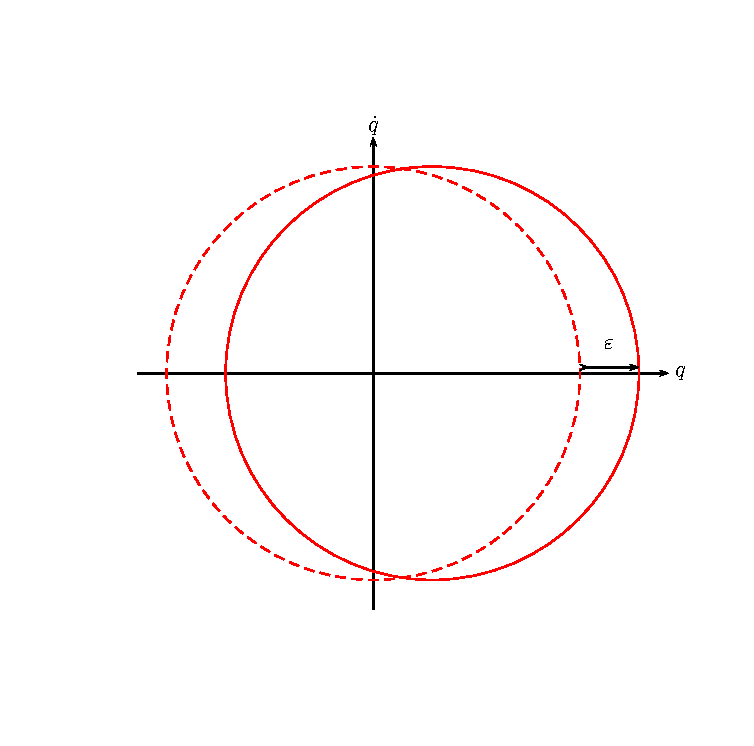
\includegraphics[width=0.5\textwidth]{OffsetAction}
    \caption{Offset Action}
    \label{fig:goff}
\end{center}
\end{figure}

Substituting the transformed $q$ and $\qd$ into Equation~\ref{eq:liegroup_euler_lagrange} and Equation~\ref{eq:controlled_euler_lagrange},
the control input  can be worked out in the following closed form formula:
\begin{equation}
\ulocal(q) = \frac{\partial}{\partial q} \left(V(q)-V(\tilde{q}) \right).
\end{equation}

Taking the mass spring system of Equation~\ref{eq:mass-spring} as an example, the transformed equation  and control equation are as follows.
\begin{align}
\ddot{\tilde{q}}+\tilde{q}-\ep&=0 \nonumber \\
\ddot{q}+q&=\ulocal \nonumber
\end{align}
By comparing the two equations, we work out that:
\[
\ulocal(q)=\ep
\]




\subsection*{Time Scaling}

%g_st(q,dot{q})=(q,st*dot{q})
Time scaling actions divide the time variable by a factor $\ep$.
The generalized coordinates are kept unchanged, and the generalized speed will be multiplied by $\ep$.
For the action of parameter $\ep$, the action mapping is: 


\[
(t,q,\qd) \mapsto (\frac{t}{\ep},q,\ep \qd)
\]

The corresponding state transformation and lift action are
\begin{align}
\gts(\state)&=[q,\ep \qd] \nonumber \\
T\gts(\dot{\state})&=[\ep \qd,\ep^2 \ddot{q}]\nonumber
\end{align}

From a geometrical perspective, time scaling will stretch the phase portrait vertically, as shown in Figure~\ref{fig:gts}.
\begin{figure}[!htbp]
  \begin{center}
    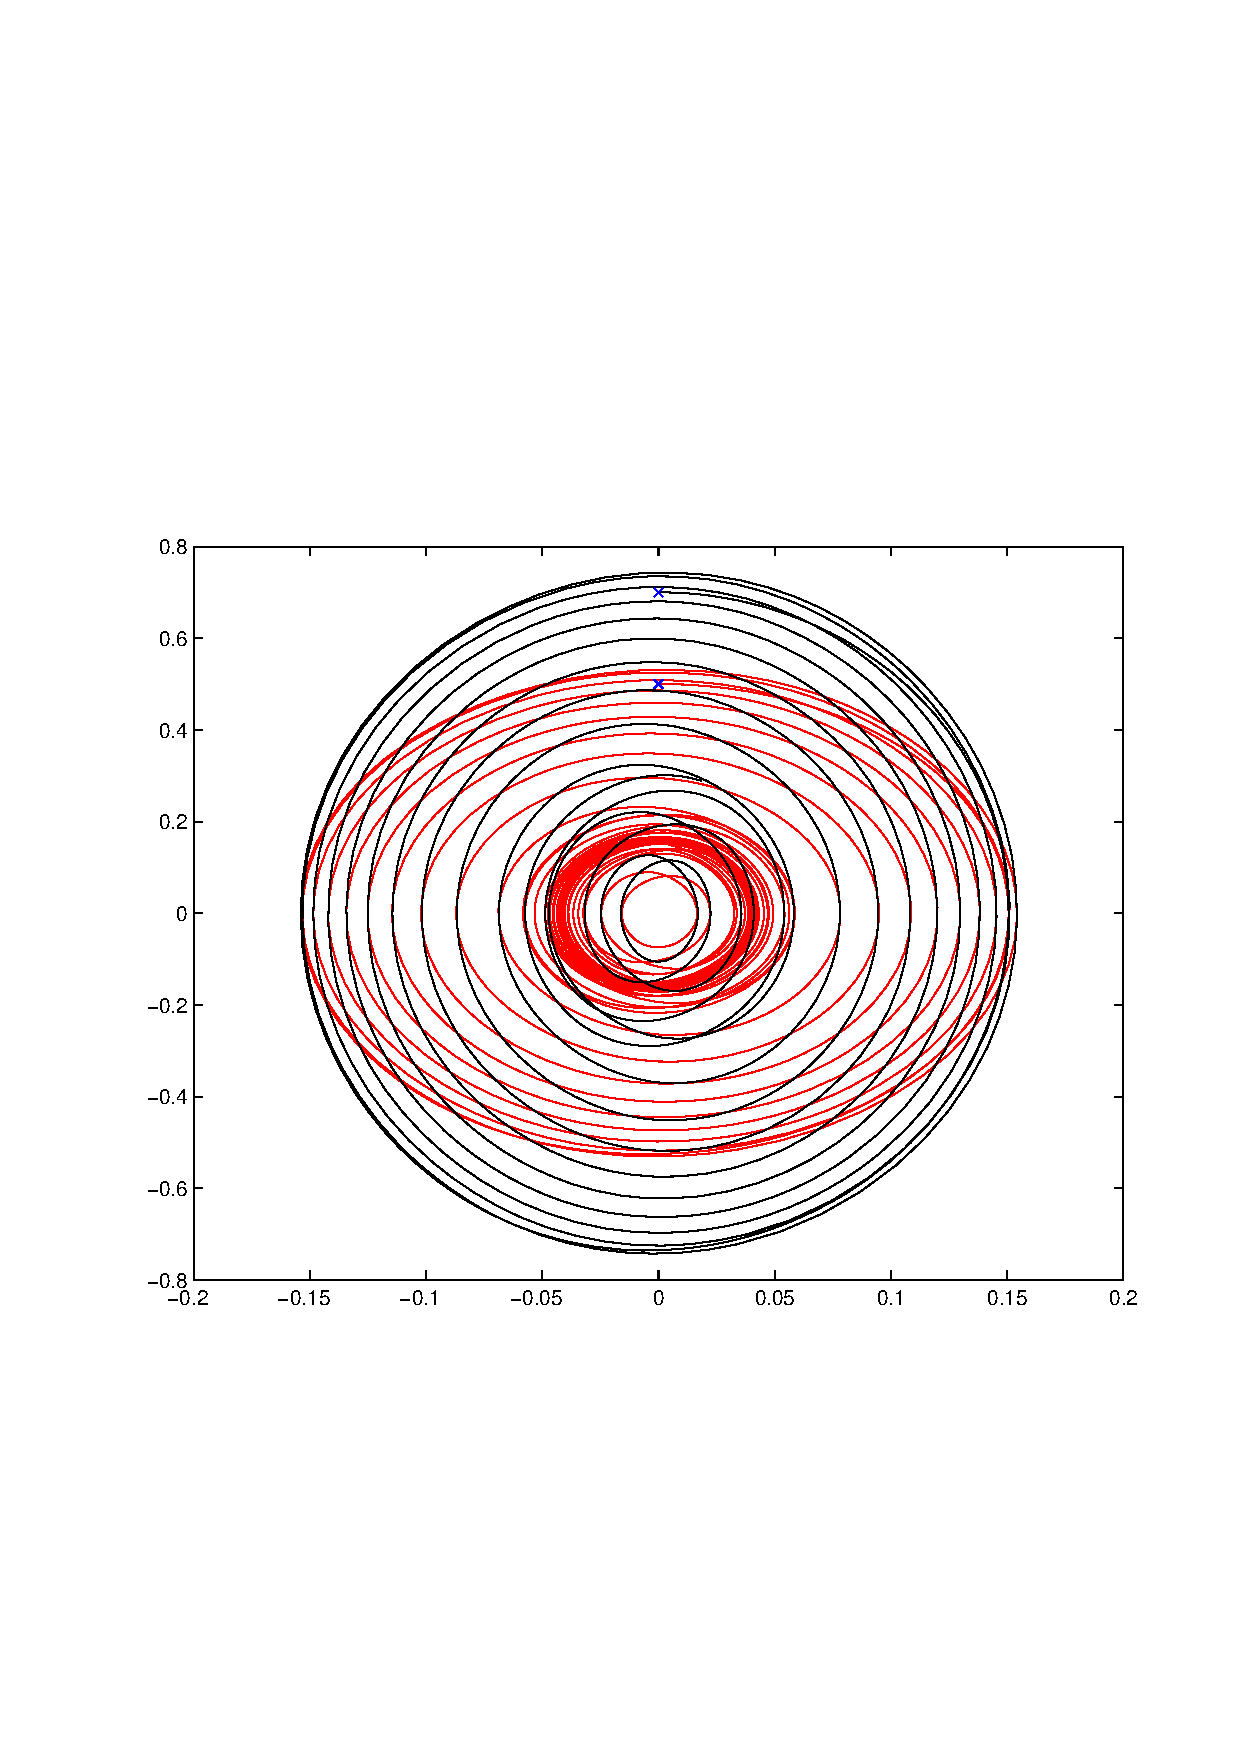
\includegraphics[width=0.5\textwidth]{TimeScaling}
	 \caption{Time Scaling Action}
    \label{fig:gts}
\end{center}
\end{figure}

The control input can be worked out in the same manner as offset actions.
There is also a closed form formula for control input.
\begin{equation}
\ulocal(q) = (1-\ep^2) \frac{\partial V(q)}{\partial q}.
\end{equation}

Again, taking the mass spring system of Equation \ref{eq:mass-spring} as an example, the transformed and controlled equations are

\begin{align}
\frac{\ddot{\tilde{q}}}{\ep^2}+\tilde{q}&=0 \nonumber \\
\ddot{q}+q&=\ulocal \nonumber
\end{align}
The local control input is:
\[
\ulocal=(1-\ep^2)q
\]




\subsection*{Energy Scaling}
For the  dynamic system of the conservative field,
the energy is preserved in motion and different motions are characterized by their energy.
For such a system, motion can be adapted by modifying the energy of the dynamic system.

Energy Scaling action is introduced to adapt motions.
The scaling transformation has the following property:
\[
E(\tilde{\state})=\ep^2 E(\state)
\]
where $E$ is the energy, defined as $E(\state)=K+V$,  $K$ is the kinetic energy, and $V$ is the potential energy.

Further suppose that both the potential and kinetic energy are transformed uniformly.
\begin{align}
K(\tilde{\state})=\ep^2 K(\state) \nonumber\\
V(\tilde{\state})=\ep^2 V(\state) \nonumber
\end{align}
When mass inertia matrix is constant,  the energy scaling transformation is linear as follows:
\[
(t,q,\qd ) \mapsto ( \frac{f(\ep)}{\ep}t ,f(\ep)q,\ep\qd)
\]
$f(\ep)$ is a function of $\ep$, which is determined by the conservative field.
Geometrically, an energy scaling action enlarges the phase portrait,as shown in Figure~\ref{fig:gen}.
\begin{figure}[!htbp]
  \begin{center}
      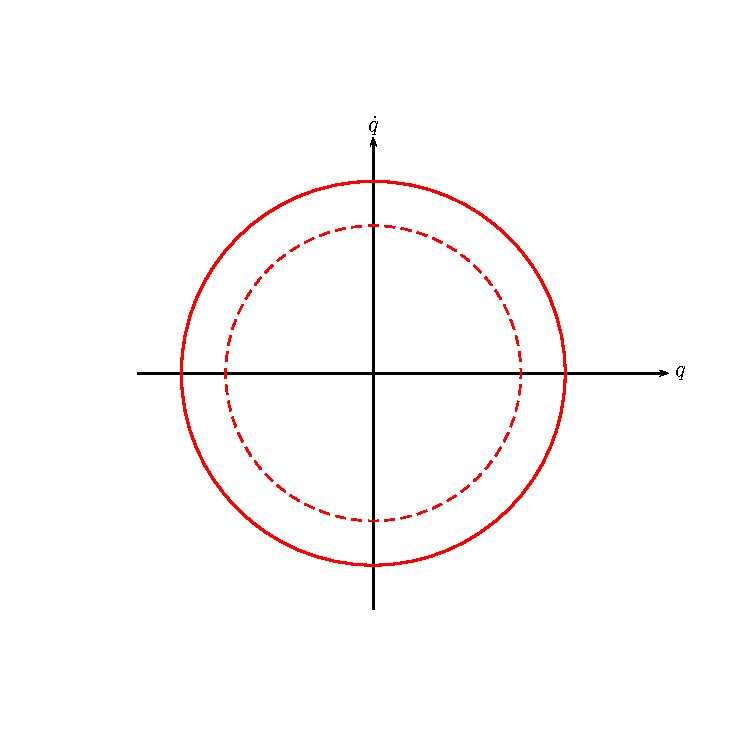
\includegraphics[width=0.5\textwidth]{EnergyScaling}
    \caption{Energy Scaling Action}
    \label{fig:gen}
\end{center}
\end{figure}

The corresponding  state transformation and lift action are:
\begin{align}
\gen(\state)&=(f(\ep) q,\ep \dot{q}) \nonumber\\
T\gen(\dot{\state})&=(\ep \dot{q},\frac{\ep^2}{f(\ep)}\qdd)
\end{align}

$\ulocal$ can by worked out in the same manner as the above actions.
Rather than write down the closed form formula, the thesis prefers an alternative process.
Energy Scaling can be seen as a combined action of two actions: scaling the generalized coordinates and scaling the time variable.
Separate formula can be developed for two actions independently.
This principle generates modular code structure.




The mass spring system of Equation\ref{eq:mass-spring} is selected again as an example.
 For the mass spring system, Energy is defined as~$E=\frac{1}{2}(q^2+\qd^2)$.
 If the energy is scaled up by $\ep^2$,  the potential energy is scaled up by $\ep^2$.
 Because $V= \frac{1}{2}q^2$, and $\ep^2 V=\frac{1}{2}(f(\ep)q)^2$, thus $f(\ep)=\ep$.
 
 
The control input can be worked out in the same manner as the above actions.
However, when object moved in the conservative field, energy scaling is a symmetry group of the original dynamic system, thus no control effort is needed.
\[
\ulocal=0
\]



\subsection*{Time Offset}

Time offset actions modify the time  variable $t$ by the parameter~$\ep$.
The map is as follows
\[
(t,q,\qd) \mapsto (t+\ep,q,\qd)
\]


For a system oscillating with limit cycle, time offset action will modify the phase, as shown in Figure~\ref{fig:gtoff}.
\begin{figure}
  \begin{center}
      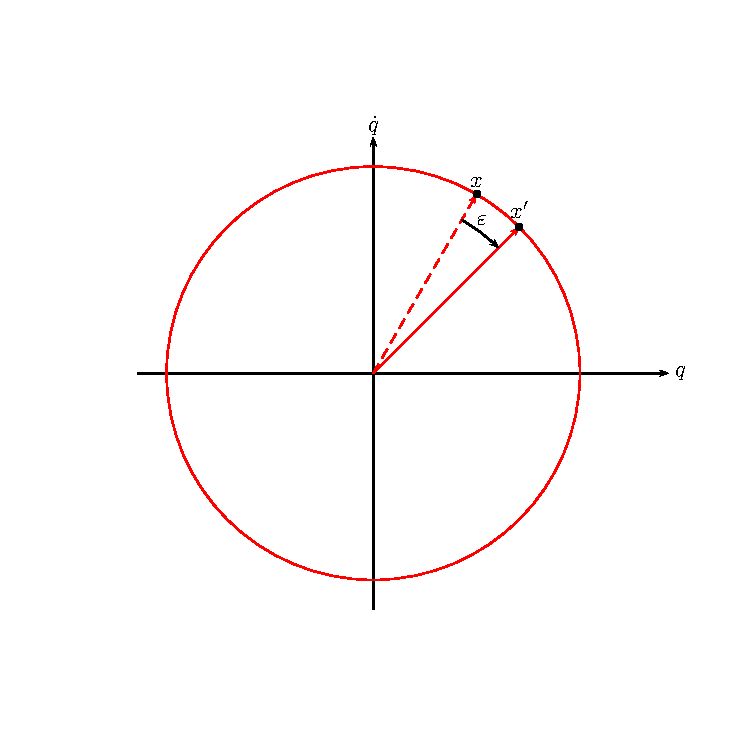
\includegraphics[width=0.5\textwidth]{TimeOffset}
    \caption{Offset Action}
    \label{fig:gtoff}
\end{center}
\end{figure}

For a dynamic system, time offset is symmetrical for all dynamic system.
At the first look, no control effort is needed.
In practise, time offset is achieved by applying time scaling twice, after applying time scaling $\ep$ for sometime, and then apply the inverse action(time scaling of $\frac{1}{\ep}$).


\subsection{Action Selection}
There are many actions available for motion adaptation.
In certain situations, there are many different ways to satisfy the motion constraints, causing the problem which action should be applied.
Different groups will result in different motion styles.
This idea is supported by lots of examples in Chapter~\ref{chap:walk}.
In practise, this is left for the animator to decide.
Usually, the symmetry of natural dynamic is preferred, for such actions are energy efficient.







\section{Example: Symmetry of the Bouncing Ball System}
\label{sec:symball}
Symmetry is a common property among many dynamic systems, even for the hybrid systems like the bouncing ball system of Equation~\ref{eq:bbeq}.
It is shown in this section that by utilizing the symmetry group, complex motions can be predicted in an computationally efficient way.

The bouncing ball system of~\ref{eq:bbeq} has a energy scaling symmetry.

The energy function of the bouncing ball system is  
\[
E=\mathrm{g}q+\frac{1}{2}m\qd^2
\]
If the energy is scaled up by $\ep^2$,  potential energy is scaled up by $\ep^2$.
 Because $V= \frac{1}{2}\mathrm{g}q$, and $\ep^2 V=\frac{1}{2}f(\ep)q$, thus:
\[
f(\ep)=\ep^2
\]
the energy scaling transformation is
\[
\gen(\state)=[\ep^2 q, \ep \qd]
\]

For the bouncing ball system, the energy of a system can be characterized by the initial dropping height.

Given the motion of a ball dropped at $5$ as shown in Figure~\ref{fig:bouncing5}, we set $\ep=\sqrt{2}$ and obtained the motion dropped from $10$ through the transformation as shown in Figure~\ref{fig:bouncing10}.
Figure  motion dropped from $10$ is shown in Figure~\ref{fig:bouncing10sim}.
\begin{figure}[!htbp]
  \begin{center}
      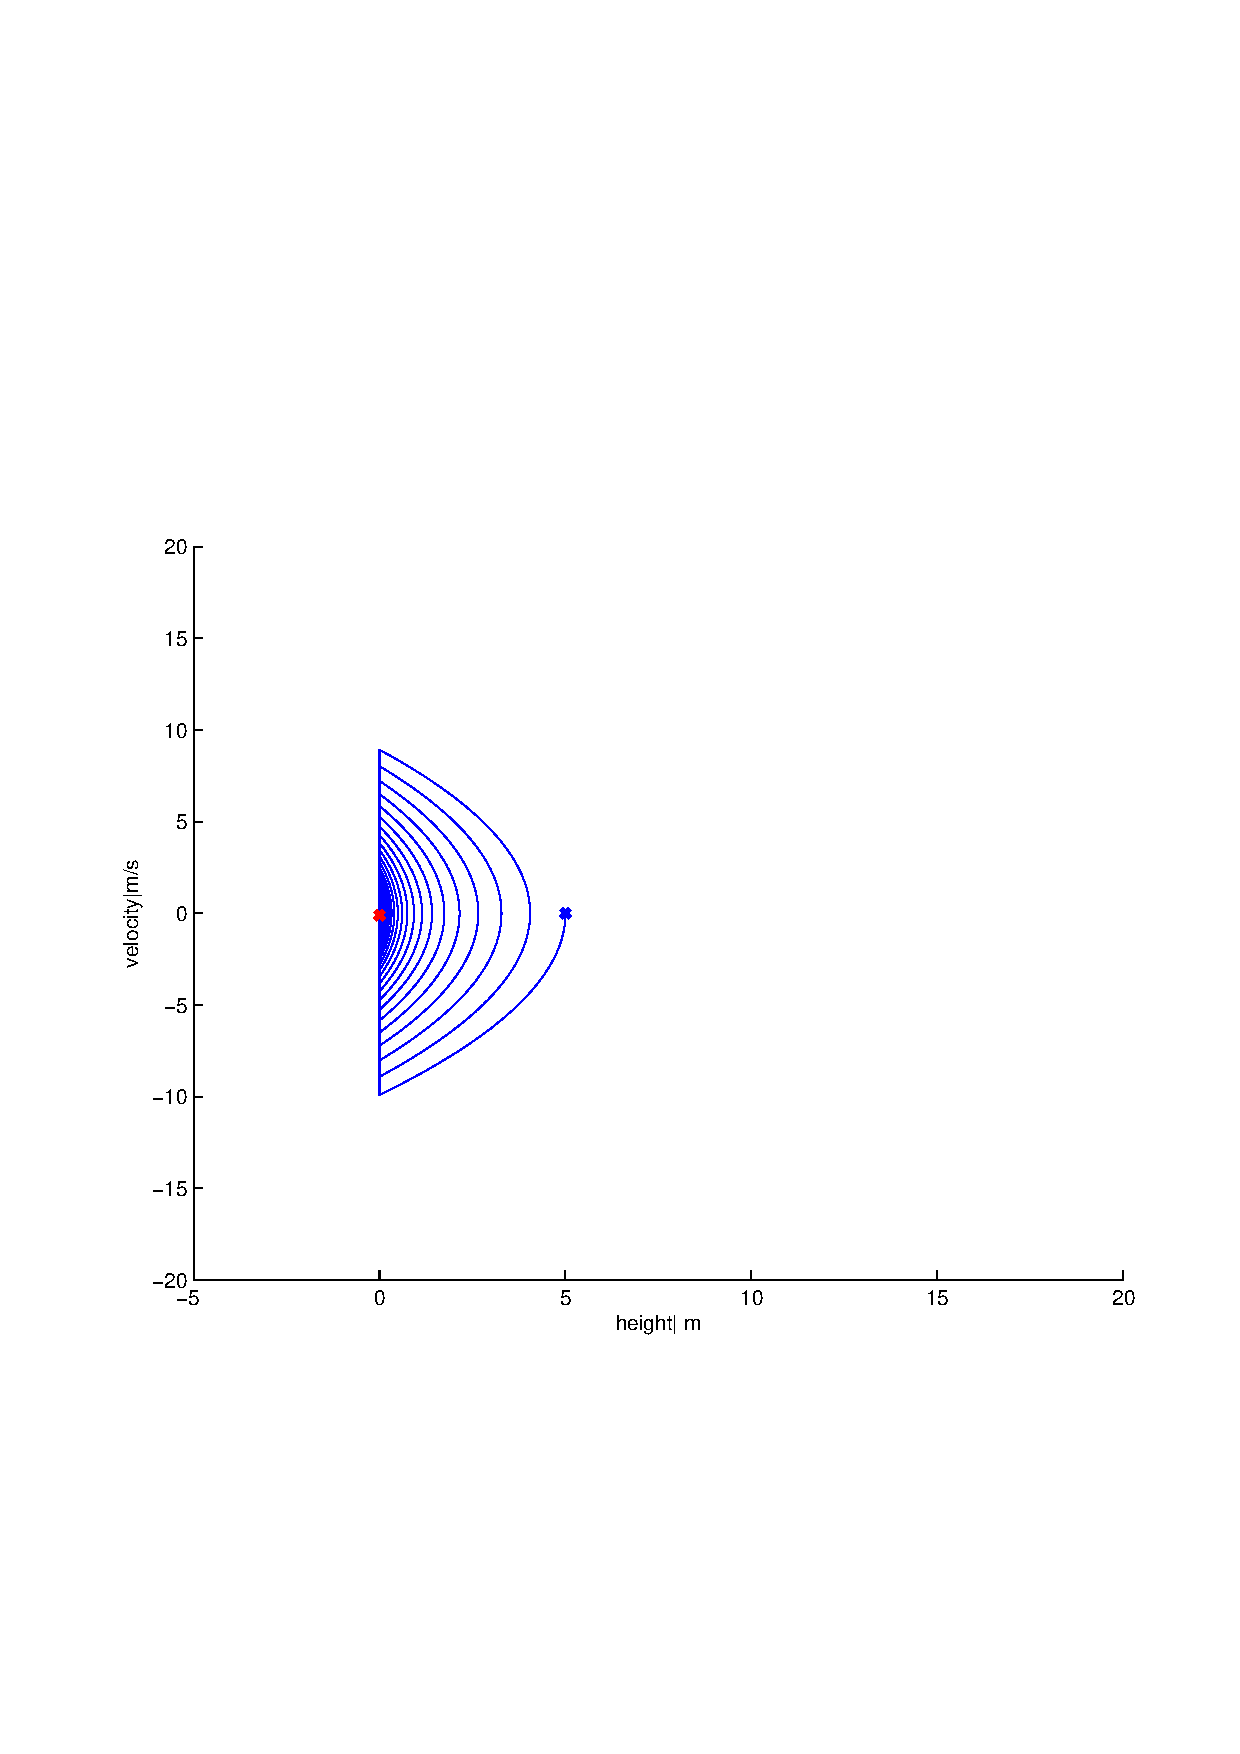
\includegraphics[width=0.5\textwidth]{BouncingBallPhasePlotuncontrolledDropAt5}
    \caption{Drop at 5}
    \label{fig:bouncing5}
\end{center}
\end{figure}


\begin{figure}[!htbp]
  \begin{center}
      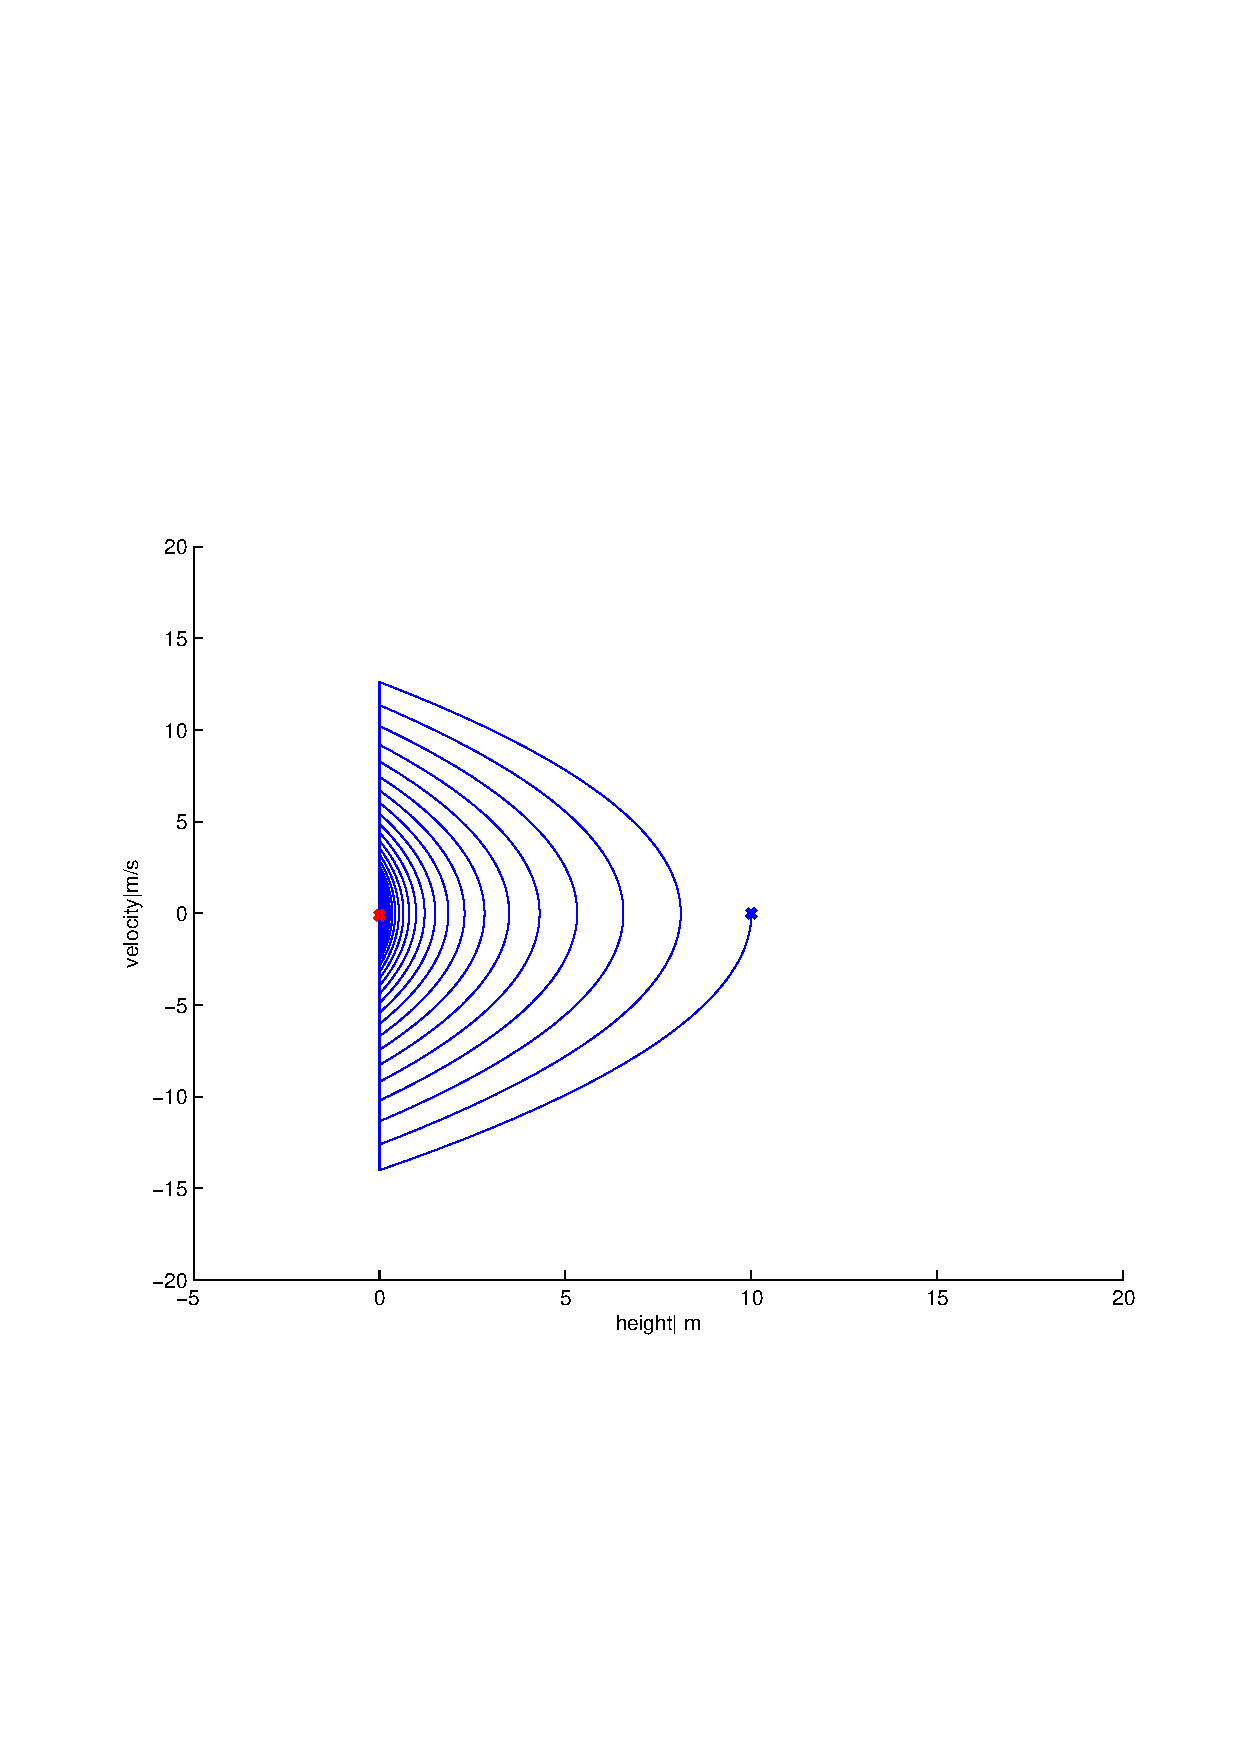
\includegraphics[width=0.5\textwidth]{BouncingBallPhasePlotuncontrolledDropAt10}
    \caption{Drop at 10 by transformation}
    \label{fig:bouncing10}
\end{center}
\end{figure}

\begin{figure}[!htbp]
  \begin{center}
      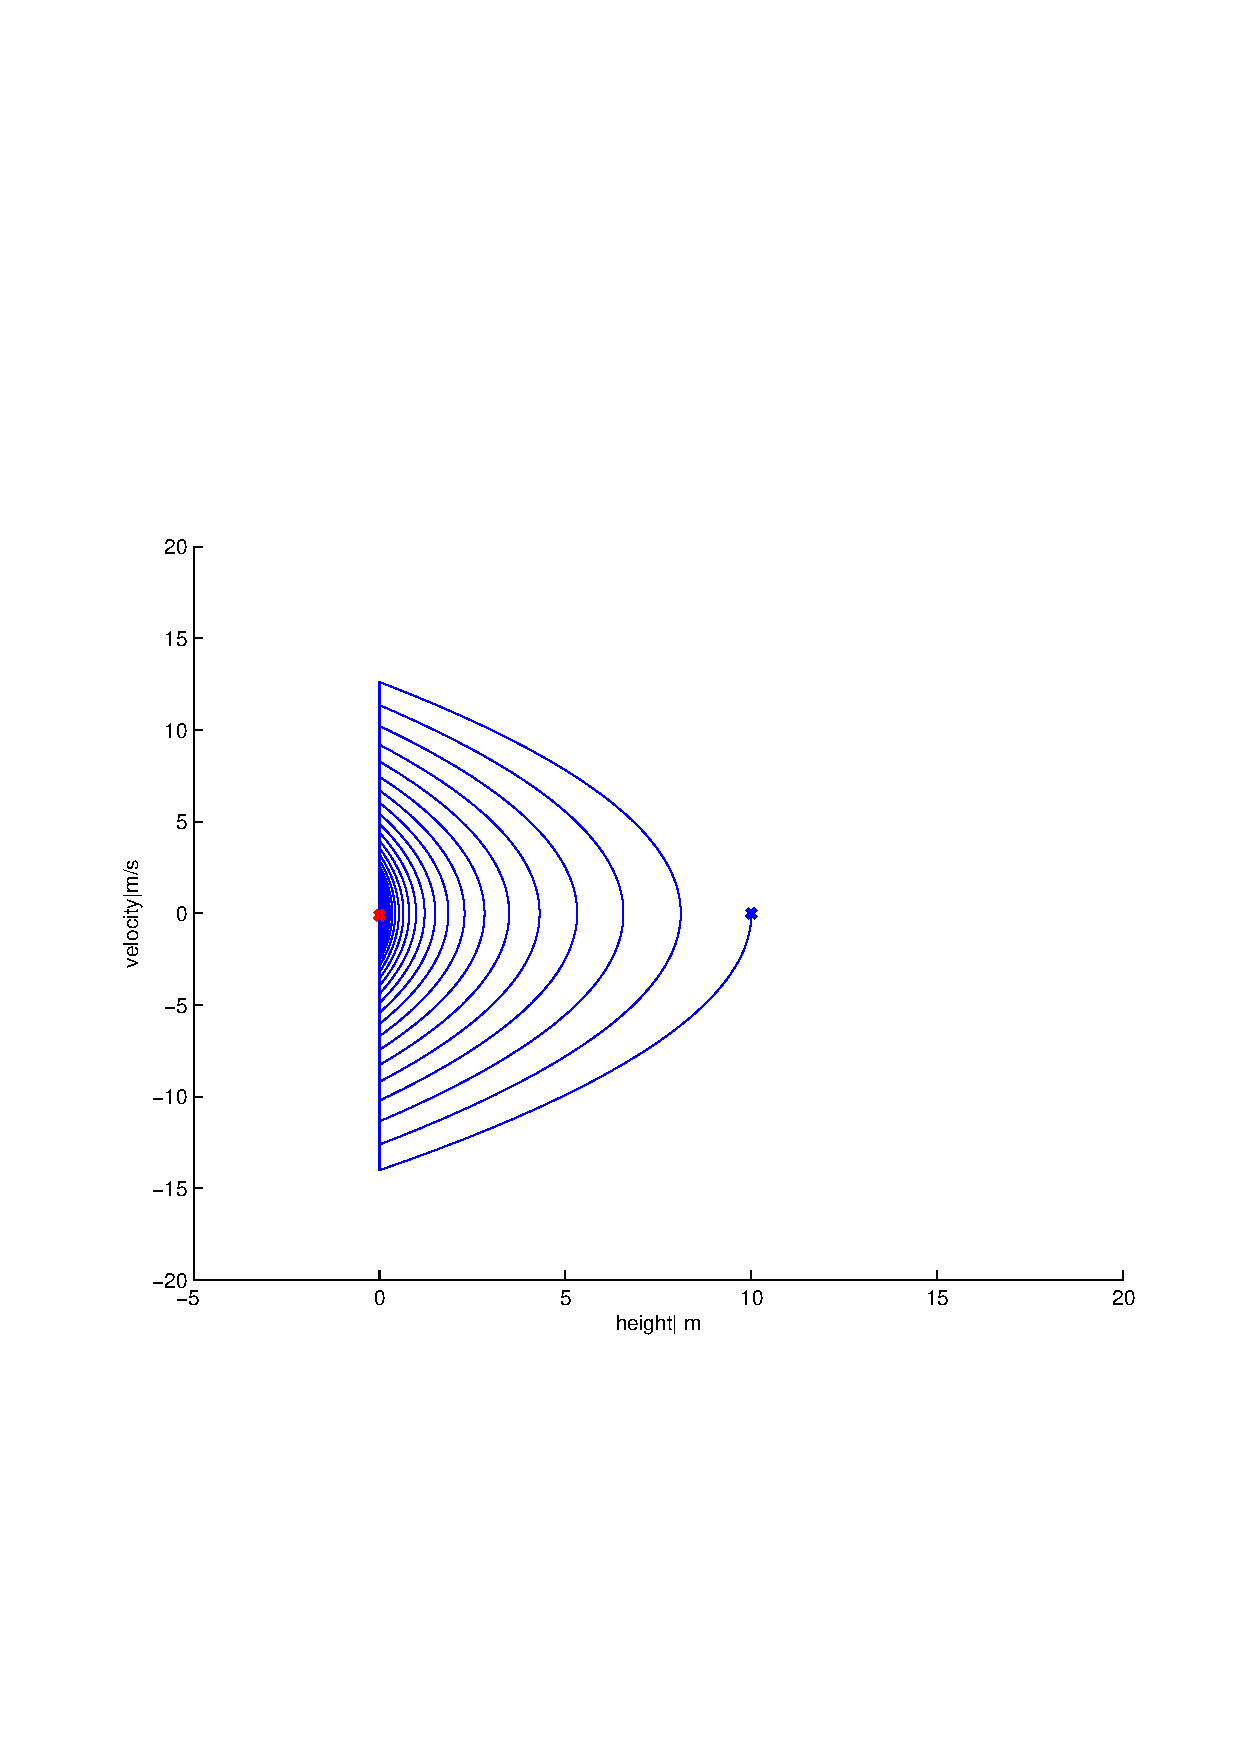
\includegraphics[width=0.5\textwidth]{BouncingBallPhasePlotuncontrolledDropAt10}
    \caption{The simulation result of dropped from 10}
    \label{fig:bouncing10sim}
\end{center}
\end{figure}




\chapter {MOTION SYNTHESIS FRAMEWORK}
\label{chap:msf}
\graphicspath{{CombineFramework/CombineFrameworkFigs/EPS/}{CombineFramework/CombineFrameworkFigs/}}

The ideas of Global Motor Invariant and Local Motor Invariant are dicussed separately in Chapter~\ref{chap:gi} and Chapter~\ref{chap:li}.
This chapter focuses on put these ideas into \cms application.
Two problems arised from combinations in application
\begin{itemize}
	\item Combine global and local motor invariant controller together.
	\item Combine different motion primitives together.
\end{itemize}

\section{Combined Motor Invariant Control}

\subsection{ Combine Motor Invariant Control}

Neural Oscillator will maintain the Global Motor Invariant and Controlled Symmetry will maintain the Local Motor Invariant.
Combining two controllers poses the question of violating the other invariant:
\begin{itemize}
\item From the Global Motor Invariant Perspective in Chapter~\ref{chap:gi},
when the controlled symmetry  is applied, it must not violate the topology. 
It is easy to prove that controlled symmetry maintains the topology.

\item From the Local Motor Invariant perspective in Chapter~\ref{chap:li}.
Controlled symmetry can only applied to mechanical system, the \cpg will not be effected by controlled symmetry.
When a group action is applied to the mechanical system, parameters of \cpg should be transformed accordingly to maintain the symmetry property.
This is called \emph{Adjoint Transformation}.
\end{itemize}


In application, to ajust the combined controller,
\cpg is applied first maintain the topology against the structural perturbation. 
Afterwards Symmetry Control is to meet application specific constraints.
This idea is illustrated in the following Figure ~\ref{fig:sysoverview}

\begin{figure}[!htbp]
  \begin{center}
      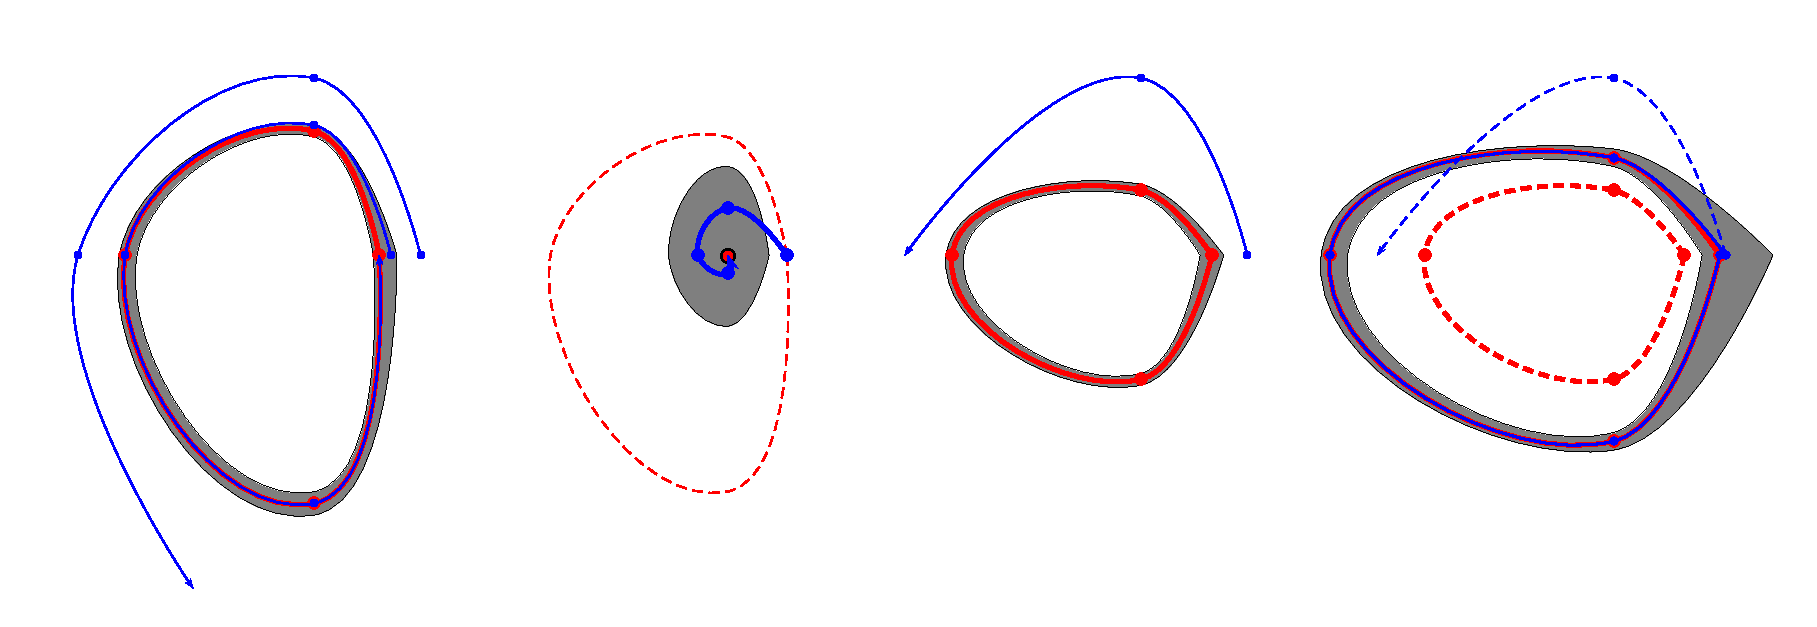
\includegraphics[width=0.7\textwidth]{LimitCircle}
    \caption{System Over View }
    \label{fig:sysoverview}
  \end{center}
\end{figure}


For the controlled symmetry's effect on topology, we have the following theorem:

\begin{mythe}
Transformation of Control Symmetry is Topological Conjugation
\end{mythe}
\begin{proof}
This theorem is easy to prove by checking properties of group.
\end{proof}

\subsection{Adjoint Transformation of \cpg}
Adjoint Transformation modify the parameters of neural oscillator to maintain the symmetry.

Coupled with neural oscillator, the dynamic system 
\[
\dot{\state}=F(\state)
\]
becomes a system 
\begin{equation}
\label{eq:gc}
\dot{\state}=F(\state)+D\uout
\end{equation}


When the symmetry group action $g$ is applied, the Equations~\ref{{eq:gc}} are transformed into
\begin{equation}
\label{eq:cc}
Tg(\dot{\state})=F(g(\state))+DTg(\uout)
\end{equation}




If symmetry is preserved, the Equation~\ref{eq:con} and Equation~\ref{eq:cc} should be equivalent.
\begin{equation}
\label{eq:con}
\dot{\state}=F(\state)+\ulocal+D\tilde{\uout}
\end{equation}
$\tilde{\uout}$ is the output of neural ssytem after adjoint transformation.
As show in equation~\ref{eq:simplematsuta},$\uout$ is a function of $\uin$.
Control effort can not be directly on neural oscillator, transformation of $\uout$ is achieved by modifying the system's parameters.



\begin{myprop}
By modifying parameter $\tau_{1,2}$
\[
\tau_{1,2} \mapsto \ep \tau_{1,2}
\]
is equivalent to time scaling the neural oscillator by parameter $\ep$.
\end{myprop}
\begin{proof}
By subsitute $\tilde{\tau}_{1,2}=\ep \tau_{1,2}$, and $\tilde{t}=\frac{t}{\ep}$, the Equation~\ref{eq:matsuta} will remain the same.
\end{proof}

Based on the propostion above, a scheme of adjoint transformation to modify the parameters $\tau_{1,2}$,$\hin$,$\hout$ for maintain the symmetry of the  coupled system.
The input and output of neural are chosen to maintain the shape.
\begin{enumerate}
\item Modify $\tau$ by the time scaling parameter $\tau \mapsto \ep \tau$.
\item Input variable $w$ and input efficient $\hin$ are modified to make sure the input function statisfy the time scaling symmetry $\uin(t) \mapsto \uin(\frac{t}{\ep})$
\item  Parameters of $\hout$ are modified according to $D$, or how the mechanical system is drived.
If $\uout$ drive the position variable $q$ then, $\hout$ should multiplied by the position scale factor. 
If $\uout$ drive the velocity,$\hout$ is multiplied by the speed scale factor.
If the $hout$ is force and acting on the acceleration $\ddot{q}$, then $\hout$ is multiplied by the acceleration scale facotr.
\end{enumerate}


According this adjoint transformation strategy, we can get the following thereom
\begin{mythe}
For a transformation group $G$, if the parameters of the neural oscillator are modified according to adjoint transformation.
 Combined system preserving symmetry $I^G$.
\end{mythe}
For prove, readers can check the symmetry by substitute transformed variables into the original system to check the symmetry.

Thus both the Local Motor Invariant and Global Motor Invariant are maintained
For the specific symmetry types proposed in Chapter~\ref{chap:li},several example of adjoint symmetry are provideds


\subsubsection*{ Offset Symmetry.}
For offset symmetry:
\[
(t,q,\qd) \mapsto (t,q+\ep,\qd)
\]
there is no time scaling effects.
To maintain the shape of $\uin$ and $\uout$,  $\uin$ and $\uout$ are functions in invariant space.
For example, the input of the neural oscillator are chosen to be the angle difference between the joints or velocity.



\subsubsection*{Time Scaling}
For time scaling:
\[
(t,q,\qd) \mapsto (\frac{t}{\ep},q,\ep \qd)
\]
Adjoint Transformation
$\tau \mapsto \ep \tau $.
if the output$\uout$ is applied as force, then $\hout \mapsto \ep^2 \hout$

\subsubsection*{ Energy Scaling}
Energy Scaling is combined action of time scaling and posture scaling:
\[
(t,q,\qd ) \mapsto ( \frac{f(\ep)}{\ep}t ,f(\ep)q,\ep\qd)
\]
the time scalling factor is $\frac{\ep}{f(\ep)}$, 

The parameters $\tau_{1,2}$ are transformed
\[
\tau_{1,2} \mapsto \frac{\ep}{f(\ep)} \tau_{1,2}
\]
To maintain the time scaling symmetry of $\uin$, if the input valuable is $\qd$, 
then 
\[
\hin \mapsto \ep \hin
\]
if the output drive the velocity, then the output is $\hout$
\[
\hout \mapsto \ep \hout
\]




\subsection{Example: Height Control of Bouncing Ball}

Bouncing Ball has energy scaling symmetry; a limit cycle emerged when coupling with neural oscillator.
By combining both motor invariant controllers, the limit cycle can be controlled.
Then the bouncing height can be controlled.

\subsubsection*{Adjoint Transformation}
Suppose the coupled system is bouncing at height of $5$
For the energy scaling:
\[
(t,q,\qd ) \mapsto ( \ep t ,\ep^2 q,\ep \qd)
\]

According to the system transformation
the time scaling factor is $\ep$, we have:
\[
\tau_{1,2} \mapsto \alpha \tau_{1,2}
\]

The input to the neural oscillator is $\qd$,
\[
\hin \mapsto \frac{\hin}{\ep}
\]
 
Neural Oscillator drives the position of the paddle, the output $\uout$ needs to be scaled by the position scale value.
For $q \mapsto \ep^2q$, we have
\[
 \hout \mapsto \ep^2 \hout
\]

When $\ep^2=3$, then the ball will bounce at height of $15$, and it maintain its topological structure, which is a limit cycle.
as shown in Figure ~\ref{fig:energy3}. 
By this method, arbitrary bouncing height can be controlled.


\begin{figure}[!htbp]
  \begin{center}
   	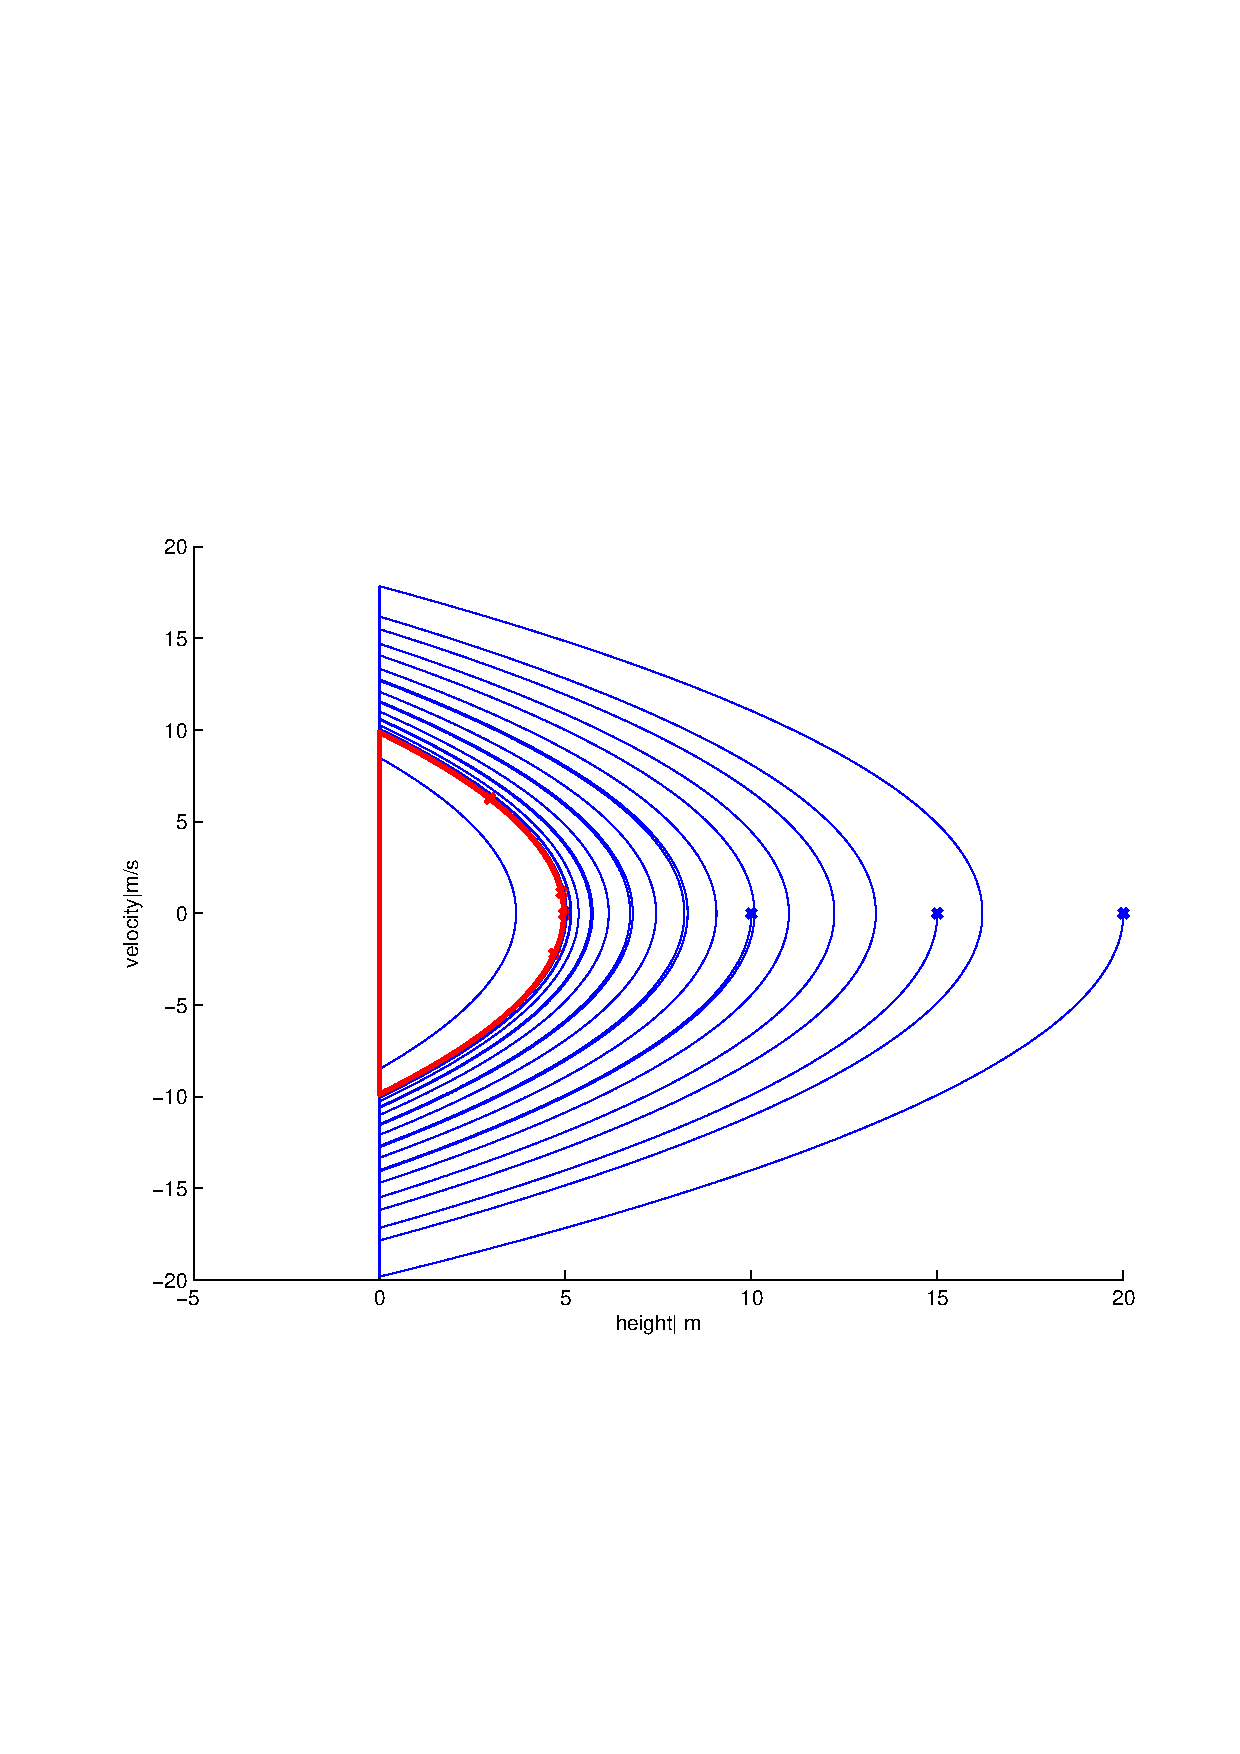
\includegraphics[width=0.7\textwidth]{BouncingBallPhasePlotAction1}
    \caption{Energy Scalling}
    \label{fig:energy1}
  \end{center}
\end{figure} 


\begin{figure}[!htbp]
  \begin{center}
	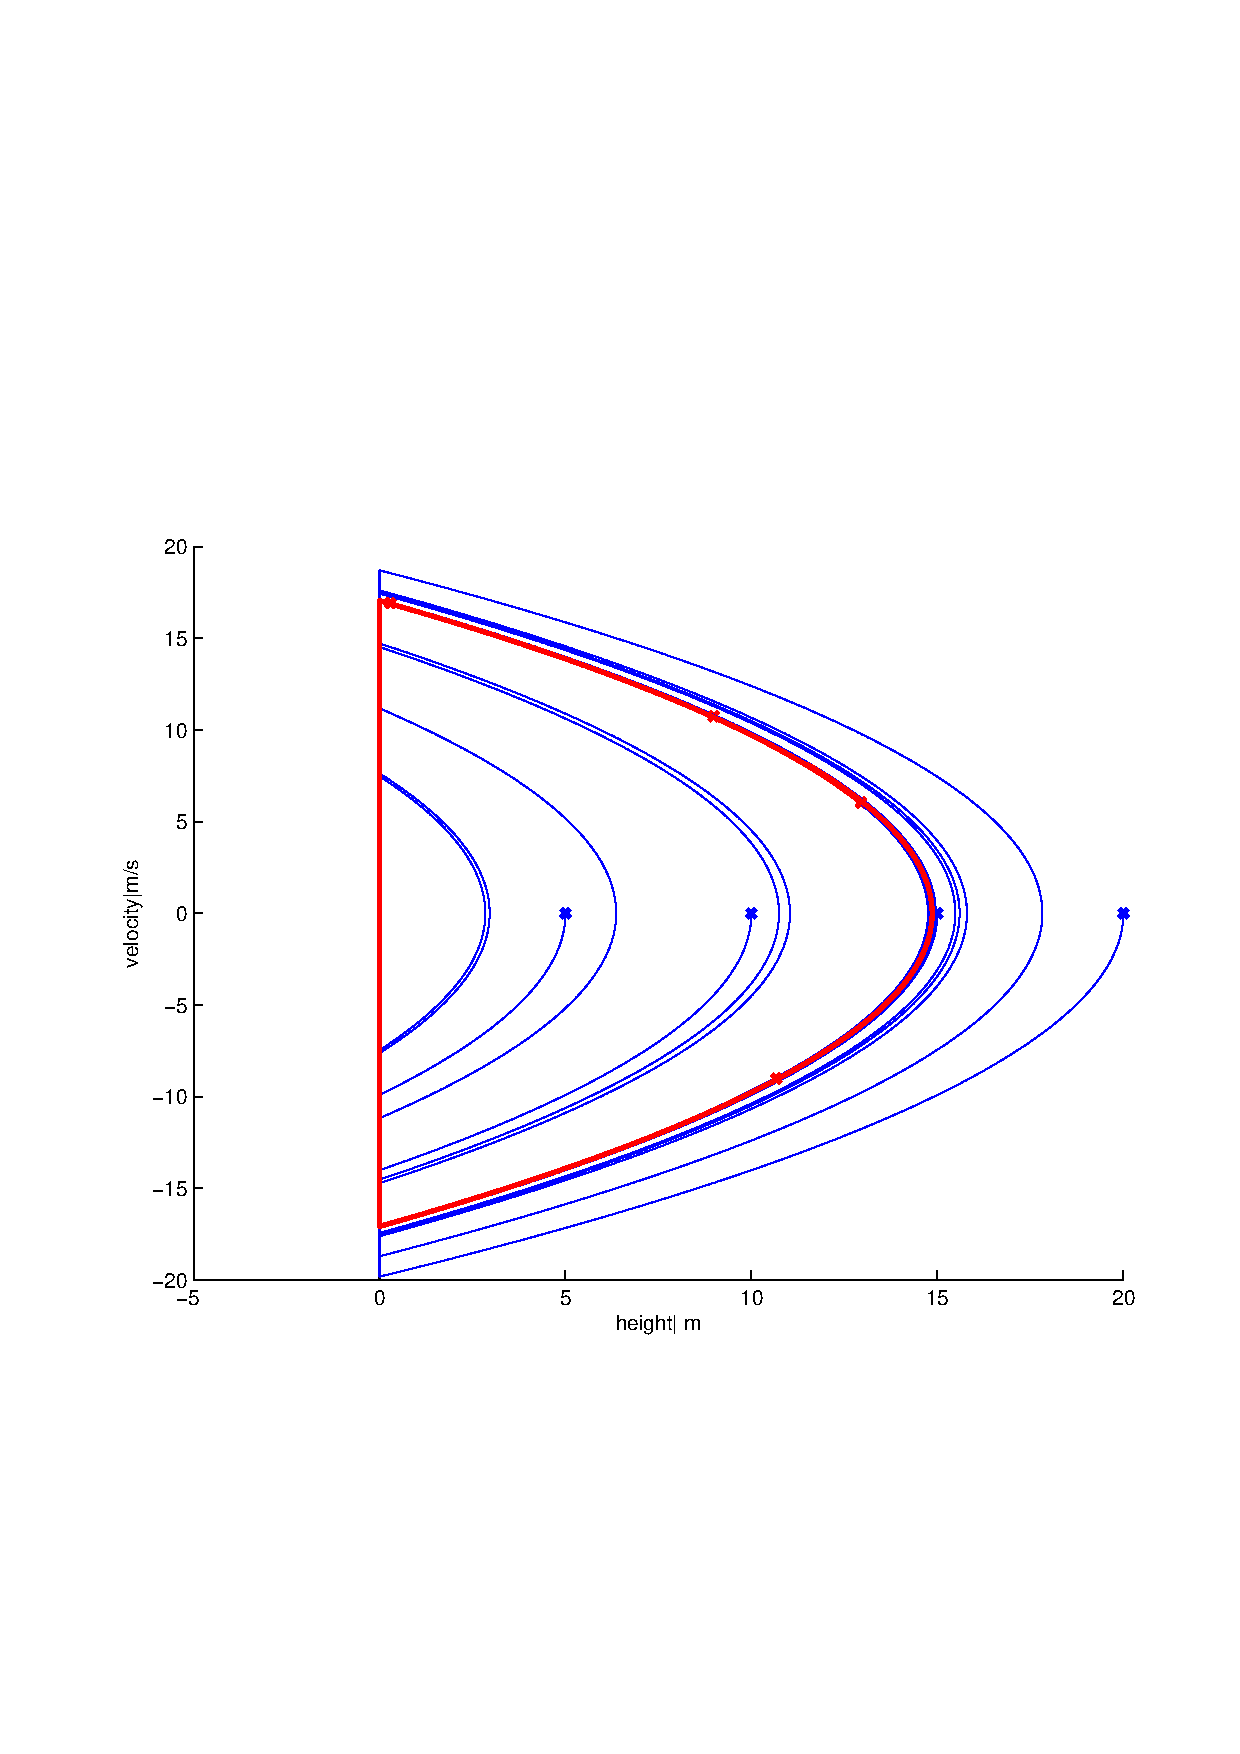
\includegraphics[width=0.7\textwidth]{BouncingBallPhasePlotAction3}
    \caption{Energy Scaling}
    \label{fig:energy3}
  \end{center}
\end{figure}

\section{Combine Motion Primitives}

\subsection{Dynamic Motion Graph}
The topological structure of the natural mechanical syste form a graph structure:
Each motion primitive is represented as a node, and two nodes are conneced if they are near each other on the phase plot.
This graph is the \emph{Dynamic Motion Graph}.

The idea is very similar to the \emph{Motion Graph}\citep{kovar2008motion}, the difference is in the  Motion Graph are handed crafted.
While in our research,  the dynamic motion graph is fixed, from any motion primitive, the motion primitive a character can changed to is limited.

\begin{figure}[!htbp]
  \begin{center}
	\includegraphics[width=0.7\textwidth]{MotionPrimitiveGraph}
    \caption{Phase Plot of Motion Primitives}
    \label{fig:manyprimitives}
  \end{center}
\end{figure}


\begin{figure}[!htbp]
  \begin{center}
      \includegraphics[width=0.7\textwidth]{motiongraphtopology}
    \caption{Phase Plot of Motion Primitives}
    \label{fig:manyprimitives}
  \end{center}
\end{figure}


\subsection{Dynamic Motion Primitives Transition}
From  the dynamic perspective, motion primitive transition means move the current $\state$ from the basin of attraction of one attractor into another, as shown in Figure~\ref{fig:motion-transition}.
Without any effort, the transition will not happen automatically, for the two basic of attractions do not overlap.



\begin{figure}[!htbp]
  \begin{center}
      \includegraphics[width=0.7\textwidth]{MotionPrimitiveTransition}
    \caption{Motion Primitive Transition}
    \label{fig:motion-transition}
  \end{center}
\end{figure}


Based on the two methods for motor invariant control, two methods are proposed for motion primitive transition.
\begin{itemize}
\HiItem{Entrainment Overlap}
Empirically,when \cpg is applied for one motor primitive $\mathcal{A}$, the basin of attraction $\mathcal{Bo}(\mathcal{A})$ is enlarged.
If \cpg are applied for two motion primtives $\mathcal{A,A'}$ seperately, the enlarged basin of attractions $\mathcal{Bo}(\mathcal{A})$,
%$\omicron$
$\mathcal{Bo}(\mathcal{A'})$ will overlap.
\[
O =
\mathcal{Bo}(\mathcal{A}) 
\bigcap \mathcal{Bo}(\mathcal{A'}) 
\neq \varnothing
\]
 
If  state $\state$ lies in the $O$, by switch the \cpg controller, motion primitive is also switched, as shown in Figure~\ref{fig:motion-overlay}.


\begin{figure}[!htbp]
  \begin{center}
      \includegraphics[width=0.7\textwidth]{OverLayTransition}
    \caption{OverLay Transition}
    \label{fig:motion-overlay}
  \end{center}
\end{figure}


\HiItem{Transform Method}
Controlled Symmetry can also apply for motion primitive transition.
For a system at $\state$,  The phase portrait can be transformed to move the basin of attraction,as shown in Figure~\ref{fig:transform-offset}.


\begin{figure}[!htbp]
  \begin{center}
      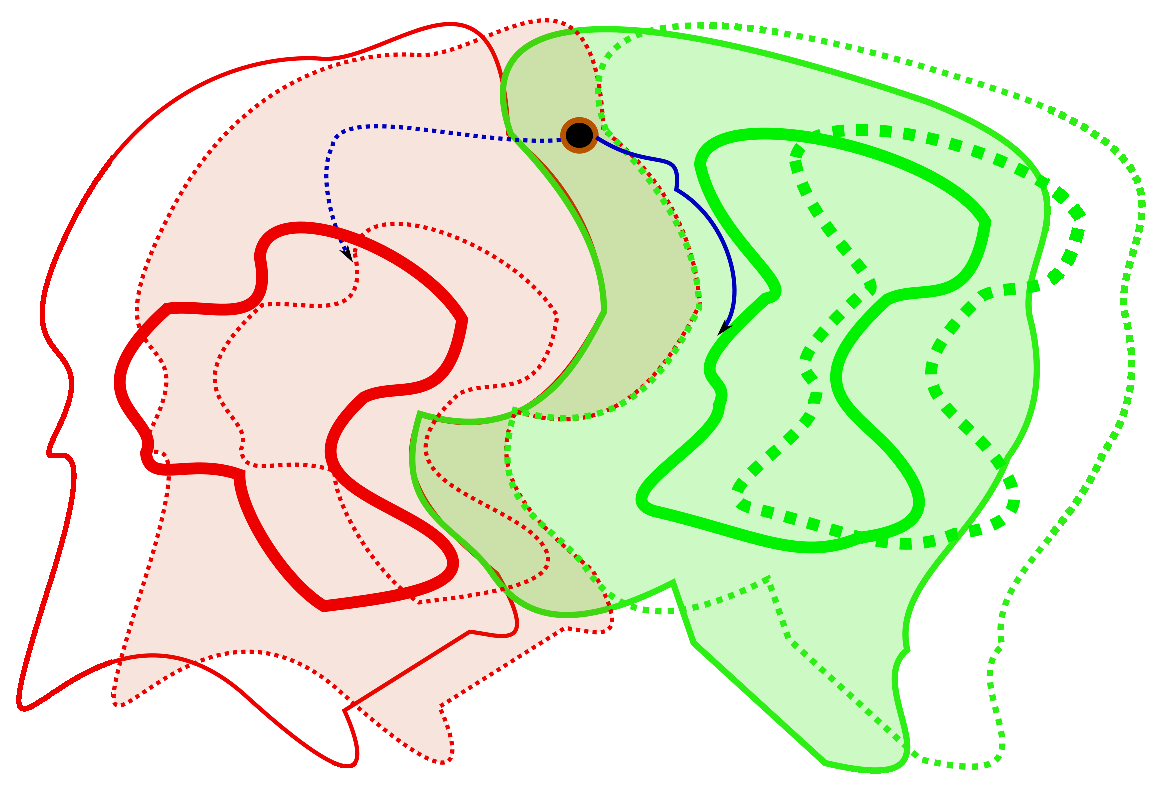
\includegraphics[width=0.7\textwidth]{OffsetTransition}
    \caption{Offset Transiton}
    \label{fig:transform-offset}
  \end{center}
\end{figure}
\end{itemize}




Both the method can result in physically realistic motion transition, but requires $\state$ lies at specific reason.
In motor invariant theory, the current state $\state$ is not directly controlled.
The measure is make the overlap region $O$ cover part of both attractors$\mathcal{A}$,$\mathcal{A'}$.

The state $\state$ is going to converge to the attractor $\mathcal{A}$.
The overlap region cover both attractors $\mathcal{A}$, $\mathcal{A'}$,bidirectional transitions are possible when motions are near stable state.

When Controlled Symmetry is applied, both motion primitives are transformed, there is relationship between the two transformations; \emph{transformation connection}, as shown in Figure~\ref{fig:Combine}

\begin{figure}[!htbp]
  \begin{center}
      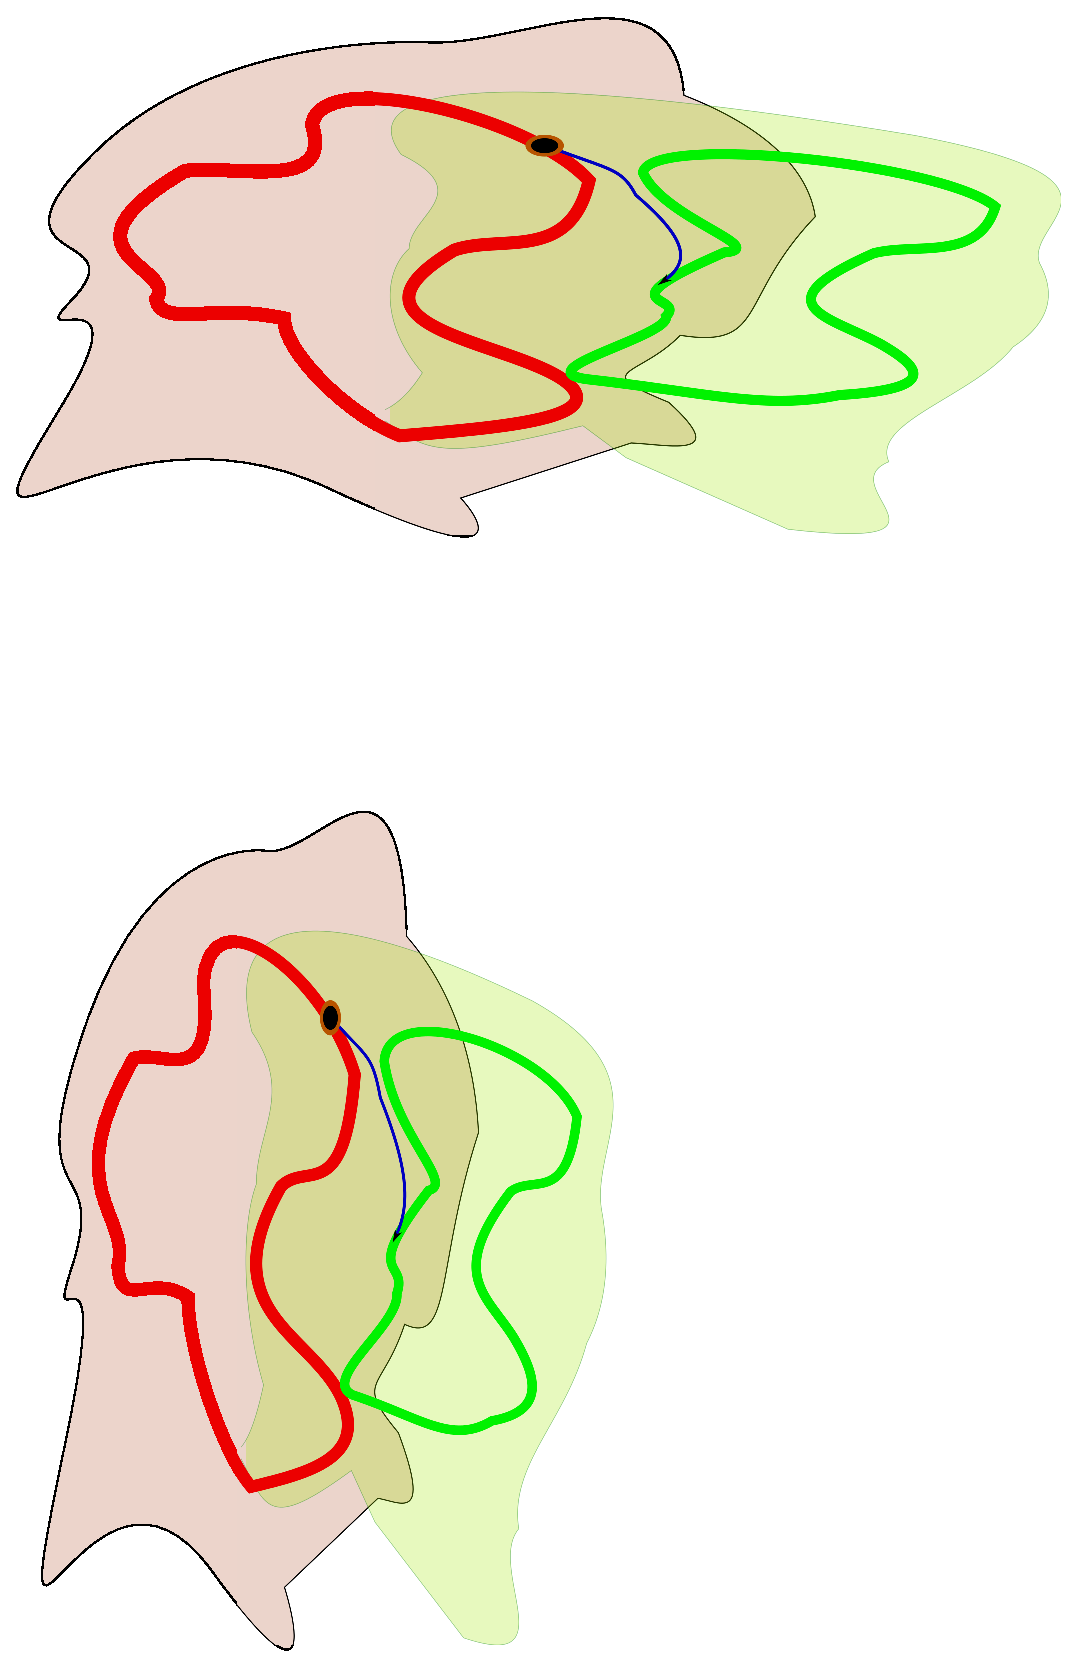
\includegraphics[width=0.7\textwidth]{ConbineMethod}
    \caption{Comined Method}
    \label{fig:Combine}
  \end{center}
\end{figure}

\section{Motion Synthesis Framework}
While this procedure may appear mathematically complex, applying this method for motion synthesis is straightforward. 
You will need:
\begin{enumerate}
\item a mechanical oscillator $F(\x)$ which best describes the body and environment
\item a neural oscillator (for example, the Matsuoka oscillator in Equation~\ref{eq:matsuta}) and associated parameters,that form a limit cycle

\item an action $g \in G$ which adapts the problem to the current environment (we present three possible operators in Section~\ref{sec:control_symmetry}). the adjoint system transformation  is applied to the neural oscillator parameters.

\item an integrator to solve the system (we use the fourth order Runge--Kutta method provided in the {MATLAB} function \emph{ode45}).
\end{enumerate}
In the following chapters, this method is applied to generationg adaptive motions.




\chapter{MOTION PRIMITIVE TWEAKING:BIPEDAL WALKING}
\label{chap:walk}
\graphicspath{{BipedWalk/BipedWalkFigs/EPS/}{BipedWalk/BipedWalkFigs/}}


The examples of bouncing ball and mass spring systems explain the idea well.
However, they are are too simple for \cms\ applications.
This chapter focus on more controlling more complex mechanical system which have great application value.  
Details are given about how to adapt a motion primitive for  environmental and application specific constraints.
Combination and transitions of motion primitives are discussed in the next chapter.


The motion primitive under study in this chapter is \emph{bipedal walking}, which is a topic of great application value for both the graphic and robotic engineering.
Although many methods have been applied to the bipedal walking in the past decades, human bipedal walking ability still has not been achieved. 
The early belief is that bipedal walking is unstable in nature, and many control methods are developed based on trajectory tracking principle.
The turning point is the discovery of the passive dynamic walking machine, which shows that under specific conditions, walking can happen naturally without the need of any control effort.
This makes us believe that the walking ability is inborn, and most control problems have already been solved by the mechanical structure.

From the perspective of \moit, bipedal walking is  a motion primitive.
In this chapter, the passive walking gait is treated as the motion template.
Neural Oscillator and Symmetry Control efforts are applied to tweaking the template while maintaining the global and local motor invariants.
This method is capable of generating adaptive and stable gaits in real-time.
This process may provide a clear example of application of the \moit\ idea.




\section{the Bipedal Walking Primitives}


Bipedal means ``two feet'' (Here, ``bipedal'' is from the Latin bi for "two" and ped for "foot"). 
With two legs, animals can walk, run and jump.
Relatively few modern animals use two legs for normal locomotion. 
For human, bipedalism evolved well before the large human brain or the development of stone tools.
So human are capable of bipedal walking long before the ages of intelligence.





The walking of human is characterized by an ``inverted pendulum'' movement in which the body vaults over a stiff leg with each step.
During walking, hips rotates about the axis of the spine, to increase stride length, and it also rotates about the horizontal axis to improve balance during stance.


In \moit, walking is treated as an independent motion pattern.
To illustrate the idea without unnecessary complexity, the walking dynamics is simplified.


\begin{figure}[!htbp]
  \begin{center}
    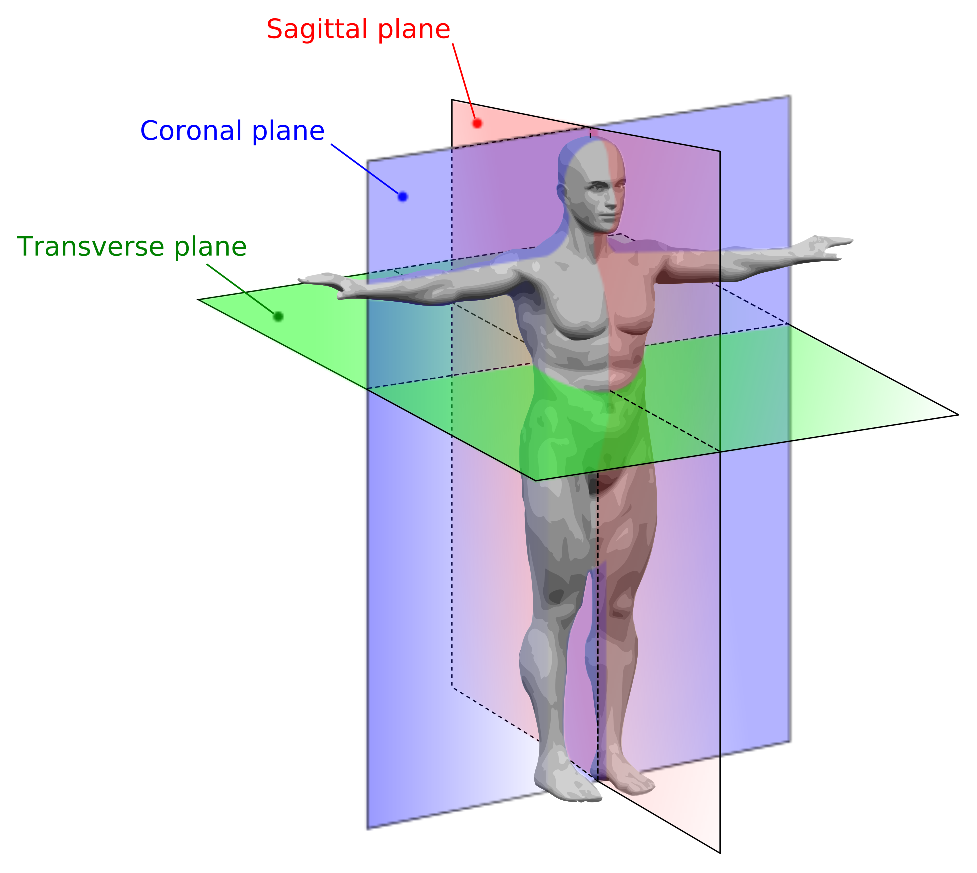
\includegraphics[width=0.5\textwidth]{spahittalPlae}
    \caption{Sagittal Plane}
    \label{fig:sgplane}
\end{center}
\end{figure}

As shown in Figure~\ref{fig:sgplane}, motion is projected into three spaces:the sagittal plane, coronal plane and transverse plane.
For bipedal walking,
 yaw and roll motion are relatively small and usually treated as secondary motion or totally neglected,  the main motion happens in the \emph{sagittal plane}.




Due to the above reason, this chapter focuses on the motions in sagittal plane, and  the motions of other \dof s in coronal plane and transverse plane are discussed in Chapter~\ref{chap:highdor}.
Such a simplification will not change the basic motion characteristics and adaptation tendency.
Since more {\dof}s will make the ``symmetry'' not so perfect and may cause confusions in explaining the idea, the discussions about more {\dof}s are delayed.



\subsection*{Dynamics}

The simplified walking model is shown in Figure~\ref{fig:passivekneewalker}.

\begin{figure}[!htbp]
  \begin{center}
    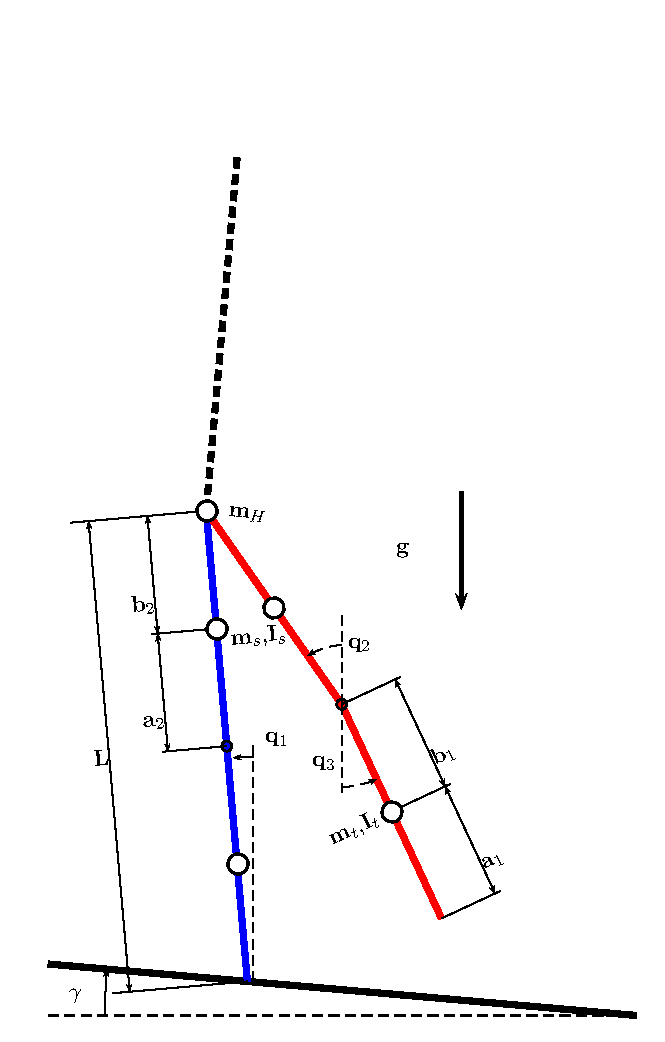
\includegraphics[height=0.4\textheight]{PWI}
    \caption{A Passive Walking Model with Knee}
    \label{fig:passivekneewalker}
  \end{center}
\end{figure}
The walking model of Figure~\ref{fig:passivekneewalker} is based on rigid body dynamics.
The supporting leg is kept straight.
In the figure, $L$ is the length of the leg, $q_1$ is the angle of the supporting leg,
$m_t$ and $m_s$ are the mass of the shank and thigh,
$q_2$ and $q_3$ are the corresponding angles of the swinging shank and thigh,
$b_1,a_1$ and $b_2,a_2$ describe the relative position of gravity center,
$m_h$ represents sum mass of the body and hip .






Like the bouncing ball system, this dynamic system is hybrid\citep{ames2006categorical} and includes both continuous and discrete dynamics.
Passive walking with knees includes four phases\citep{Chen2007}.
\begin{itemize}
\HiItem{Free Swing Phase}
The support leg (the blue one) is kept straight.
During this phase, the knee of the swing leg is bended, and the thigh and shank swing freely.
\HiItem{Knee Strike Phase}
The knee joint of the swing leg has a limit.
When the knee angle reaches the limit, a collision happens.
After the collision, the swing leg is kept straight.
\HiItem{Knee Lock Swing Phase}
During this swing phase, both the swing and support leg are kept straight.
\HiItem{Heel Strike Phase}
When the heel of the swing leg hits the ground, a collision happens.
After that the swing and support legs are switched.
\end{itemize}

Figure~\ref{fig:fwalkingphase} shows the gaits of four phases.
\begin{figure}[!htbp]
  \begin{center}
      \includegraphics[width=0.7\textwidth]{Fourphase}
    \caption{The four phases in Walking}
    \label{fig:fwalkingphase}
\end{center}
\end{figure}





\begin{itemize}
\HiItem{Flying Phases}
Both the free and locked knee swing phases are described by the continuous dynamics.
Both equations are in the form of Equation~\ref{eq:flyequationpwi}.
\begin{equation}
\label{eq:flyequationpwi}
M(\mathbf{q}) \ddot{\mathbf{q}} + C(\mathbf{q,\qd})\dot{\mathbf{q}} + N(\mathbf{q}) = 0
\end{equation}
where $q=[q_1,q_2,q_3]$,$\qd=[\dot{q_1},\dot{q_2},\dot{q_3}]$,$M$ is the initial mass matrix,  and $C$ and $N$ are the centrifugal force matrix and gravity respectively. 
For Knee Free Phase,  $M$ and $C$ are $3$ by $3$ matrix, and $N$ is $3$ by $1$ vector.
for Knee Lock Phase, $M$ and $C$ are $2$ by $2$ matrix, and $N$ is $2$ by $1$ vector.
Putting them into the standard form, and define $\state=[q,\qd]$, Equation~\ref{eq:flyequationpwi} is transformed into Equation~\ref{eq:stateformpw}
Then the function is in the form.
\begin{equation}
\label{eq:stateformpw}
\dot{\state}=
-\left[ 
\begin{array}{cc}
\mathbf{1} &0\\
0 &M 
\end{array}
\right]^{-1}
\left[ 
\begin{array}{cc}
0 &\mathbf{1}\\
0 &C 
\end{array}
\right]\state
-\left[ 
\begin{array}{c}
\mathbf{0}\\
 N 
\end{array}
\right]
\end{equation}

\HiItem{The Strike Phases}
The knee strike and heel strike phases are modelled based on discrete dynamics.
Collision equations are developed based on momentum preserving principle.
Both collision equations are in the form of Equation~\ref{eq:collidequ}.
\begin{equation}
\label{eq:collidequ}
J^{+}\dot{\mathbf{q}}^{+} = J^{-}\dot{\mathbf{q}}^{-}
\end{equation}

where $J$ is the matrix of angular momentum inertia, and the superscripts~$+,-$ represent those after and before collision respectively.
For Knees Strike,$J^-$ is a $3$ by $2$ matrix, $J^+$ is $2$ by $2$ matrix;
For Heel Strike, both $J^{+,-}$ are $2$ by $2$ matrix.
\end{itemize}
Dynamic equations are developed based on Lagrange Mechanics~\citep{Goldstein2002}.
For details of calculating the dynamic equation, please refer to \citep{Chen2007}
For the components of each matrix, please refer to the appendix.


\begin{figure}[!htbp]
  \begin{center}
    \includegraphics[width=0.7\textwidth]{walk_cycle_index}
    \caption{Four Phases Marked on a Walking Cycle}
    \label{fig:phasesmaker}
\end{center}
\end{figure}

With special initial conditions, the passive walker can walk down the slope with a stable gait.
On the phase plot,  a limit cycle emerges. 
Figure ~\ref{fig:phasesmaker} shows the phase plot of one thigh for a stable walking cycle.
where the events that separate the four phases are marked. 

In theory, the generalized coordinates for walking have $4$ degrees of freedom, with angle for shank and thigh for each leg.
Since the state space is $8$ dimension, it is not possible to draw the phase portrait on a $2$ dimension picture.
However, considering that motions of the two legs are almost the same, it is enough to show one leg motion, the state space is reduced to $4$ dimensions.
In the further analysis, we will indicate that the knee motion is not very important since the motion of the thigh captures the most valuable motion.
Thus we only draw the phase plot of the thigh of one leg.
Figure ~\ref{fig:phasesmaker} only shows the motion of the right leg.
The green plot shows the stance phase. 
During this phase, the right leg is supporting the body.
The blue parts show the swing phase.
During this phase,  the right leg is swinging and the left leg is supporting the body.
The yellow lines mark the $4$ collision events during walking.
Note that during the collision, the walking dynamic is discontinuous, and the speed of walking is changed suddenly without changing the position.
This means the yellow segments are not on the limit cycle. 
If the walker starts from the state in the middle of the yellow segment, it will fall.











\section{Global Motor Control and Adaptive Gaits}
The Passive Dynamic Walker exhibits a natural looking gait.
However, the walking motion is not stable.
In \moit, the repetitive walking motion suggests that the natural walking dynamic forms a limit cycle.
It seems that humans utilize the limit cycle for walking,  results in high energy efficiency.

To overcome the fragile stability, \cpg\ is applied with the hope to make the walking more stable through entrainment.
Experiments have shown that stability is enhanced and different perturbations result in varied and natural looking responsive motions.




\subsection{Entrainment}
For walking, only one neural oscillator is applied to maintain the stability of limit cycle.
The output of neural oscillator works as torque applied to hip angel (angle between the two thighs).
The dynamics are shown in Equation~\ref{eq:neuralwalk}
\begin{equation}
\label{eq:neuralwalk}
M(\mathbf{q}) \ddot{\mathbf{q}} + C(\mathbf{q,\qd})\dot{\mathbf{q}} + N(\mathbf{q}) = D\uout
\end{equation}
For the knee lock phase, $D=[1,-1]^T$.
For the knee free phase, $D=[1,-1,0]^T$.
This means the neural oscillator controls the thigh, and the knee is left to swing freely.

The input signal is the hip angle.
We have 
\[
	\uin=\hin(q_1-q_2)
\]





\begin{figure}[!htbp]
  \begin{center}
    \includegraphics[width=0.5\textwidth]{PassiveWalkingLimitCycle}
    \caption{Limit Circle And Different Phase in Passive Walking}
    \label{fig:passivegaitlimitcycle}
\end{center}
\end{figure}


\begin{figure}[!htbp]
  \begin{center}
      \includegraphics[width=0.5\textwidth]{NeuralWalkingLimitCycle}
    \caption{The gait with neural controller}
    \label{fig:entrainmentgaitlimitcyle}
\end{center}
\end{figure}
When the drive force is small, the limit cycle of entrainment system is similar to the original passive one.
Both limit cycles are shown in Figure~\ref{fig:passivegaitlimitcycle} and Figure~\ref{fig:entrainmentgaitlimitcyle}.
Walking gaits are shown in Figure~\ref{fig:entrainmentgait} and Figure~\ref{fig:passivegait}.
Both figures are sampled by the same time interval.
The controlled gait looks a little sparser.
It means that with the neural control input, the character walks a bit quicker. 




\begin{figure}[!htbp]
  \begin{center}
     \includegraphics[width=0.7\textwidth]{PassiveGait}
    \caption{The Passive Walking Gait}
    \label{fig:passivegait}
\end{center}
\end{figure}

\begin{figure}[!htbp]
  \begin{center}
     \includegraphics[width=0.7\textwidth]{neuralWalk}
    \caption{Passive Walking with Neural Control}
    \label{fig:entrainmentgait}
\end{center}
\end{figure}

By comparing the limit cycles and the walking gaits, we find out that the controlled gait and passive gait are quite similar.
The controlled gaits are a bit faster and the step size is  slightly bigger.
Visually, the two gaits are almost the same.
Although both are natural looking and very hard to detect control effort, the dynamics has been changed greatly, especially the stability.



\subsubsection*{Structural Stability}
Entrainment boosts the structural stability of walking. 
The passive walking can not be maintained on plane, because such a structure perturbation of slope angle has violated the topology.
The consequence is that limit cycle does not exist any more.


When passive walker walks on a plane, the step-size decreases after each step.
After several steps, the walker will stop or fall over, as shown in Figure~\ref{fig:passivegaitplane}.

After coupling with a neural oscillator, the  walker maintain walking with a small step size, as shown in Figure~\ref{fig:neuralwalkinggait}.
To maintain the energy efficient property of natural motion, $\uout$ is limited to small, leading to a small step size accordingly.

\begin{figure}[!htbp]
  \begin{center}
    \includegraphics[width=0.7\textwidth]{PassiveOnPlane}
    \caption{The Passive Gait On Plain}
    \label{fig:passivegaitplane}
\end{center}
\end{figure}

\begin{figure}[!htbp]
  \begin{center}
     \includegraphics[width=0.7\textwidth]{NeuralWalkingPlane}
    \caption{Entrainment Gait On Plane}
    \label{fig:neuralwalkinggait}
\end{center}
\end{figure}

\begin{figure}[!htbp]
  \begin{center}
      \includegraphics[width=0.7\textwidth]{NeuralPlaneCycle}
    \caption{Limit Cycle of entrainment gait on plane}
    \label{fig:entrainmentLimitCycleOnPlane}
\end{center}
\end{figure}

In Figure~\ref{fig:entrainmentLimitCycleOnPlane}, the walking cycle is kept shrinking over time, resulting in a gaits of walking to stop intention. 
But after several steps, the walking gaits reach a limit cycle (shown in red). 
The new walking limit cycle is of a smaller size, which means a smaller step.


\subsubsection*{Area of Basin of Attraction}
Another measurement for stability is to size of the basin of attraction.
Passive walking is fragile, which means the basin of attraction is very narrow.
If the walker is pushed, it will fall.

Entrainment greatly enlarges the basin of attraction of the walking limit cycle.
In Figure~\ref{fig:entrainmentLimitCycleOnPlane}, the initial position is far from the limit cycle.
It indicates that the basin of attraction has been enlarged.

A better test is to push or pull the walking character.
When push and pull are applied to the character, the state is moved away from the limit cycle.
The harder the push or the pull is, the further it moves away.
The gaits of  being pushed or pulled are shown in Figure~\ref{fig:PushGait} and Figure~\ref{fig:PullGait}.
For both cases, the characters start walking with normal stable gaits.
When the character is pushed forward, the character will take a big step and then slowly return to the normal step.
When the character is pulled backward, the character will take a smaller step or even step backwards for one or two step, and  gradually return to the normal walking gait.


\begin{figure}[!htbp]
  \begin{center}
      \includegraphics[width=0.7\textwidth]{PushGait}
    \caption{The Push Perturbated Gait}
    \label{fig:PushGait}
\end{center}
\end{figure}


\begin{figure}[!htbp]
  \begin{center}
      \includegraphics[width=0.7\textwidth]{PullGait}
    \caption{The Pull Perturbated Gait}
    \label{fig:PullGait}
\end{center}
\end{figure}

Figure~\ref{fig:PushGaitPlot} and Figure~\ref{fig:PullGaitPhasePlot} show the flow converging towards the limit cycle.
When the character is pushed, it takes a big walking cycle. 
However because of the entrainment, the walking cycle shrinks and trembles around the limit cycle. 
The pull effects make the character take a smaller step size in the next several steps.
The walker takes a bigger or smaller step to adjust walking and finally returns to the normal walking gait.


\begin{figure}[!htbp]
  \begin{center}
      \includegraphics[width=0.7\textwidth]{PushWalkingPhasePlot}
    \caption{The Pushed Gait Phase Plot}
    \label{fig:PushGaitPlot}
\end{center}
\end{figure}


\begin{figure}[!htbp]
  \begin{center}
      \includegraphics[width=0.7\textwidth]{PullWalkingPhasePlot}
    \caption{The Pulled Gait Phase Plot}
    \label{fig:PullGaitPhasePlot}
\end{center}
\end{figure}


The initial step size can also be changed, and the walker will adjust it automatically.
Figure~\ref{fig:bigStepIni} and Figure~\ref{fig:smallStepini} show the gaits.
Figure~\ref{fig:bigstepiniGaitPlot} and Figure~\ref{fig:smallstepiniPhasePlot} show the phase plots.

\begin{figure}[!htbp]
  \begin{center}
      \includegraphics[width=0.7\textwidth]{BigStep}
    \caption{Big Initial Step Size}
    \label{fig:bigStepIni}
\end{center}
\end{figure}


\begin{figure}[!htbp]
  \begin{center}
      \includegraphics[width=0.7\textwidth]{smallStep}
    \caption{Small Initial Step Size}
    \label{fig:smallStepini}
\end{center}
\end{figure}


\begin{figure}[!htbp]
  \begin{center}
      \includegraphics[width=0.7\textwidth]{BigStepPhasePlot}
    \caption{Big Initial Step Initial Phase Plot}
    \label{fig:bigstepiniGaitPlot}
\end{center}
\end{figure}


\begin{figure}[!htbp]
  \begin{center}
      \includegraphics[width=0.7\textwidth]{SmallStepPhasePlot}
    \caption{The Small Initial Step Gait Phase Plot}
    \label{fig:smallstepiniPhasePlot}
\end{center}
\end{figure}

The entrainment of \cpg\  greatly enlarges the basin of attraction.
If the walker starts with very different postures, the character will return to normal walk.





\subsection{Walking Re-targeting}
Transferring the gait of one character to another is a challenging job.
\moit\ theory provides a method for physics based motion re-targeting.
\cpg\ will maintain the topology of the dynamics.
When the dynamic parameters are changed, the topological conjugacy will result in a varied motion.

The passive walker has many parameters, like mass and leg length.
Different parameters will result in a different dynamics systems.
But all these dynamic systems  share the same topology.
There is a limit cycle and the characters are capable of periodic gaits.
Some interesting gaits are shown and discussed below in this section.

If all the parameters are scaled  uniformly, the gait will remain the same, only the velocity will be changed.
To demonstrate different gaits, the parameters are modified relatively. 
The motion variation is generated by adjusting the mass ratio and mass distribution ratio, the total mass and total leg length of all examples are kept the same.



\subsubsection*{Mass Distribution Ratio}
When the total mass is maintained,
Mass Distribution Ratio is defined as the hip mass over leg mass. 
\[
\alpha_m=\frac{m_h}{m_s}
\]
where $m_h$ is the mass of the hip and $m_t$ is mass of the thigh.
The mass ratios of shank and thigh is kept unchanged.

Different $\alpha_m$ will result in different gaits.
Bigger $\alpha_m$ result in gaits to that  look burdened.
The different limit cycles are shown in Figure ~\ref{fig:differentmh}.
\begin{figure}[!htbp]
  \begin{center}
     \includegraphics[width=0.7\textwidth]{MassDistributionEffectsOnLimitCircle}
    \caption{Different Gait Resulting from the Different Mass Ratio}
    \label{fig:differentmh}
\end{center}
\end{figure}

For bigger $\alpha_m$, the walker will walk with a  bigger step but a slow speed($\qd$ is lower).
In addition, the character tends to fall backward.
For smaller $\alpha_m$, character will walk more quickly($\qd$ is bigger) and it tends to lean forward.
This may imply about the upper body motion.
Usually, when we carry something heavier, we tend to bend upper body forward.

Different gaits are shown in Figure~\ref{fig:massh1}, Figure~\ref{fig:massh2} and Figure~\ref{fig:massh3}.
\begin{figure}[!htbp]
  \begin{center}
      \includegraphics[width=0.7\textwidth]{mhms3}
    \caption{Gait with $\alpha_m=0.3$}
    \label{fig:massh1}
\end{center}
\end{figure}

\begin{figure}[!htbp]
  \begin{center}
      \includegraphics[width=0.7\textwidth]{mhms50}
    \caption{Gait with $\alpha_m=5$}
    \label{fig:massh2}
\end{center}
\end{figure}

\begin{figure}[!htbp]
  \begin{center}
      \includegraphics[width=0.7\textwidth]{mhms140}
    \caption{Gait with $\alpha_m=14$}
    \label{fig:massh3}
\end{center}
\end{figure}



\subsubsection*{Leg Length Distribution Ratio}
Except for the change of the ratio parameter  $\alpha_l=\frac{l_t}{l_s}$, the leg length is kept unchanged.
By changing $\alpha_l$ motion for different characters are generated.
This demonstrates the motion re-targeting results.


\begin{figure}[!htbp]
  \begin{center}
      \includegraphics[width=0.7\textwidth]{LegLengthDistributionEffectsOnLimitCircle}
    \caption{Different Gait Resulting from the Different Mass Ratio}
    \label{fig:differentlr}
\end{center}
\end{figure}

The limit cycle in Figure~\ref{fig:differentlr} implies something important about leg length in walking.
Basically, the  motions of the supporting leg and the step size are almost kept the same, while different leg length rations will result in different swing motions.
The longer the shank, thigh has to swing quickly and with a bigger amplitude.
There are also bigger impulses during the strike phase. 
For both the knee and heel strike, larger impulse is generated.
This result may indicate the effects of high heel shoes for walking.

Figure~\ref{fig:lr1}, Figure~\ref{fig:lr2} and Figure~\ref{fig:lr3} show the different gaits.
\begin{figure}[!htbp]
  \begin{center}
      \includegraphics[width=0.7\textwidth]{LTLS5}
    \caption{gait of $\alpha_l=0.5$}
    \label{fig:lr1}
\end{center}
\end{figure}

\begin{figure}[!htbp]
  \begin{center}
      \includegraphics[width=0.7\textwidth]{LTLS7}
    \caption{gait of $\alpha_l=0.7$}
    \label{fig:lr2}
\end{center}
\end{figure}

\begin{figure}[!htbp]
  \begin{center}
      \includegraphics[width=0.7\textwidth]{LTLS13}
    \caption{gait of $\alpha_l=1.3$}
    \label{fig:lr3}
\end{center}
\end{figure}





\subsubsection*{Unbalanced Mass Ratio}
Also define the \emph{Unbalanced Mass Ration} 
\[
\alpha_b=\frac{\text{Left Leg Mass}}{\text{Right Leg Mass}}
\].


\begin{figure}[!htbp]
  \begin{center}
      \includegraphics[width=0.7\textwidth]{DifferentLegMassLimitCircle}
    \caption{Different Leg Mass Stable Gaits}
    \label{fig:differentlr}
\end{center}
\end{figure}




\begin{figure}[!htbp]
  \begin{center}
      \includegraphics[width=0.7\textwidth]{MLMR130}
    \caption{Gait of $\alpha_b=1.3$}
    \label{fig:lm2}
\end{center}
\end{figure}
As shown in Figure~\ref{fig:differentlr}, when $\alpha_b$ is increased, two legs swing differently and the limit circle is splitted into two.
Bigger $\alpha_b$  will result in a cripple like gait, as shown in Figure~\ref{fig:lm2}



\subsubsection*{Different Slopes}
Usually, changing the slope may not seen as motion re-targeting.
But in \moit, changing slope means changing the parameter of the dynamic equation, which can be analysed in the same manner as as changing body parameters.


Figure ~\ref{fig:diffslopes} shows the limit cycle of walking on different slopes.
For different slopes, entrainment maintains the limit cycle, but the limit cycle changes its shape.
Different stable limit cycles are show in Figure ~\ref{fig:diffslopes}.
Basically, the bigger the slope, the bigger the step size, and the higher the speed.
Slope changing has similar effects to energy scaling.



\begin{figure}[!htbp]
  \begin{center}
      \includegraphics[width=0.7\textwidth]{DifferentSlope}
    \caption{Walking on Different Slopes}
    \label{fig:diffslopes}
\end{center}
\end{figure}

Figure~\ref{fig:ss1},Figure~\ref{fig:ss2} and Figure~\ref{fig:ss3} show different gaits.

\begin{figure}[!htbp]
  \begin{center}
      \includegraphics[width=0.7\textwidth]{Slope30}
    \caption{Gait On Slope 1} 
    \label{fig:ss1}
\end{center}
\end{figure}

\begin{figure}[!htbp]
  \begin{center}
      \includegraphics[width=0.7\textwidth]{Slope60}
    \caption{Gait On Slope 2}
    \label{fig:ss2}
\end{center}
\end{figure}

\begin{figure}[!htbp]
  \begin{center}
      \includegraphics[width=0.7\textwidth]{Slope-20}
    \caption{Gait On Slope 3}
    \label{fig:ss3}
\end{center}
\end{figure}






\section{Local Motor Invariant Control}
Neural Oscillator boosts the stability.
Sometimes stability becomes a limitation in motion.
For the walking example, if the basin of attraction covers the whole space, then the passive walker can't walk upslope.
If the walker is trying to walk upslope, he or she will begin to walk backward down slope after a few steps as shown in Figure~\ref{fig:localcontrolwalking}.
In addition,  it is not convenient to adjust the speed of walking,since the limit cycle is fixed.




\begin{figure}[!htbp]
  \begin{center}
         $\begin{array}{cccc}
\includegraphics[width=1in]{UpFall/0001.eps}&
\includegraphics[width=1in]{UpFall/0051.eps}&
\includegraphics[width=1in]{UpFall/0101.eps}&
\includegraphics[width=1in]{UpFall/0151.eps}
\\
\includegraphics[width=1in]{UpFall/0201.eps}&
\includegraphics[width=1in]{UpFall/0251.eps}&
\includegraphics[width=1in]{UpFall/0301.eps}&
\includegraphics[width=1in]{UpFall/0351.eps}
\end{array}$
    \caption{Failure of walking upslope}
    \label{fig:localcontrolwalking}
\end{center}
\end{figure}

Local Motor Invariant provides a mechanism to adapt motion according to the environment and application-specific purpose. 
For the bipedal walking, group actions provides a mechanism to adjust the walking slope and walking speed in precision.




\subsection{Group Actions}

Equation~\ref{eq:localcontrolwalking} describes walking with local control.
\begin{equation}
\label{eq:localcontrolwalking}
M(\mathbf{q}) \ddot{\mathbf{q}} + C(\mathbf{q,\qd})\dot{\mathbf{q}} + N(\mathbf{q}) = \ulocal
\end{equation}




Lie group actions are developed for two types of symmetry.
\begin{itemize}

\HiItem{Offset Action}.
Offset Action moves the phase plot horizontally.
This will make the passive walking on terrains of different slopes.
For the bipedal walking, the offset action is:
\[
\ulocal=N(q)-N(q+\ep)
\]
\HiItem{Speed Action}
Speed Action maintains the gait, but modifies the walking speed.
The local control is:
\[  
\ulocal=(1-\ep^2)N
\]
\end{itemize}

The original system does not have energy scaling symmetry.
Energy Scaling is approximated by a combined method discussed later.

Figure~\ref{fig:walkliegroupphase} demonstrates different limit cycles after applying lie group actions.
The red one is the original limit cycle.
Green ones are applied offset actions and blue ones are applied speed actions.


\begin{figure}[!htbp]
  \begin{center}
     \includegraphics[width=0.7\textwidth]{LieGroupAction}
    \caption{Lie Group Actions on the Phase Plot}
    \label{fig:walkliegroupphase}
\end{center}
\end{figure}


By applying the offset action,   the passive walker can walk upslope, as shown in Figure~\ref{fig:liegroupupslope}
\begin{figure}[!htbp]
  \begin{center}
      \includegraphics[width=0.7\textwidth]{LieUpslope}
    \caption{Up slope Gait Generate by Lie Group offset Action}
    \label{fig:liegroupupslope}
\end{center}
\end{figure}

\section{Application of Combined Method}
Global Motor Invariant Control boosts the walking stability.
However,  the resulting motion does not meet application's needs sometimes.
Local Motor Invariant Control can adapt the walking to application purpose, but it can't boost the stability.
Combining the two controllers make it possible to take the strengths of the two methods.

The combined method is described by Equation~\ref{eq:combinedcontrolwalking}
\begin{equation}
\label{eq:combinedcontrolwalking}
M(\mathbf{q}) \ddot{\mathbf{q}} + C(\mathbf{q,\qd})\dot{\mathbf{q}} + N(\mathbf{q}) = D\uout+\ulocal
\end{equation}

In applications, animator can generate different gaits through  adjusting  parameters of the neural oscillator and the body first, and then transform the different gaits by lie group actions.
For animators, this method is efficient, natural looking and easy to use.

Such combinations will achieve unlimited variations of gaits.
We will demonstrate below how gait variations can be achieved in this manner.

\subsection{Step Size Adjust}
The first example shows how a character can adjust his step size realistically.
When the character walks down different slopes, a steeper slope will result in a bigger step size as shown in Figure~\ref{fig:diffslopes}. 
If an offset Lie group actions is applied, we can transform the gaits of different slopes on the plane.
In this way we can achieve different step gaits on the plane.

Figure~\ref{fig:differentstepsizeonplaine} shows limit cycles of different step size on the plane.
\begin{figure}[!htbp]
  \begin{center}
      \includegraphics[width=0.7\textwidth]{DifferentStepSizeWalking}
    \caption{Limit Cycles of Different Step Size Gaits}
    \label{fig:differentstepsizeonplaine}
\end{center}
\end{figure}


And the different gaits are shown in Figure~\ref{fig:ssp1},Figure~\ref{fig:ssp2} and Figure~\ref{fig:ssp3}.
\begin{figure}[!htbp]
  \begin{center}
      \includegraphics[width=0.7\textwidth]{stepsize1}
    \caption{gait with step size 1}
    \label{fig:ssp1}
\end{center}
\end{figure}

\begin{figure}[!htbp]
  \begin{center}
      \includegraphics[width=0.7\textwidth]{stepsize2}
    \caption{gait with step size 2}
    \label{fig:ssp2}
\end{center}
\end{figure}

\begin{figure}[!htbp]
  \begin{center}
      \includegraphics[width=0.7\textwidth]{stepsize4}
    \caption{gait with step size 4}
    \label{fig:ssp3}
\end{center}
\end{figure}







\subsection{Varying Slopes}
Neural Oscillator can maintain walking on varying slopes, but can't make a character walk up slope.
Lie Group action allow the character to walk up a slope with a constant angle.
However varying the slope will result in walking failure.
By combining the two methods, the passive walker can walk on terrains of varying slopes.


The control strategy is straight forward.
Lie group action is maintained on each plane.
During a slope transition, controller looks ahead and sets the lie group action for  walking on the slope for the next step.
At transition, the state will move far away from the stable limit cycle, and need a few steps to converge to the limit circle.
This result in gait adjustment.
Sometimes, character will take a few small steps and increase it to normal steps later.


Figure~\ref{fig:vp1} and Figure~\ref{fig:vp2} show the gaits on smooth slopes.
The phase plot of gaits in Figure~\ref{fig:vp1} is shown in Figure~\ref{fig:vp2phas}.

\begin{figure}[!htbp]
  \begin{center}
      \includegraphics[width=0.7\textwidth]{vslope2}
    \caption{Continuous Varying Slope}
    \label{fig:vp1}
\end{center}
\end{figure}


\begin{figure}[!htbp]
  \begin{center}
      \includegraphics[width=0.7\textwidth]{vslope3}
    \caption{Continous Varying Slope}
    \label{fig:vp2}
\end{center}
\end{figure}


\begin{figure}[!htbp]
  \begin{center}
      \includegraphics[width=0.7\textwidth]{vslope3phaseplot}
    \caption{Continous Varying Slope}
    \label{fig:vp2phas}
\end{center}
\end{figure}



Figure~\ref{fig:nonsmoothterrain1} and Figure~\ref{fig:nonsmootterrain2} show gaits on non-smooth terrain.
Figure~\ref{fig:diffterrain2} shows the phase plot of gaits in Figure~\ref{fig:nonsmootterrain2}, where different colors show different slopes.
\begin{figure}[!htbp]
  \begin{center}
      \includegraphics[width=0.7\textwidth]{terrain2}
    \caption{Non-smooth Terrain }
    \label{fig:nonsmoothterrain1}
\end{center}
\end{figure}

\begin{figure}[!htbp]
  \begin{center}
      \includegraphics[width=0.7\textwidth]{terrain3}
    \caption{Non-smooth Terrain coloured}
    \label{fig:nonsmootterrain2}
\end{center}
\end{figure}


\begin{figure}[!htbp]
  \begin{center}
    \includegraphics[width=0.7\textwidth]{Terrain3PhaseDifferentColor}
    \caption{The Phase Plot of non-smooth terrain}
    \label{fig:diffterrain2}
\end{center}
\end{figure}



\section{Verification}
In this section, we discuss stability, energy efficiency and the biological justification for the proposed approach. 
The stability is demonstrated by numerically approximating the basin of attraction of the passive walking model under environmental perturbations and under different initial conditions. 
The energy cost of each controller is evaluated with various gradient and offset action conditions. 
In order to link our results to the biological observations, we will analyse the captured motion data of a human walker adapting to environmental perturbations which are similar to those demonstrated in the above sections.
\subsection{Stability analysis}

The structural stability is analyse numerically by considering the basin of attraction of the passive dynamic walking model.
The improved stability of our proposed approach is demonstrated in Figure~\ref{fig:boa_plot} . 
The simulation runs from the foot strike phase (the bottom left corner of the plot) until it either converges towards the limit cycle or diverges.
The initial conditions, which are the starting angular velocity of the leg for this case, are incrementally increased and decreased and the result is re-plotted until the motion is unstable. 
Only stable cycles are displayed.
The passive walker is stable with a gradient of 0.06 radians (Figure ~\ref{fig:boa_plot} (a)) but considerably less stable with a gradient of 0.03 radians (Figure ~\ref{fig:boa_plot} (b)). 
In Figure ~\ref{fig:boa_plot} (c) the stability of the system (as demonstrated by the size and shape of the basin of attraction) is greatly improved by coupling the \cpg. 
By applying the offset group action to the system in Figure ~\ref{fig:boa_plot} (d), the step size is adjusted to compensate for the change in gradient, which improves the stability further.

\begin{figure}[htbp]
\centering
\subfigure[Passive walker (0.06 radians)]{\resizebox{0.45\linewidth}{!}{\includegraphics{BoASpeedStable}}}
\subfigure[Passive walker (0.03 radians)]{\resizebox{0.45\linewidth}{!}{\includegraphics{BoASpeedPassive}}}
\subfigure[$+$Neural control]{\resizebox{0.45\linewidth}{!}{\includegraphics{BoASpeedNeural}}}
\subfigure[$+$Group action]{\resizebox{0.45\linewidth}{!}{\includegraphics{BoASpeedGroup}}}
\caption{\label{fig:boa_plot}Sensitivity analysis demonstrating the stability of the walking model under perturbations of initial angular velocity.}
\end{figure}

 
\subsection{Energy efficiency}
Since the passive walker uses no energy, the energy consumed in the system depends on the control variables uout  and ulocal only. 
We compute the individual cost of transport \citep{collins05a} of each controller as $\int|\omega \uout(\x_c)|$ for the neural controller and $\int|\omega \ulocal(\x)|$ for the local controller, where $\uout(\x_c)$ and $\ulocal(\x)$ are local and global invariant control effort and $\omega$ is the angular velocity. 

Since these may affect each other, the resultant cost may be less than the total energy applied by the controllers. 
If these two controllers have independent actuators, then we should consider the sum of the absolute controller torque output from the controllers. 
We assume that there is only a single actuator, implying that only the resultant torque is appropriate.
Therefore the resultant (net) cost of transport $\cet$  applied by the controllers in our method  is described by the following formula:
\begin{equation}
\cet = \int | \omega \left(\uout(\x_c) + \ulocal(\x)\right)| \mathit{dt}.
\end{equation}
We evaluate this energy over a stable limit cycle by varying the gradient and the value of the offset controller in Table~\ref{tab:energy}.
\begin{table}[htbp]
 \centering
 \begin{tabular}{|l|l|l|l|l|}\hline
  \multicolumn{2}{|c|}{}&\multicolumn{3}{|c|}{\textbf{Cost of transport} $\cet$}\\\hline
  \textbf{Gradient} (rads)&\textbf{Offset} $r$&\textbf{Action cost}&\textbf{Neural cost}&\textbf{Net cost}\\ \hline
  0.060&0.000&0.000&0.021&\textbf{0.021}\\
  0.030&0.000&0.000&0.020&\textbf{0.020}\\
  0.030&0.030&0.030&0.021&\textbf{0.028}\\  
  0.000&0.000&0.000&0.029&\textbf{0.028}\\
  0.000&0.030&0.030&0.020&\textbf{0.026}\\
  0.000&0.060&0.061&0.021&\textbf{0.047}\\
  0.000&0.080&0.081&0.021&\textbf{0.068}\\
  0.020&0.080&0.081&0.021&\textbf{0.065}\\\hline
 \end{tabular}
 \caption{\label{tab:energy}Cost of transport for the global and local controllers and of the system as a whole.}
\end{table}
 Applying the offset action corresponds to altering the step size of the walking model. 
 We observe that the energy cost associated with applying the Lie group action increases linearly with the offset value. 
 The energy cost of applying the neural controller seems to be relatively constant. Note that the optimal solution for planar walking is to use an offset action of 0.03, which results in a smaller step size. 
 Compared with a state of the art real robot walking on a plane \citep{collins05a} with no local controller, our method uses approximately half the energy, probably due to the lower dimensionality and lack of damping in our system.
\subsection{Biological justification}
In order to provide a biological justification, we performed a simple experiment by capturing the walking motion of a single person using a commercial grade motion capture system
The participant walked on a calibrated mechanical treadmill under two separate environmental conditions in three increments. 
We varied the speed using the treadmill settings and the elevation by lifting one side of the treadmill. 
The motion of the walker was captured for a minute under each condition. 
The resulting data was cleaned from noise and smoothed before analysis.
\begin{figure*}[htbp]
\centering
\begin{tabular}{cc}
\begin{minipage}{0.2\linewidth}
  \subfigure[]{\resizebox{!}{6cm}{\includegraphics{sagital}}}
\end{minipage}&
\begin{minipage}{0.8\linewidth}
\begin{tabular}{cc}\hspace{0.0cm}
  \subfigure[Speed change]{\resizebox{!}{3.2cm}{\includegraphics{ankle_timescale}}}&
  \subfigure[Mean speed cycle]{\resizebox{!}{3.2cm}{\includegraphics{mean_ankle_timescale}}}\\
  \subfigure[Elevation change]{\resizebox{!}{3.2cm}{\includegraphics{ankle_elevation}}}&
  \subfigure[Mean elevation cycle]{\resizebox{!}{3.2cm}{\includegraphics{mean_ankle_elevation}}} 
\end{tabular}
\end{minipage}
\end{tabular}
\caption[Biological justification]{\label{fig:justification}On the phase plot, we can demonstrate how a real human adjusts to changes in the environment. The red, green and blue lines represent data captured under different elevation or speed conditions. $q$ is the angle in radians between an orthogonal to the horizon and the line from the hip to the ankle of one leg.}
\end{figure*}
In Figure ~\ref{fig:justification},  we show the results of plotting the angle against angle gradient in the sagital plane between a vertical direction and the line from the hip to the ankle of the participant, which approximately corresponds to the controlled parameter in our dynamic system. 
Minimal data processing was necessary to tease out this result — a standard 1-D filter to remove small local peaks, and the entire path was divided into motion segments and aligned by finding peaks in the cycle corresponding to the foot striking the ground.

The mean cycle clearly shows that a form of global invariant preserving motion adaptation took place when the environmental conditions changed. 
Changes in treadmill speed clearly caused the participant to increase the energy in the dynamic system, analogous to the energy scaling action. 
When the elevation of the treadmill was altered, the participant adapted by both increasing the step size transformation (presumably in order to maintain the same speed) and adapted to the change in gradient by applying an offset operator.

There are distinct differences between a fully actuated biological human system and the passive walking model.
A human will adopt an ankle strategy to minimize the strike momentum and therefore reduce energy loss, which explains why there is no significant spike in the real limit cycle when the foot strikes the ground. 
In spite of this, our measured results mirror the synthetic results remarkably well.








\chapter{MOTION PRIMITIVE TRANSITION:WALK AND STANCE}
\label{chap:stance}
\ifpdf
    \graphicspath{{WalkStance/WalkstanceFigs/PNG/}{WalkStance/WalkStanceFigs/PDF/}{WalkStance/WalkStanceFigs/}}
\else
    \graphicspath{{WalkStance/WalkStanceFigs/EPS/}{WalkStance/WalkStanceFigs/}}
\fi



\section{Motion Primitives}
For Bipedal Walking, when the heel strike happens, it the passive walker don't get enough velocity, it will stop walk and rest at the heel strike pos.
This is posture is stable, then we got another motion primitive: the stance, as show in figure ~\ref{bipedalstance}



\begin{figure}[!htbp]
  \begin{center}
    \leavevmode
    \ifpdf
      \includegraphics[height=6in]{stancefigure}
    \else
      \includegraphics[width=0.7\textwidth]{stancefigure}
    \fi
    \caption{The Stance Motion Primitives}
    \label{fig:bipedalstance}
\end{center}
\end{figure}



usually when people stands, the two legs are almost straight, and the heigt is almost constant.
It is not nessary to consider the full details of four link leg model.
we can simpliy the stance mode as a point supported by two straight legs. 
For normal human stance, high change will be less than 5\%, we suppose it is constant.
we only consider the horizontal displacement.
this simplified model is proposed by although is simple, but capture the key characters of stancing~\citep{stephens2009modeling}.
use this method, we show the stance motion in the following figures ~\ref{fig:stanceopostures}

\begin{figure}[!htbp]
  \begin{center}
    \leavevmode
    \ifpdf
      \includegraphics[height=6in]{stanceConfigure}
    \else
      \includegraphics[width=0.7\textwidth]{stanceConfigure}
    \fi
    \caption{The Stance Motion Posture}
    \label{fig:stancepostures}
\end{center}
\end{figure}

the stance is easy for human, but the dynamic is not trifile.
stance is not continues system,the dynamic involves three phase

\begin{itemize}
\HiItem{Double Support}
When the horitontal displace model is small, people stand with two legs support.
the motion is governed by the gravity.
\[
\ddot{q}=\frac{g}{L}w_r(y_m-y_r)+\frac{g}{L}w_l(y_m-y_l)
\]


but usually some intutive strategy is applyied.
if the two legs generate torque to maintain the posture, the two torques should not be euqal,
if the center moving to the left, then the left torque will generate more torque.
if the center moving to the right, then the right leg will generate more torque.
supporse the realitionship is linear.
then we get the following intutive control stance equation, which we used as the mechanical oscillator.
\begin{equation}
\label{eq:stanceequation}
\ddot{q}=\frac{g}{L}w_r(y_m-y_r)+\frac{g}{L}w_l(y_m-y_l)+\frac{\tau_L+\tau_R}{mL}
\end{equation}



\HiItem{Single Leg Support}
if the there is a big horizontal displacement, there pepole will stand with single leg.
passively, the equaltion is 
\[
\ddot{q}=\frac{g}{L}q
\]
and intutive even controlled
\begin{equation}
\label{equ:singlestand}
\ddot{q}=\frac{g}{L}q+\frac{y_{L,R}}{L}\tau_{L,R}
\end{equation}

\HiItem{Fall and Walk}
if the displacement is even bigger,then the walker will move out the support region.
for a human, where the stance region is depends on the  hight and the stepsize.
And the goal of balancing is to maintain the system state within the support region.

usually,it will result two motion sequence, wheather it will start to walk for it will fall


\end{itemize}

\section {Stance Control}
\subsection{Entraintment}

without damping effects,the original system is simmilar to mass spring system.
It wil vibrate continutelly.

the phase plot is shown in
\begin{figure}[!htbp]
  \begin{center}
    \leavevmode
    \ifpdf
      \includegraphics[height=6in]{uncontrolled}
    \else
      \includegraphics[width=0.7\textwidth]{uncontrolled}
    \fi
    \caption{un controlled motion}
    \label{fig:stancepostures}
\end{center}
\end{figure}

if the the initial speed is higher, then it will move out the support region.



while in our method ,by coubling neural system the the oscillator, it will form a limit circle,
but for this situation of standing, limit circle doesn't not boost the stablity,because the boundary is fixed,
neural oscillator will not modify the boudary,and it is impossible for mechanical system to converge to the limit circle within 1/4 period.
thus we make the output of the output of neural controller very small $\uout$.

Limit Circle is useful for it can make stance start to vibrate at a constant speed, this will be very helpful when we start from stance to walk.

\subsection{Local Invariant Control}
All the three group controller can be used,but basically only two control method are useful.
\subsubsection*{Time Scaling}
The first is time scalling $G_ts$
as show in figure
\begin{figure}[!htbp]
  \begin{center}
    \leavevmode
    \ifpdf
      \includegraphics[height=6in]{TimeScaling}
    \else
      \includegraphics[width=0.7\textwidth]{TimeScaling}
    \fi
    \caption{Time Scaling}
    \label{fig:stanceTimeScaling}
\end{center}
\end{figure}

The falling motio is show in the figure ~\ref{fig:stancefall}
\begin{figure}[!htbp]
  \begin{center}
    \leavevmode
    \ifpdf
      \includegraphics[height=6in]{PlaceHolder}
    \else
      \includegraphics[width=0.7\textwidth]{PlaceHolder}
    \fi
    \caption{Place Holder}
    \label{fig:stancefall}
\end{center}
\end{figure}

\subsubsection*{Energy Control}
By modifying the Energy Scalling, we can modify the size of limit circle, the will adjust the oscillation amplitude.
as show in Figure~\ref{energyscaling}
\begin{figure}[!htbp]
  \begin{center}
    \leavevmode
    \ifpdf
      \includegraphics[height=6in]{EnergyControlled}
    \else
      \includegraphics[width=0.7\textwidth]{EnergyControlled}
    \fi
    \caption{Energy Scaling}
    \label{fig:energyscaling}
\end{center}
\end{figure}


but it will also shrink the size of basin of attraction.




\subsubsection*{Fast Stable}
by applying speed and energy scalling sequecely, we can make the stance pos coverge in a quick speed.
as shown in figure ~\ref{fig:fastconverg}
\begin{figure}[!htbp]
  \begin{center}
    \leavevmode
    \ifpdf
      \includegraphics[height=6in]{FastCoverge}
    \else
      \includegraphics[width=0.7\textwidth]{FastCoverge}
    \fi
    \caption{Fast Converge}
    \label{fig:fastconverg}
\end{center}
\end{figure}


\section{Walking and Stance Transition}



we phase plot we show the limit circle of two motion primitives.

\begin{figure}[!htbp]
  \begin{center}
    \leavevmode
    \ifpdf
      \includegraphics[height=6in]{walk_to_stand}
    \else
      \includegraphics[width=0.7\textwidth]{walk_to_stand}
    \fi
    \caption{Fast Converge}
    \label{fig:fastconverg}
\end{center}
\end{figure}

the phase plot here shows the supporting leg, the swing leg is show in shadow red


\subsection{Walk to Stance}
walk to stance transition happens at the heel strike phase.
if without control effort, the bipedal machine will continue two walk, while if we swich the on the stance controller,
the bipedal machine will converge to a small amplitue,then both legs start oscillation, this is the stance to walk.

we show in picture
\begin{figure}[!htbp]
  \begin{center}
    \leavevmode
    \ifpdf
      \includegraphics[height=6in]{walk_to_balance}
    \else
      \includegraphics[width=0.7\textwidth]{walk_to_balance}
    \fi
    \caption{Walk to Balance}
    \label{fig:walk to balance}
\end{center}
\end{figure}

When walk to stance happens, the walker have to the stance controller must include the heel strike position.


\subsubsection*{Knee Bending Scheme}
When from walk to stance, that the heel strike time, the two legs are straight, for this case, the support region is very small.
Any push of the figure, it will move out of the two support region.
the walkers have to bend legs and lower the height.
Many possible ways can be develop for bending to lower the body height
We have develop many bending scheme, have seen many possible usage of the bending

\begin{itemize}
	\HiItem{One Leg Bending}
		walker can bend one leg while keep the other leg straght.
	\HiItem{Double Leg Bending}
		We can make the two leg bend.
\end{itemize}

it is very difficult to tell which one more realistic for human, basically, for when human walk, the knees is not necessary straight.
two two scheme provide is the exeme condition.

we have walking stance transition is shown in the following figures

\begin{figure}[!htbp]
  \begin{center}
    \leavevmode
    \ifpdf
      \includegraphics[height=6in]{PlaceHolder}
    \else
      \includegraphics[width=0.7\textwidth]{PlaceHolder}
    \fi
    \caption{Place Holder}
    \label{fig:walkstancestraight}
\end{center}
\end{figure}

\begin{figure}[!htbp]
  \begin{center}
    \leavevmode
    \ifpdf
      \includegraphics[height=6in]{PlaceHolder}
    \else
      \includegraphics[width=0.7\textwidth]{PlaceHolder}
    \fi
    \caption{Place Holder}
    \label{fig:walkstancebend}
\end{center}
\end{figure}

\subsection{Stance to Walk}
From stance to walk, we must start be making the current state close to the limit circle of walking.
we should place the state of the near the position of start swing position (show in blue).
On the limit circle of stancing, this is the position that the leg is moving forward at maxim speed and the positon of the hip is in the middle between the two legs.
if we switch to the walker at this time, then it will begin to walk.



from walking to stance, there the height has to be increase, so there is only one scheme for straight the knees.
the scheme we use is to keep the supporting leg straight then the make the swing leg from bend to straight.

as show in figure
\begin{figure}[!htbp]
  \begin{center}
    \leavevmode
    \ifpdf
      \includegraphics[height=6in]{stancefigure}
    \else
      \includegraphics[width=0.7\textwidth]{stancefigure}
    \fi
    \caption{The Place Holder}
    \label{fig:stance2walk}
\end{center}
\end{figure}


A notrivial problem is when switch from stance to walk, 
we can't make two legs both on the limit circle.
Our approach is put the stancing leg on the limit circle, for the stancing leg is more important for maintaining stability.


in the figure above, the stance leg is bit offset of the limit circle, if we put the original swing leg on the limit circl,for it is going to be the support leg in the following walkstep.


\subsection{Speed Action Connection}
When transit from walk to stance, the basin of attraction must include the heelstrike state.
original basin of attraction will not include the heelstrike, a speed action is needed to enlarge the basin of attraction,
There is an alternative to this, we can lower the walker speed, in this way, we lower the effort of balance cotnrol.

Also, if transition from stance to walk, if little effort is executed,the it will start at pos far from the limit cycle.
then to maintain the stability walking, speed action needed to included for start walking slowing.

So the the speedaction of stancing and walking must meet some relationship as
\[
S_sS_w=c
\]

The pheonemon is common for our daily experience, here we give it a methematical meaning.























\chapter{TOWARDS HIGH DIMENSION}
\label{chap:highdor}
\graphicspath{{HiDof/HiDofFigs/EPS/}{HiDof/HiDofFigs/}}
\section{Introduction}
A question arised that whether motor invariant theory is extensible for system with high degrees of freedom.
For walk and stance, motions of the torso and arm need to be incoporated.
Also for the snakes and fishes, synthesise motion for the veterbarea of the fllexible body is a big challenge.
 



Redudant \dof is the key challenging in motion synthesis.
In motor invariant theory, redundant \dof s don't increase the computational burnden expontentially.
This is achieved through utilizing the passive effects in dynamics.

For the passive walker, all the dofs are uncontrolled,increased \dof s will not increase controlelr burden.
The computational burden of neural oscillator remains constant during increase of \dof s in dynamic model.
The computational burden for controlled symmetry is trival and increased lineary with the number of \dof s, as long as the symbolic equations of dynamics is given.

For motor invariant theory, the difficulties in high dimention comes from  the obtaining the symbolic dynamic equations.
This chapter focus on methods that avoid the difficulties of developing high \dof symbolic equations.
To this end, different strategies are different in different situations.
\begin{itemize}

\HiItem{Neglectable \dof }
Some \dof s can be simply neglected.
neglectable \dof s come from two reason:
The motion of some \dof are is very limited or it has the same effect as lie group action, it thus will not affect the qualitative properties.
Such \dofs can be totally neglected and low dimential dynamic equation are used for controllelr.

\HiItem{Mechanical Coupling}
For some high \dof system can be seens as composed of many low dof conponents.
Controllers are only designed on each component.
\HiItem{Time Offset}
For fish or snake, their veberate is made up of a huge number of similar joints.
It is impossible to neglected some \dof s or decouple the dynamics into components.


\end{itemize} 

\section{Neglectable}
Although biological mechanical structure is of high degree of freedom, many dof will not have effects on the topology or symmetrical properties.
For controller design, the effects of such \dof s can be simply treated as
For the walking example,marcke raiber\citet{Raibert1986} point out walking is the same as a ball rolling down a slope while running is ball bounding down a slope.


we can have system from low dof to high dof as the following picture.
\begin{itemize}
\HiItem{Rimless Wheel}
\HiItem{Compass Gait}
\HiItem{Arch Foot}
\HiItem{Our Model}
\end{itemize}


\begin{figure}[!htbp]
  \begin{center}
    \includegraphics[width=0.7\textwidth]{rimlesswheel}
    \caption{Rimless Wheel}
    \label{fig:rimlesswheel}
\end{center}
\end{figure}


\begin{figure}[!htbp]
  \begin{center}
      \includegraphics[width=0.7\textwidth]{compassgait}
    \caption{Compass Gait}
    \label{fig:compassgait}
\end{center}
\end{figure}


\begin{figure}[!htbp]
  \begin{center}
      \includegraphics[width=0.7\textwidth]{rollfoot}
    \caption{Compass Gait}
    \label{fig:compassgait}
\end{center}
\end{figure}


compare with our knee walker, all the four models are different but they share the same topology structure and the following three the limit circle shape is very similar.
Thus we can say, the include or knee will not affect the qualitative properties.


And all the four system, can apply the same kind of symmetry group.


This idea may be understand through the perturbation or averaging theory.

In theory all the manifolds share the shape of torus.

if the motion is relatively small,

the dynamics can be approximate as a low dimensional cycle.

as show in Figure.

\begin{figure}[!htbp]
  \begin{center}
      \includegraphics[width=0.7\textwidth]{Torus}
    \caption{Approximate with Torus with a Circle}
    \label{fig:approximate}
\end{center}
\end{figure}


Following this idea, although not implemented in this research, more dofs like foot may also possible.
But that's just an extra level of complexity, without modifying the principles. 
\section{Symmetry Reduction}
Some dof will result in a different motion, but such kind of motion will have not qualitative effects.
An example is the side sway motion.

the side and front plane is show in picture.
The side sway effects can be seen can be decoupled for spaghetti function.


For different rotation, will not affect the dynamics on the sphatetal plane.
thus can be neglected.

This method is we can project the gravity in the spagetta plane,
then we see, the way function is just an uniform of minimizing the gravity,
which is the same as speed action.

\begin{figure}[!htbp]
  \begin{center}
      \includegraphics[width=0.7\textwidth]{Sidesway}
    \caption{Sideway}
    \label{fig:sidesway}
\end{center}
\end{figure}


we can project the sideway effects on the sphettal plane. the force is $N'=cos(\alpha)N$
this will the same as applying speed action.
With lie group operator such dof can be totally ignored.


if we consider the difference in heel strike phase,
the limit circle becomes more a bit noisy, but qualitative properties are maintained.

\section{Mechanical Coupling}
Some mechanical system can be treated as connecting many different simple components together.
the different parts of motion formed mechanical entrainment.
if a mechanical system is model like
\[
\dot{\state}=F(\state)
\]
the state is $\state=[q_1,q_2,\qd_1,\qd_2]$
we can reform the the state in the manner
$\state=[\state_1,\state_2]$
where
$\state_1=[q_1,\qd_1]$
$\state_2=[q_2,\qd_2]$

and  the original dynamic equation can be formulated as
\begin{align}
\dot{\state}_1&=F_1(\state_1)+C_1(\state_1,\state_2)\nonumber\\
\dot{\state}_2&=F_2(\state_2)+C_2(\state_1,\state_2),\nonumber
\end{align}

if $C_{1,2} \ll F_{1,2}$, then the dynamic will be dominated by $F_{1,2}$ and $C_{1,2}$ can be treated as perturbation.
\subsection*{Branches Mechanical Structure}
In fact any mechanical system can be treated in this way,
a proper method should separate different components when the coupling is weak.
the weak couple joint can be found through the mechanical structure.

when have mechanical structure in figure
\begin{figure}[!htbp]
  \begin{center}
      \includegraphics[width=0.5\textwidth]{multilink}
    \caption{brances mechanical structure}
    \label{fig:branches structure}
\end{center}
\end{figure}

original dynamic system should be of 5 DOF and develop the full dynamic system should be of 5 by 5 matrix.
in the following form


\[
M\left[\begin{array}{c}
\ddot{q}_{1}\\
\ddot{q}_{2}\\
\ddot{q}_{3}\\
\ddot{q}_{4}\\
\ddot{q}_{5}\end{array}\right]+C\left[\begin{array}{c}
\dot{q}_{1}\\
\dot{q}_{2}\\
\dot{q}_{3}\\
\dot{q}_{4}\\
\dot{q}_{5}\end{array}\right]+\left[\begin{array}{c}
N_{1}(q_{1})\\
N_{2}(q_{2})\\
N_{3}(q_{3})\\
N_{4}(q_{4})\\
N_{5}(q_{5})\end{array}\right]=\left[\begin{array}{c}
u_{1}\\
u_{2}\\
u_{3}\\
u_{4}\\
u_{5}\end{array}\right]
\]

where
\[
M=\left[\begin{array}{ccccc}
m_{11} & m_{12} & m_{13} & m_{14} & m_{15}\\
m_{12} & m_{22} & m_{23} & m_{24} & m_{25}\\
m_{13} & m_{23} & m_{33} & m_{34} & m_{35}\\
m_{14} & m_{24} & m_{34} & m_{44} & m_{45}\\
m_{15} & m_{25} & m_{35} & m_{45} & m_{55}\end{array}\right]
\]

and
\[
C=\left[\begin{array}{ccccc}
0 & C_{12}\dot{q_{2}} & C_{13}\dot{q}_{3} & C_{14}\dot{q}_{4} & C_{15}\dot{q}_{5}\\
-C_{12}\dot{q_{1}} & 0 & C_{23}\dot{q}_{3} & C_{24}\dot{q}_{4} & C_{25}\dot{q}_{5}\\
-C_{13}\dot{q_{1}} & -C_{23}\dot{q}_{2} & 0 & C_{34}\dot{q}_{4} & C_{35}\dot{q}_{5}\\
-C_{14}\dot{q_{1}} & -C_{24}\dot{q}_{2} & -C_{34}\dot{q}_{3} & 0 & C_{45}\dot{q}_{5}\\
-C_{15}\dot{q_{1}} & -C_{25}\dot{q}_{2} & -C_{35}\dot{q}_{3} & -C_{45}\dot{q}_{4} & 0\end{array}\right]
\]





while for the braches structure in Figure \ref{fig:branches structure}.
there the efficient between different branches will be zero.

where
\[
M=\left[\begin{array}{ccccc}
m_{11} & m_{12} & m_{13} & m_{14} & m_{15}\\
m_{12} & m_{22} & m_{23} & 0 & 0\\
m_{13} & m_{23} & m_{33} & 0 & 0\\
m_{14} & 0 & 0 & m_{44} & m_{45}\\
m_{15} & 0 & 0 & m_{45} & m_{55}\end{array}\right]
\]

and
\[
C=\left[\begin{array}{ccccc}
0 & C_{12}\dot{q_{2}} & C_{13}\dot{q}_{3} & C_{14}\dot{q}_{4} & C_{15}\dot{q}_{5}\\
-C_{12}\dot{q_{1}} & 0 & C_{23}\dot{q}_{3} & 0 & 0\\
-C_{13}\dot{q_{1}} & -C_{23}\dot{q}_{2} & 0 & 0 & 0\\
-C_{14}\dot{q_{1}} & 0 & 0 & 0 & C_{45}\dot{q}_{5}\\
-C_{15}\dot{q_{1}} & 0 & 0 & -C_{45}\dot{q}_{4} & 0\end{array}\right]
\]








They happens when they the mechanical have a branch structure.
when mechanical have a branch structure,
the dynamic equation will be in the following manner.
where
\[
M=\left[\begin{array}{ccc|cc}
m_{11} & m_{12} & m_{13} & m_{14} & m_{15}\\
m_{12} & m_{22} & m_{23} & 0 & 0\\
m_{13} & m_{23} & m_{33} & 0 & 0\\ \hline
m_{14} & 0 & 0 & m_{44} & m_{45}\\
m_{15} & 0 & 0 & m_{45} & m_{55}\end{array}\right]
=\left[\begin{array}{cc}
M_{33} & M_{c32}\\
M_{c32} & M_{22}\end{array}\right]
\]

and
\[
C=
\left[\begin{array}{ccc|cc}
0 & C_{12}\dot{q_{2}} & C_{13}\dot{q}_{3} & C_{14}\dot{q}_{4} & C_{15}\dot{q}_{5}\\
-C_{12}\dot{q_{1}} & 0 & C_{23}\dot{q}_{3} & 0 & 0\\
-C_{13}\dot{q_{1}} & -C_{23}\dot{q}_{2} & 0 & 0 & 0\\ \hline
-C_{14}\dot{q_{1}} & 0 & 0 & 0 & C_{45}\dot{q}_{5}\\
-C_{15}\dot{q_{1}} & 0 & 0 & -C_{45}\dot{q}_{4} & 0\end{array}\right]
=\left[\begin{array}{cc}
c_{33} & c_{c32}\\
c_{c32} & c_{22}\end{array}\right]
\]
based on where the mechanical branches, we can separate the dynamic equation into two parts,
and simulate them independently and form the mechanical entrainment network.


\[
M_{33}\left[\begin{array}{c}
\ddot{q}_{1}\\
\ddot{q}_{2}\\
\ddot{q}_{3}\end{array}\right]+C_{33}\left[\begin{array}{c}
\dot{q}_{1}\\
\dot{q}_{2}\\
\dot{q}_{3}\end{array}\right]+\left[\begin{array}{c}
N_{1}(q_{1})\\
N_{2}(q_{2})\\
N_{3}(q_{3})\end{array}\right]=\left[\begin{array}{c}
u_{1}\\
u_{2}\\
u_{3}\end{array}\right]-\left[\begin{array}{c}
m_{14}\ddot{q}_{4}+m_{15}\ddot{q}_{5}\\
0\\
0\end{array}\right]-\left[\begin{array}{c}
c_{14}\dot{q}_{4}^{2}+c_{15}\dot{q}_{5}^{2}\\
0\\
0\end{array}\right]
\]

\[
M_{22}\left[\begin{array}{c}
\ddot{q}_{4}\\
\ddot{q}_{5}\end{array}\right]+C_{22}\left[\begin{array}{c}
\dot{q}_{4}\\
\dot{q}_{5}\end{array}\right]+\left[\begin{array}{c}
N_{4}(q_{4})\\
N_{5}(q_{5})\end{array}\right]=\left[\begin{array}{c}
u_{1}\\
u_{2}\end{array}\right]-\left[\begin{array}{c}
m_{14}\\
m_{15}\end{array}\right]\ddot{q}_{1}-\left[\begin{array}{c}
-c_{14}\\
-c_{15}\end{array}\right]\dot{q}_{1}^{2}
\]

according the mechanical structure, this is equivalent to simulate two part of the mechanical structure independently and perturbation are as coupling effects.
\begin{figure}[!htbp]
  \begin{center}
      \includegraphics[width=0.7\textwidth]{multilinkCoupled}
    \caption{mechanical coupling}
    \label{fig:mechcouple}
\end{center}
\end{figure}








\subsection*{Torsol And Arm}
using this mechanical coupling method, we can incorporate the arm and torso motion is our dynamic system.
for the torso, the angle is $q_{tor}$,with mass $m_{tor}$ and the distance from the hip is $l_{tor}$
then we can add the torso motion to the knee walker, then the walking motion of the lower body becomes
\begin{equation}
\label{eq:walkcouplewithtorso}
M\ddot{q}+C\dot{q}+N=u-\left[\begin{array}{c}
m_{tor}l_{tor}Lcos(q_{1}-q_{tor})\ddot{q}_{tor}\\
0\\
0\end{array}\right]-\left[\begin{array}{c}
m_{tor}l_{tor}Lsin(q_{1}-q_{tor})\dot{q}_{tor}^{2}\\
0\\
0\end{array}\right]
\end{equation}

by analyzing the equation, if the torque posture kept still, it will have no effects on the lower body walking.
In real life walking, the upper body usually keep straight upward, the coupling input from the upper body is very small.



the torso motion is an inverted pendulum plus some perturbation from the lower body.
\[
m_{tor}l_{tor}^{2}\ddot{q}_{tor}=gm_{tor}l_{tor}sin(q_{tor})-(m_{tor}l_{tor}Lcos(q_{1}-q_{tor})\ddot{q}_{1}-m_{tor}l_{tor}Lsin(q_{1}-q_{tor})\dot{q}_{1}^{2})
\]
by analyzing the torso motion equation, torso motion is unstable in nature, there must be some control applied to maintain its posture.

We are not clear what the kind of controller is applied for maintain the torso posture.
Simple PD controller will work well, but it does not necessary generating believable motion.
An upper body motion is close related to motion purpose and not determined by natural dynamic properties.

For application purpose, maybe it is unnecessary to find a controller for upper body motion.
We can use procedure or other "IK" method to generate upper body motion, and add the dynamic effects to the lower body walking motion.

The motion of arm can be incorporated by following the same principles, it is just another level of complexity.


\section{Boid and Adhoc}

For some sepere and fish, the mechanical system is in chain and involves lots of similar joints.
such system dof can't be neglected or reduced through symmetry and through mechanical coupling.

our propose idea is an adhoc method, we simulate just one dof, other dof following the solution.
since the dynamics is similar, similar strategy will result in similar solution.
such idea have two kinds of application.


The first idea is applying this method for the boid system.
Original boid system is ruled based, but method don't promise stability.
While we using group theory for simulation bold system, if all the agent using the same neural oscillator, they will converge to the same limit circle,
thus guaranty the final motion of the group are in an uniform manner, the different in the agent of modelled by lie group symmetry, different symmetry applied to different agent will result in
difference.
on import symmetry is time offset, which will result in the same motion but of different phases.


In the following example, we have 8 joint,
the form are controlled by the CPG with the same parameters but of different initial condition,
this will result an motion of different phase .


we expend this boid example to model the fish swimming.
The fish is made up 8 links, and each dof is controlled by a neural oscillator.

\begin{figure}[!htbp]
  \begin{center}
      \includegraphics[width=0.5\textwidth]{fish_plot}
    \caption{cPG for Fish}
    \label{fig:fishplot}
\end{center}
\end{figure}

\begin{figure}[!htbp]
  \begin{center}
      \includegraphics[width=0.5\textwidth]{fish_swimming}
    \caption{Swimming Motion by our method}
    \label{fig:fishswimming}
\end{center}
\end{figure}




the same symmetry is applied to the 8 neural oscillator, then it will modify the system in an unified manner.

as show in picture



\section{From Low Dimention To High Dimension}

For computer animation, even we can get high dimensional results, maybe it does not meet the animators needs.
simulation result in motion can be treat as a reference, rather than put into result in deformation.

we can describe the motion procedures, and using mechanical simulation a low dof to drive the high dimensional motion.
in the following example,
we describe the jumping motion in an procedure method,
and bouncing ball is used to drive the motion.


also we can using the low dimension data as a key word to search motion capture data.
which will give us more realistic motion results.





%% \pagebreak[4]
% \hspace*{1cm}
% \pagebreak[4]
% \hspace*{1cm}
% \pagebreak[4]

\chapter{My First Chapter But Note The Numbering ...}
\ifpdf
    \graphicspath{{Chapter1/Chapter1Figs/PNG/}{Chapter1/Chapter1Figs/PDF/}{Chapter1/Chapter1Figs/}}
\else
    \graphicspath{{Chapter1/Chapter1Figs/EPS/}{Chapter1/Chapter1Figs/}}
\fi

\section{First Paragraph}
And now I begin my first chapter here ...

Here is an equation\footnote{the notation is explained in the nomenclature section :-)}:
\begin{eqnarray}
CIF: \hspace*{5mm}F_0^j(a) &=& \frac{1}{2\pi \iota} \oint_{\gamma} \frac{F_0^j(z)}{z - a} dz
\end{eqnarray}
\nomenclature[zcif]{$CIF$}{Cauchy's Integral Formula}                                % first letter Z is for Acronyms 
\nomenclature[aF]{$F$}{complex function}                                                   % first letter A is for Roman symbols
\nomenclature[gp]{$\pi$}{ $\simeq 3.14\ldots$}                                             % first letter G is for Greek Symbols
\nomenclature[gi]{$\iota$}{unit imaginary number $\sqrt{-1}$}                      % first letter G is for Greek Symbols
\nomenclature[gg]{$\gamma$}{a simply closed curve on a complex plane}  % first letter G is for Greek Symbols
\nomenclature[xi]{$\oint_\gamma$}{integration around a curve $\gamma$} % first letter X is for Other Symbols
\nomenclature[rj]{$j$}{superscript index}                                                       % first letter R is for superscripts
\nomenclature[s0]{$0$}{subscript index}                                                        % first letter S is for subscripts

\section{Second Paragraph}
and here I write more ...\cite{texbook}

\subsection{sub first paragraph}
... and some more ...

Now I would like to cite the following: \cite{latex} and \cite{texbook}
and \cite{Rud73}.

I would also like to include a picture ...

\begin{figure}[!htbp]
  \begin{center}
    \leavevmode
    \ifpdf
      \includegraphics[height=6in]{aflow}
    \else
      \includegraphics[bb = 92 86 545 742, height=6in]{aflow}
    \fi
    \caption{Airfoil Picture}
    \label{FigAir}
  \end{center}
\end{figure}

% above code has been macro-fied in Classes/MacroFile.tex file
%\InsertFig{\IncludeGraphicsH{aflow}{6in}{92 86 545 742}}{Airfoil Picture}{FigAir}

So as we have now labelled it we can reference it, like so (\ref{FigAir}) and it
is on Page \pageref{FigAir}. And as we can see, it is a very nice picture and we
can talk about it all we want and when we are tired we can move on to the next
chapter ...

I would also like to add an extra bookmark in acroread like so ...
\ifpdf
  \pdfbookmark[2]{bookmark text is here}{And this is what I want bookmarked}
\fi
% ------------------------------------------------------------------------


%%% Local Variables: 
%%% mode: latex
%%% TeX-master: "../thesis"
%%% End: 

%\chapter{My Second Chapter}
\ifpdf
    \graphicspath{{Chapter2/Chapter2Figs/PNG/}{Chapter2/Chapter2Figs/PDF/}{Chapter2/Chapter2Figs/}}
\else
    \graphicspath{{Chapter2/Chapter2Figs/EPS/}{Chapter2/Chapter2Figs/}}
\fi

\section{First Section}
\markboth{\MakeUppercase{\thechapter. My Second Chapter }}
And now I begin my second chapter here ...

\section{Second Section}
\markboth{\MakeUppercase{\thechapter. My Second Chapter }}
and here I write more ...

\subsection{first subsection in the Second Section}
... and some more ...

\subsection{second subsection in the Second Section}
... and some more ...

\subsection{third subsection in the Second Section}
... and some more ...

% ------------------------------------------------------------------------

%%% Local Variables: 
%%% mode: latex
%%% TeX-master: "../thesis"
%%% End: 

%\chapter{My Third Chapter}
\ifpdf
    \graphicspath{{Chapter3/Chapter3Figs/PNG/}{Chapter3/Chapter3Figs/PDF/}{Chapter3/Chapter3Figs/}}
\else
    \graphicspath{{Chapter3/Chapter3Figs/EPS/}{Chapter3/Chapter3Figs/}}
\fi

\section{First Section of the Third Chapter}
\markboth{\MakeUppercase{\thechapter. My Third Chapter }}{\thechapter. My Third Chapter}
And now I begin my third chapter here ...

\subsection{first subsection in the First Section}
... and some more 

\subsection{second subsection in the First Section}
... and some more ...

\subsubsection{first subsub section in the second subsection}
... and some more in the first subsub section otherwise it all looks the same
doesn't it? well we can add some text to it ...

\subsection{third subsection in the First Section}
... and some more ...

\subsubsection{first subsub section in the third subsection}
... and some more in the first subsub section otherwise it all looks the same
doesn't it? well we can add some text to it and some more and some more and
some more and some more and some more and some more and some more ...

\subsubsection{second subsub section in the third subsection}
... and some more in the first subsub section otherwise it all looks the same
doesn't it? well we can add some text to it ...

\section{Second Section of the Third Chapter}
\markboth{\MakeUppercase{\thechapter. My Third Chapter }}{\thechapter. My Third Chapter}
and here I write more ...

% ------------------------------------------------------------------------


%%% Local Variables: 
%%% mode: latex
%%% TeX-master: "../thesis"
%%% End: 

\def\baselinestretch{1}
\chapter{CONCLUSION AND FURTHER WORK}
\label{chap:con}
\graphicspath{{Conclusions/ConclusionsFigs/EPS/}{Conclusions/ConclusionsFigs/}}


\def\baselinestretch{1.66}

\section{Conclusion}

Inspired by the biological research and robotic engineering experiments, in this thesis, a new theory, the motor invariant theory, of motor control is established.
In the \moit, the hypothesis is that animals explore the natural dynamics as the basis for synthesizing motion.
The mathematical reason is because of the special properties of natural dynamics.
The evolution of the body and environment forms some stable attractors in the dynamics, which provides the stability necessary for motion.
To adapt motion, animals modify the system dynamics in a specific way, the modify the modify many properties of the attractor, but not the stability.
New mathematical tools is introduced for modelling this idea, the topology conjugacy.
Under this mathematical framework, many old ideas of biological motor control can be unified.


This theory is a contribution to the biological motor control research.
They provides a clear mathematical meaning for  motion primitive hypothesis.
It answers the question why motions are so similar but varies so much.
In the \moit theory, the biological control is not based following the trajectory,
but modifying the system properties to form attractors.
In an certain environment and body dynamic property,
the ways to form attractors is limited.
thus result in the limited number of motion primitives and stereotype patterns for many motion tasks.



The new idea of motor dynamics provides a valuable alternative for motion synthesis paradigm.
If motor control is based on utilizing the natural dynamics and involves little reasoning effort.
For the computer animation research, complex trajectory planning and expensive inverse dynamic computation of current motion synthesis method can be get rid of,  motion synthesis almost as efficient as forward dynamic simulation.
To this end, neural oscillating entrainment and lie group control actions are introduced, the two methods modifies the motions qualitatively and quantitatively.
Entrainment  models the biological center pattern generator, which exists in the spine cord in many vertebrate.
While idea of lie group action close related to the vision system, maybe a model for control effects of vision system.
A new hierarchy in control framework is established.
The low level controller(\cpg) maintain the stability or qualitative property.
While high level controller(the vision cortex) control the precision or quantitative properties of motion.
The new method has been applied to some typical motions, including walking, standing and swimming.
Adaptive and natural looking results are achieved with very low computational cost.
Compared with tradition methods, the new method is more easy to set-up and has fewer parameters in adapting motion.


The dynamic perspective may provides impactive insights in two many fields close related to motor control.
An simple example is it may provided a different understanding of the evolution of motion, body structural and environment.
Also the new insights of motor control close related to motion perception.
Nature provides many insightful ideas, but lots questions remained to be answered.













 




\section{Further Work}
Motor Invariant Theory is not an improvement of already \cms techniques, it is a different paradigms.
Research in this thesis does explore the full implication and potential of new born theory.
For a new born theory, there are rooms to improvement, new techniques and even new questions.
In this section, we discuss several potential topics that may interest computer graphic community or biological research.

\subsection{Stable Templates Of Motion Primitives}

Research in this thesis starts from unstable system,  stability are enhanced by adding control effort.
Motor control is a complex task, in many cases, it is impossible to model all the control efforts that turn an unstable system into stable ones.


A alternative method is start from a stable system and modify its shape to match the observation.
Such methods may lost the details of motion but provides better stability and controllability. 
For games or film production, this idea may be important, animator requires controllability and stability over physical realistic.
For characters performance acrobat, the characters must not fall even dynamic system is unstable in nature.




\subsection{More Type Of Symmetry}
More type of symmetry will generate more type of transformation that can be applied  to the adapt motion.
All the group actions adopted in this research are linear transformation group, which are easy to compute.
But the types of transformation is very limited.
Exploring more types of symmetry may provides a different adaptation schemes and may expand the theory to different motion primitives.
\begin{itemize}

\HiItem{Discrete Symmetry Properties}
Bipedal motions are synthesized in this research, an interesting idea is whether four or more legs motions can be built based on the bipedal walking strategy.

This can be done by exploring another type of symmetry: discrete symmetry.
For the house hound, the hind leg and font leg will move in synchronize or in antiphase.




\HiItem{Non-linear Symmetry from Structural Parameter Turning}
Non-linear symmetry preserving transformation will generate more type of adaptation.
Since non-linear transformation are more difficult to find, it remains questionable how the biological system perceive it and apply it for motion adaptation.
But non-linear transformation is suitable for modelling the transformation  results from tweaking system parameters.
For the idea of structural stability we know the results of tweaking system parameters is equivalent to have a one one mapping transformation.
Further research result from non-linear transformation may potentially completely solved the motion re-targeting problem 


\HiItem{Symmetry of Partial Differential System}

All the methods developed are for  ordinary differential equations, which is good enough for rigid body dynamics.
In fact the topological property and symmetrical property also applies to partial differential equations.
For example of Lorenz transformation group and Maxwell equation.

Symmetrical of partial differential equations are important for they may extend the control strategy  to control the motion elastic body or locomotion in fluid.
Such motion are more expensive are little addressed by current \cms methods.


\end{itemize}

To exploring more types of symmetry, reformulation the form of equations may ease the task.
Current dynamic equations are based a fix coordinates frame.
It is helpful to formulate the equations in the coordinate free manner or in the local frame.






\subsection{Transform the Motion Capture Data}
For computer animation, even methods for simulation high dimensional characters are proposed.
It may be impractical to synthesize all types of motions by procedure method.
An alternative method is use dynamic simulation to modify motion capture data, which is well addressed in many research in computer graphic community.



Based on the idea of topological equivalence, 
motion primitive of different persons or motions of different situation should have the property of topological equivalent.
In state space, there should exist a one to one mapping transformation function.
Motion Data can be transformed into the state space and apply transformation.


We can use the low dimensional model to find the one to one mapping relationship, 
which are applied to transform the high dimensional motion capture data.
Potentially, this method may retain the motion details and involves little computational work. 





\subsection{Muscle Actuation}
In the thesis, control effort are applied directly to each \dof of the mechanical system.
In biological research, this process is not so direct.
Neural system generate some chemicals which affects the material properties of muscles.
Force are generated as an indirect side effects.


The question muscle actuation is untouched in this research,
but with a second thought, \moit also provides an alternative idea of muscle action.
Transformation is the reason for applying control effort,
the actuation of muscles can be calculated directly from the transformation, without caring about the force generated.
From this perspective, muscle actuation can be more easy than calculating the forces.


For the simple  mass spring system.
offset can implemented by changing the rest length parameter $d$.
Speed action can be implemented by changing the stiffness $K$.
and energy scaling can be achieved by adjust the stiffness $K$ and then restore it.
 

The reason is transformation can be achieved by two methods.
Either control effort or by changing the system parameters.

For biological system, the changing parameters method may be better for it will help motor control system get rid of the necessary feedback and computation. 
In fact most of control effort in the thesis are potential shaping, which only involves of modify the potential energy.
If muscles are modelled as spring, then potential energy shaping can also achieved through modifying spring parameters.

The complex muscle structure may provide a mechanism for fine turning the deformation of the phase portrait and make the attractor into any possible shape.
This idea may propose an conjecture for further biological research.
For graphic research, incorporating muscles in this manner will have no effects on motion synthesis or computational work.
The potential benefits is that the parameters of muscles can effect the skin deformation.



\subsection{Perception based Dynamics}
Motion perception is an high level capacity, it is based up our object recognition ability and our dynamic reasoning ability.
And many the physiological questions in computer graphics may finally conclude with the recognition and perception research in neural science.
The introduction of a motion synthesis method also touch the question of dynamic motion perception and encoding problem in intelligence.
The topological equivalence and symmetry may also provides an understanding of the perception problem.

Based on the idea of topology equivalence,
Neural system may not need to encode the details of dynamic system, neural system can form an analogous dynamic system in our brain that is analogy to the real dynamics.
Such model will lack the details accuracy, but get the qualitative properties right.

Based on the idea of symmetry,
Neural system may store some experience and the symmetrical property of dynamics in memory.
The dynamics validity by transform our experience to match observation.


We are not still not sure which method is better, but both of methods are more practical for the neural system than forming a symbolic equation solving the differential equations numerically in our brain.
Maybe a new dynamic simulator can be designed to test this hypothesis.
Dynamic simulator can be build upon the topology and the symmetry property.
Animator can specify animation by specify its attractor and the transformation being  applied.
If the hypothesis is true, even the method will generate physically inaccurate results, audience will not notice it.

\subsection{Rethink about the uncanny valley}
In \cms research, uncanny valley is a challenging phenomenon of perception at the  central. 
When the characters  becomes more and more realistic, there is a big drop in the perception of likeness.
Only over the valley, perception likeness start to increase;
At currently, little is known about overcoming the phenomenon.
mainly because the mechanism behind such phenomenon is unclear.

At the end of the the thesis, a conjecture is proposed by extending the idea of motor invariant theory.
Figure~\ref{fig:uncannyValley}.

\begin{figure}[!htbp]
  \begin{center}
      \includegraphics[width=0.5\textwidth]{Mori_Uncanny_Valley}
    \caption{Uncanny Valley}
    \label{fig:uncannyValley}
\end{center}
\end{figure}

The reason behind the uncanny valley is a  a switch of perception mechanism.
For the unfamiliar, the perception mechanism is based on analogy,
where the the identification of qualitative properties plays the major role.
As long as the qualitative properties is the the same with our experience, we may accept characters as ``believable''.
In this situation we are checking the Global Motor Invariant.

When the object becomes more familiar, it will trigger our experience memory.
Details are utilized to check the observation against memory,
which closely relate to the idea of Local Motor Invariant.


A object that have desired qualitative property may not have the quantitative details for quantitative perception mechanism.
When the switch of mechanism results in a drop in likeness.
This proposal is bold and early, but might be a worthwhile topic for further biological and physiological research.





%%% ----------------------------------------------------------------------

% ------------------------------------------------------------------------

%%% Local Variables: 
%%% mode: latex
%%% TeX-master: "../thesis"
%%% End: 


\backmatter % book mode only
\appendix
\chapter{Appdx A:Dynamic Equation for Passive Walking}

\section{Knee Free Phase}

\[
M(q)\ddot{q}+C(q,\dot{q})\dot{q}+N=\tau\]


\[
M(q)=\left[\begin{array}{ccc}
M_{11} & M_{12} & M_{13}\\
M_{12} & M_{22} & M_{23}\\
M_{13} & M_{23} & M_{33}\end{array}\right]
\]

\[
M_{11}=m_{s}^{st}a_{1}^{2}+m_{t}^{st}(l_{s}+a_{2})^{2}+(m_{h}+m_{t}^{sw}+m_{s}^{sw})L^{2}\]


\[
M_{12}=-(m_{t}^{sw}b_{2}+m_{s}^{sw}l_{t})Lcos(q_{2}-q_{1})\]


\[
M_{13}=-m_{s}^{sw}b_{1}cos(q_{3}-q_{1})\]


\[
M_{22}=m_{t}^{sw}b_{2}^{2}+m_{s}^{sw}l_{t}^{2}\]
\[
M_{23}=m_{s}^{sw}l_{t}b_{1}cos(q_{3}-q_{2})\]


\[
M_{33}=m_{s}^{sw}b_{1}^{2}\]


\[
C(q,\dot{q})=\left[\begin{array}{ccc}
0 & C_{12}\dot{q_{2}} & C_{13}\dot{q}_{3}\\
-C_{12}\dot{q}_{1} & 0 & C_{23}\dot{q}_{3}\\
-C_{13}\dot{q_{1}} & -C_{23}\dot{q}_{2} & 0\end{array}\right]\]


\[
C_{12}=-(m_{t}^{sw}b_{2}+m_{s}^{sw}l_{t})Lsin(q_{1}-q_{2})\]


\[
C_{13}=-m_{s}^{sw}b_{1}Lsin(q_{1}-q_{3})\]


\[
C_{23}=m_{s}^{sw}l_{t}b_{1}sin(q_{3}-q_{2})\]



\[
N=\left[\begin{array}{c}
-(m_{s}^{st}a_{1}+m_{t}^{st}(l_{s}+a_{2})+(m_{h}+m_{s}^{sw}+m_{t}^{sw})L)g\mathbf{\mathrm{sin}}(q_{1})\\
(m_{t}^{sw}b_{2}+m_{s}^{sw}l_{t})gsin(q_{2})\\
m_{s}^{sw}b_{1}gsin(q_{3})\end{array}\right]\]


\section{Knee Strike}

\[
Q^{+}\left[\begin{array}{c}
\dot{q}_{1}\\
\dot{q}_{2}\end{array}\right]^{+}=Q^{-}\left[\begin{array}{c}
\dot{q}_{1}\\
\dot{q}_{2}\\
\dot{q}_{3}\end{array}\right]^{-}\]


\[
q_{3}^{+}=q_{2}^{+}\]


\[
Q^{-}=\left[\begin{array}{ccc}
Q_{11}^{-} & Q_{12}^{-} & Q_{13}^{-}\\
Q_{21}^{-} & Q_{22}^{-} & Q_{23}^{-}\end{array}\right]\]


\[
Q^{+}=\left[\begin{array}{cc}
Q_{11}^{+} & Q_{12}^{+}\\
Q_{21}^{+} & Q_{22}^{+}\end{array}\right]\]


\[
Q_{11}^{-}=-(m_{s}^{sw}l_{t}+m_{t}^{sw}b_{2})Lcos(q_{1}-q_{2})-m_{s}^{sw}b_{1}cos(q_{1}-q_{3})+(m_{t}^{sw}+m_{s}^{sw}+m_{h})L^{2}+m_{s}^{st}a_{1}^{2}+m_{t}^{st}(l_{s}+a_{2})^{2}\]


\[
Q_{12}^{-}=-(m_{s}^{sw}l_{s}+m_{t}^{sw})Lcos(q_{1}-q_{2})+m_{s}^{sw}b_{1}l_{t}cos(q_{2}-q_{3})+m_{t}^{sw}b_{2}^{2}+m_{s}^{sw}l_{t}^{2}\]


\[
Q_{13}^{-}=-m_{s}^{sw}b_{1}Lcos(q_{1}-q_{3})+m_{s}^{sw}b_{1}l_{t}cos(q_{2}-q_{3})+m_{s}^{sw}b_{1}b_{2}\]


\[
Q_{21}^{-}=-(m_{s}^{sw}l_{t}+m_{t}^{sw}b_{2})Lcos(q_{1}-q_{2})-m_{s}^{sw}b_{1}Lcos(q_{1}-q_{3})\]


\[
Q_{22}^{-}=m_{s}^{sw}b_{1}l_{t}cos(q_{2}-q_{3})+m_{s}^{sw}l_{t}^{2}+m_{t}^{sw}b_{2}^{2}\]
\[
Q_{23}^{-}=m_{s}^{sw}b_{1}l_{t}cos(q_{2}-q_{3})+m_{s}^{sw}b_{1}^{2}\]


\[
Q_{11}^{+}=Q_{21}^{+}+m_{t}^{st}(l_{s}+a_{2})^{2}+(m_{h}+m_{t}^{sw}+m_{s}^{sw})L^{2}+m_{s}^{st}a_{1}^{2}\]


\[
Q_{12}^{+}=Q_{21}^{+}+m_{s}^{sw}(l_{t}+b_{1})^{2}+m_{t}^{sw}b_{2}^{2}\]


\[
Q_{21}^{+}=-(m_{s}^{sw}(b_{1}+l_{t})+m_{t}^{sw}b_{2})Lcos(q_{1}-q_{2})\]


\[
Q_{22}^{+}=m_{s}^{sw}(b_{1}+l_{t})^{2}+m_{t}^{sw}b_{2}^{2}\]



\section{Knee Lock Phase}


\[
M(q)\ddot{q}+C(q,\dot{q})\dot{q}+N=\tau\]


\[M(q)=\left[\begin{array}{cc}
M_{11} & M_{12}\\
M_{12} & M_{22}\end{array}\right]
\]

\[
M_{11}=m_{s}^{st}a_{1}^{2}+m_{t}^{st}(l_{s}+a_{2})^{2}+(m_{h}+m_{t}^{sw}+m_{s}^{sw})L^{2}\]


\[
M_{12}=-(m_{t}^{sw}b_{2}+m_{s}(l_{t}+b_{1}))Lcos(q_{2}-q_{1})\]


\[
C(q,\dot{q})=\left[\begin{array}{cc}
0 & C_{12}\dot{q}_{2}\\
-C_{12}\dot{q}_{1} & 0\end{array}\right]
\]

\[
C_{12}=(m_{t}^{sw}b_{2}+m_{s}(l_{t}+b_{1}))Lsin(q_{1}-q_{2})
\]

\[
N=\left[\begin{array}{c}
-(m_{s}^{st}a_{1}+m_{t}^{st}(l_{s}+a_{2})+(m_{h}+m_{s}^{sw}+m_{t}^{sw})L)g\mathbf{\mathrm{sin}}(q_{1})\\
(m_{t}^{sw}b_{2}+m_{s}^{sw}(l_{t}+b_{1}))gsin(q_{2})\end{array}\right]
\]

\section{Heel Strike Phase}

\[
Q^{+}\dot{q}^{+}=Q^{-}\dot{q}^{-}\]



\[
q^{+}=\left[\begin{array}{cc}
0 & 1\\
1 & 0\\
1 & 0\end{array}\right]q^{-}\]




\[
\dot{q}_{3}^{+}=\dot{q}_{2}^{+}\]


\[
Q^{-}=\left[\begin{array}{cc}
Q_{11}^{-} & Q_{22}^{-}\\
Q_{21}^{-} & 0\end{array}\right]\]


\[
Q_{11}^{-}=Q_{21}^{-}+(m_{h}L+m_{t}^{st}(a_{2}+l_{s})+m_{s}^{st}a_{1}+m_{t}^{sw}(a_{2}+l_{s})+m_{s}a_{1})Lcos(q_{1}-q_{2})\]


\[
Q_{12}^{-}=-m_{s}^{sw}a_{1}(l_{t}+b_{1})-m_{t}^{sw}b_{2}(l_{s}+a_{2})\]


\[
Q_{21}^{-}=-m_{s}^{st}a_{1}(l_{t}+b_{1})-m_{t}^{st}b_{2}(l_{s}+a_{2})\]



\[
Q_{11}^{+}=Q_{21}^{+}+(m_{s}^{st}+m_{t}^{st}+m_{h})L^{2}+m_{s}^{sw}a_{1}^{2}+m_{t}^{sw}(a_{2}+l_{s})^{2}\]


\[
Q_{12}^{+}=Q_{21}^{+}+(m_{s}^{st}+m_{t}^{st}+m_{h})L^{2}+m_{s}^{sw}a_{1}^{2}+m_{t}^{sw}(a_{2}+l_{s})^{2}\]


\[
Q_{21}^{+}=-(m_{s}^{st}(b_{1}+l_{t})+m_{t}^{st}b_{2})Lcos(q_{1}-q_{2})\]


\[
Q_{22}^{+}=m_{s}^{st}(l_{t}+b_{1})^{2}+m_{t}^{st}b_{2}^{2}\]






% ------------------------------------------------------------------------

%%% Local Variables: 
%%% mode: latex
%%% TeX-master: "../thesis"
%%% End: 

%\chapter{Appdx B}

and here I put some more postamble ...

% ------------------------------------------------------------------------

%%% Local Variables: 
%%% mode: latex
%%% TeX-master: "../thesis"
%%% End: 


\bibliographystyle{plainnat}
%\bibliographystyle{Classes/CUEDbiblio}
%\bibliographystyle{Classes/jmb}
%\bibliographystyle{Classes/jmb} % bibliography style
\renewcommand{\bibname}{References} % changes default name Bibliography to References
\bibliography{References/AMSI} % References file

\end{document}
